%% abtex2-modelo-trabalho-academico.tex, v-1.9.2 laurocesar
%% Copyright 2012-2014 by abnTeX2 group at http://abntex2.googlecode.com/ 
%%
%% This work may be distributed and/or modified under the
%% conditions of the LaTeX Project Public License, either version 1.3
%% of this license or (at your option) any later version.
%% The latest version of this license is in
%%   http://www.latex-project.org/lppl.txt
%% and version 1.3 or later is part of all distributions of LaTeX
%% version 2005/12/01 or later.
%%
%% This work has the LPPL maintenance status `maintained'.
%% 
%% The Current Maintainer of this work is the abnTeX2 team, led
%% by Lauro César Araujo. Further information are available on 
%% http://abntex2.googlecode.com/
%%
%% This work consists of the files abntex2-modelo-trabalho-academico.tex,
%% abntex2-modelo-include-comandos and abntex2-modelo-references.bib
%%

% ------------------------------------------------------------------------
% ------------------------------------------------------------------------
% abnTeX2: Modelo de Trabalho Academico (tese de doutorado, dissertacao de
% mestrado e trabalhos monograficos em geral) em conformidade com 
% ABNT NBR 14724:2011: Informacao e documentacao - Trabalhos academicos -
% Apresentacao
% ------------------------------------------------------------------------
% ------------------------------------------------------------------------

\documentclass[
	% -- opções da classe memoir --
	12pt,				% tamanho da fonte
	openright,			% capítulos começam em pág ímpar (insere página vazia caso preciso)
	twoside,			% para impressão em verso e anverso. Oposto a oneside
	a4paper,			% tamanho do papel. 
	% -- opções da classe abntex2 --
	%chapter=TITLE,		% títulos de capítulos convertidos em letras maiúsculas
	%section=TITLE,		% títulos de seções convertidos em letras maiúsculas
	%subsection=TITLE,	% títulos de subseções convertidos em letras maiúsculas
	%subsubsection=TITLE,% títulos de subsubseções convertidos em letras maiúsculas
	% -- opções do pacote babel --
	english,			% idioma adicional para hifenização
  	brazil				% o último idioma é o principal do documento
	]{abntex2}

% ---
% Pacotes básicos 
% ---
\usepackage{lmodern}			% Usa a fonte Latin Modern			
\usepackage[T1]{fontenc}		% Selecao de codigos de fonte.
\usepackage[utf8]{inputenc}		% Codificacao do documento (conversão automática dos acentos)
\usepackage{lastpage}			% Usado pela Ficha catalográfica
\usepackage{indentfirst}		% Indenta o primeiro parágrafo de cada seção.
\usepackage{color}				% Controle das cores
\usepackage{graphicx}			% Inclusão de gráficos
\usepackage{microtype} 			% para melhorias de justificação
% ---
\usepackage{amsfonts}
\usepackage{amssymb}
% ---
% Pacotes adicionais, usados apenas no âmbito do Modelo Canônico do abnteX2
% ---
\usepackage{lipsum}				% para geração de dummy text
\usepackage{amsmath}
\usepackage{algorithm}
\usepackage{algpseudocode}
% ---

% ---
% Pacotes de citações
% ---
\usepackage[brazilian,hyperpageref]{backref}	 % Paginas com as citações na bibl
\usepackage[alf]{abntex2cite}	% Citações padrão ABNT

% --- 
% CONFIGURAÇÕES DE PACOTES
% --- 
\graphicspath{ {images/} }
% ---
% Configurações do pacote backref
% Usado sem a opção hyperpageref de backref
\renewcommand{\backrefpagesname}{Citado na(s) página(s):~}
% Texto padrão antes do número das páginas
\renewcommand{\backref}{}
% Define os textos da citação
\renewcommand*{\backrefalt}[4]{
	\ifcase #1 %
		Nenhuma citação no texto.%
	\or
		Citado na página #2.%
	\else
		Citado #1 vezes nas páginas #2.%
	\fi}%
% ---
% --- 
% CAPA NO PADRÃO DA UFC
% --- 

\renewcommand{\imprimircapa}{%

\begin{capa}%
\center

\includegraphics[width=0.15\textwidth]{brasao_ufc.png}\par
{\MakeUppercase{\bfseries\imprimirinstituicao}\par}
\vspace*{2.5cm}
{\MakeUppercase{\bfseries\imprimirautor}\par}
\vspace*{2.5cm}
{\MakeUppercase{\bfseries\imprimirtitulo}\par}
\vfill
{\MakeUppercase{\bfseries\imprimirlocal}\par}
{\bfseries\imprimirdata}
\vspace*{1cm}
\end{capa}
}

% ---
% --- 
% FOLHA DE ROSTO NO PADRÃO DA UFC
% --- 

\makeatletter
\renewcommand{\folhaderostocontent}{
\begin{center}
\MakeUppercase{\imprimirautor}
\vspace*{2cm}
\begin{center}
\MakeUppercase{\imprimirtitulo}
\end{center}
\vspace*{2cm}
\abntex@ifnotempty{\imprimirpreambulo}{%
\hspace{.45\textwidth}
\begin{minipage}{.5\textwidth}
\SingleSpacing
\imprimirpreambulo\par
\vspace*{0.5cm}
{\imprimirorientadorRotulo~\imprimirorientador}
\end{minipage}%
%\vspace*{\fill}
}
%{\abntex@ifnotempty{\imprimirinstituicao}{\imprimirinstituicao
%\vspace*{\fill}}}
%\abntex@ifnotempty{\imprimircoorientador}{%
%{\imprimircoorientadorRotulo~\imprimircoorientador}%
%
\vspace*{\fill}
\vspace*{\fill}
\MakeUppercase{\imprimirlocal}
\par
\imprimirdata
\vspace*{1cm}
\end{center}
}
\makeatother

% ---
% Informações de dados para CAPA e FOLHA DE ROSTO
% ---
\titulo{Análise de formas a partir de características multiescala do contorno}
\autor{Marcelo Marques Simões de Souza}
\local{Fortaleza}
\data{2015}
\orientador{Prof\textsuperscript{a}. Dr\textsuperscript{a}. Fátima N. Sombra de Medeiros}
%\coorientador{Equipe \abnTeX}
\instituicao{%
  Universidade Federal do Ceará\protect\par 
  Centro de Tecnologia\protect\par
  Departamento de Engenharia de Teleinformática\protect\par
  Programa de Pós-Graduação em Engenharia de Teleinformática}
\tipotrabalho{Tese (Doutorado)}
% O preambulo deve conter o tipo do trabalho, o objetivo, 
% o nome da instituição e a área de concentração 
\preambulo{Tese apresentada à Coordenação do Curso de Pós-Graduação em Engenharia de Teleinformática da Universidade Federal do Ceará como requisito parcial para a obtenção do grau de Doutor em Engenharia de Teleinformática}
% ---

% ---
% Configurações de aparência do PDF final

% alterando o aspecto da cor azul
\definecolor{blue}{RGB}{41,5,195}

% informações do PDF
\makeatletter
\hypersetup{
     	%pagebackref=true,
		pdftitle={\@title}, 
		pdfauthor={\@author},
    	pdfsubject={\imprimirpreambulo},
	    pdfcreator={LaTeX with abnTeX2},
		pdfkeywords={abnt}{latex}{abntex}{abntex2}{trabalho acadêmico}, 
		colorlinks=true,       		% false: boxed links; true: colored links
    	linkcolor=blue,          	% color of internal links
    	citecolor=blue,        		% color of links to bibliography
    	filecolor=magenta,      		% color of file links
		urlcolor=blue,
		bookmarksdepth=4
}
\makeatother
% --- 

% --- 
% Espaçamentos entre linhas e parágrafos 
% --- 

% O tamanho do parágrafo é dado por:
\setlength{\parindent}{1.3cm}

% Controle do espaçamento entre um parágrafo e outro:
\setlength{\parskip}{0.2cm}  % tente também \onelineskip

% ---
% compila o indice
% ---
\makeindex
% ---

% ----
% Início do documento
% ----
\begin{document}

% Retira espaço extra obsoleto entre as frases.
\frenchspacing 

% ----------------------------------------------------------
% ELEMENTOS PRÉ-TEXTUAIS
% ----------------------------------------------------------
% \pretextual

% ---
% Capa
% ---
\imprimircapa
% ---

% ---
% Folha de rosto
% (o * indica que haverá a ficha bibliográfica)
% ---
\imprimirfolhaderosto*
% ---

% ---
% Inserir a ficha bibliografica
% ---

% Isto é um exemplo de Ficha Catalográfica, ou ``Dados internacionais de
% catalogação-na-publicação''. Você pode utilizar este modelo como referência. 
% Porém, provavelmente a biblioteca da sua universidade lhe fornecerá um PDF
% com a ficha catalográfica definitiva após a defesa do trabalho. Quando estiver
% com o documento, salve-o como PDF no diretório do seu projeto e substitua todo
% o conteúdo de implementação deste arquivo pelo comando abaixo:
%
% \begin{fichacatalografica}
%     \includepdf{fig_ficha_catalografica.pdf}
% \end{fichacatalografica}
\begin{fichacatalografica}
	\vspace*{\fill}					% Posição vertical
	\hrule							% Linha horizontal
	\begin{center}					% Minipage Centralizado
	\begin{minipage}[c]{12.5cm}		% Largura
	
	\imprimirautor
	
	\hspace{0.5cm} \imprimirtitulo  / \imprimirautor. --
	\imprimirlocal, \imprimirdata-
	
	\hspace{0.5cm} \pageref{LastPage} p. : il. (algumas color.) ; 30 cm.\\
	
	\hspace{0.5cm} \imprimirorientadorRotulo~\imprimirorientador\\
	
	\hspace{0.5cm}
	\parbox[t]{\textwidth}{\imprimirtipotrabalho~--~\imprimirinstituicao,
	\imprimirdata.}\\
	
	\hspace{0.5cm}
		1. Palavra-chave1.
		2. Palavra-chave2.
		I. Orientador.
		II. Universidade Federal do Ceará
		III. Programa de Pós-Graduação em Engenharia de Teleinformática.
		IV. Título\\ 			
	
	\hspace{8.75cm} CDU 02:141:005.7\\
	
	\end{minipage}
	\end{center}
	\hrule
\end{fichacatalografica}
% ---

% ---
% Inserir errata
% ---
\begin{comment}
\begin{errata}
Elemento opcional da \citeonline[4.2.1.2]{NBR14724:2011}. Exemplo:

\vspace{\onelineskip}

FERRIGNO, C. R. A. \textbf{Tratamento de neoplasias ósseas apendiculares com
reimplantação de enxerto ósseo autólogo autoclavado associado ao plasma
rico em plaquetas}: estudo crítico na cirurgia de preservação de membro em
cães. 2011. 128 f. Tese (Livre-Docência) - Faculdade de Medicina Veterinária e
Zootecnia, Universidade de São Paulo, São Paulo, 2011.

\begin{table}[htb]
\center
\footnotesize
\begin{tabular}{|p{1.4cm}|p{1cm}|p{3cm}|p{3cm}|}
  \hline
   \textbf{Folha} & \textbf{Linha}  & \textbf{Onde se lê}  & \textbf{Leia-se}  \\
    \hline
    1 & 10 & auto-conclavo & autoconclavo\\
   \hline
\end{tabular}
\end{table}

\end{errata}
\end{comment}
% ---

% ---
% Inserir folha de aprovação
% ---

% Isto é um exemplo de Folha de aprovação, elemento obrigatório da NBR
% 14724/2011 (seção 4.2.1.3). Você pode utilizar este modelo até a aprovação
% do trabalho. Após isso, substitua todo o conteúdo deste arquivo por uma
% imagem da página assinada pela banca com o comando abaixo:
%
% \includepdf{folhadeaprovacao_final.pdf}
%
\begin{folhadeaprovacao}

  \begin{center}
    {\MakeUppercase{\imprimirautor}}

    \vspace*{\fill}\vspace*{\fill}
    \begin{center}
      \MakeUppercase{\imprimirtitulo}
    \end{center}
    \vspace*{\fill}
    
    \hspace{.45\textwidth}
    \begin{minipage}{.5\textwidth}
        \imprimirpreambulo
    \end{minipage}%
    \vspace*{\fill}
   \end{center}
        
   Aprovada em: \underline{\hspace{0.5cm}}/\underline{\hspace{0.5cm}}/\underline{\hspace{2cm}}.

   \assinatura{\imprimirorientador (Orientadora) \\ Universidade Federal do Ceará (UFC)} 
   \assinatura{Professor \\ Convidado 1}
   \assinatura{Professor \\ Convidado 2}
   \assinatura{Professor \\ Convidado 3}
   \assinatura{Professor \\ Convidado 4}
\end{folhadeaprovacao}
% ---

% ---
% Dedicatória
% ---
\begin{dedicatoria}
   \vspace*{\fill}
   \centering
   \noindent
   \textit{ Dedico este trabalho a meu pai, Márcio ,minha mãe, Neuza,  meu irmão, Fábio, minha irmã, Simone, minha esposa, Isaura,  meu filho, Pedro, minha filha, Sophia e minha orientadora, Profa. Fátima.} \vspace*{\fill}
\end{dedicatoria}
% ---

% ---
% Agradecimentos
% ---
\begin{agradecimentos}
Allan, Gerardo e Jeová pela inestimável ajuda no desenvolvimento deste trabalho.
Alixandre, Régia, Daniel, Ricardo, Geraldo, Gladstone, Regis, Otília  e Ialis pela ajuda e convivência.
Renato Vasconcelos, secretário da pós-graduação do departamento de teleinformática, sempre prestativo e competente.
Colegiado do curso de pós-graduação do departamento de teleinformática, pelos obstáculos impostos para eu superar.
FUNCAP, pelo apoio financeiro.
\end{agradecimentos}
% ---

% ---
% Epígrafe
% ---
\begin{epigrafe}
    \vspace*{\fill}
	\begin{flushright}
		\textit{''Let go of what has passed\\
        Let go of what may come\\
        Let go of what is happening now\\
        Don't try to figure anything out\\
        Don't try to make anything happen\\
        Relax, right now, and rest''\\
	Tilopa}
	\end{flushright}
\end{epigrafe}
% ---

% ---
% RESUMOS
% ---

% resumo em português
\setlength{\absparsep}{18pt} % ajusta o espaçamento dos parágrafos do resumo
\begin{resumo}
% !TeX root = ../main.tex

%Dentre os atributos da imagem de um objeto a forma desempenha um papel crucial na percepção visual humana. Esse atributo tem sido amplamente explorado em visão computacional em aplicações como classificação, reconhecimento e recuperação pelo conteúdo de objetos. Um tópico de particular interesse em análise computacional de formas é o desenvolvimento de algoritmos capazes de avaliar o grau de similaridade existente entre as mesmas de maneira análoga àquela realizada por um ser humano. Nesta tese exploramos técnicas da teoria da informação para este fim. Propomos um novo descritor baseado no contorno das formas empregando o conceito de entropia diferencial da curvatura multiescala. Aplicamos também medidas de divergência na avaliação da similaridade entre formas com base em histogramas de assinaturas extraídas dos seus contornos. Avaliamos nossas propostas em bases de imagens públicas através de técnicas de visualização de dados, de medidas de avaliação de agrupamentos e do desempenho em experimentos de recuperação de formas pelo conteúdo. Concluímos que conceitos da teoria da informação podem ser aplicados com sucesso na descrição e na avaliação de similaridade de formas.

\begin{comment}
A popularização dos dispositivos portáteis de aquisição de imagens tem contribuído para um grande volume de informação multimídia disponível na internet. Dada a limitação dos tradicionais motores de busca em organizar e acessar tal volume de informação, os sistemas de recuperação de imagens através do conteúdo (\emph{CBIR}) despontam como uma proposta promissora para essa finalidade. Esses sistemas realizam buscas por imagens a partir do conteúdo visual para recuperar aquelas que sejam de interesse do usuário. Dois tópicos são de grande relevância em \emph{CBIR}: os métodos de extração de características das imagens e as medidas para avaliação de similaridade. Divergentes estocásticos são funcionais que medem a similaridade entre distribuições de probabilidades. Embora frequentemente aplicados em estatística, teoria da informação e processamento de sinais, a aplicação de divergentes em \emph{CBIR} tem sido pouco explorado. Este trabalho se propõe a investigar a aplicação de tais medidas na avaliação de similaridade de imagens através de características extraídas do contorno da forma. Tendo como descritores os histogramas de assinaturas do contorno das formas, foram conduzidos experimentos de recuperação de imagens pelo conteúdo em bases de imagens binárias empregando-se tais medidas. Os resultados dessa investigação demonstram que a avaliação de similaridade de formas em experimentos \emph{CBIR} através de divergentes é viável.         
\end{comment}

%%%%%%%%%%%%%%%%%%%%%%%%%%%%%%%%%%%%%%%%%%%%%%%%%%%%%%%%%%%%%%%%%%%%%%%%%%%%%%%%%%%%%%%%%%%%%%%%%%%%%%%%%%%
% Da qualificação
%%%%%%%%%%%%%%%%%%%%%%%%%%%%%%%%%%%%%%%%%%%%%%%%%%%%%%%%%%%%%%%%%%%%%%%%%%%%%%%%%%%%%%%%%%%%%%%%%%%%%%%%%%%
A forma é um atributo importante no reconhecimento visual de objetos pelos primatas que tem sido amplamente explorada em visão computacional em aplicações como classificação, reconhecimento e recuperação de imagens pelo conteúdo. Um sistema de visão computacional para o reconhecimento de formas deve ser capaz de analisá-las, que envolve representá-las, ou descrevê-las, computacionalmente, e medir o grau de similaridade entre as mesmas com base em suas representações. Nesta trabalho exploramos técnicas da teoria da informação em análise de formas. Propomos um novo descritor baseado na análise multiescala da curvatura do contorno das formas e no conceito de entropia diferencial. Aplicamos também medidas de divergência na avaliação da similaridade entre as formas com base em histogramas de assinaturas extraídas dos seus contornos. As metodologias propostas, para análise e reconhecimento de formas, foram testadas em bases de imagens públicas através de técnicas de visualização de dados, de medidas de avaliação de agrupamentos e do desempenho em experimentos de classificação e de recuperação de formas pelo conteúdo. Concluímos com este trabalho que conceitos da teoria da informação podem ser aplicados com sucesso em análise de formas nas tarefas de descrição e de avaliação de similaridade.

\vspace{\onelineskip}
\noindent 
 \textbf{Palavras-chaves}: Recuperação de imagens pelo conteúdo. Análise de formas. Extração de características do contorno das formas. Avaliação de similaridade de formas.
\end{resumo}

% resumo em inglês
\begin{resumo}[Abstract]
\begin{otherlanguage*}{english}
% !TeX root = ../main.tex

 Shape is an important of the primate visual system visual attribute for object recognition. This attribute has been widely explored in computer vision applications, such as object classification, recognition and content-based image retrieval. A computer vision system for object recognition performs shape analysis, which encompasses shape description or representation, and similarity evaluation shapes similarity. In this work, we explore useful information theory concepts in shape analysis. Thus, we propose a new methodology for shape analysis which relies on the multiscale bending energy and the concept of differential entropy. In addition, we introduce an evolutionary optimization methodology for parameter adjustment of multiscale shape descriptors. We also apply divergence measures to evaluate shapes similarity based on histograms of its contour signatures.
Experiments were conducted on public benchmark data sets with the normalized multiscale bending energy and the multiscale differential entropy descriptors.  The  performance assessment was attained with data visualization techniques, clustering quality evaluation measures and shape classification and retrieval experiments.
The visual exploratory data analysis techniques showed that the proposed methodology for parameter adjustment of shape descriptors  improved shape clustering and retrieval. Moreover, unsupervised classification experiments accomplished high Precision and Recall rates as well as Bulls-eye scores with the optimized parameters.  
 We carried out experiments on shapes from public image data sets  and the performance assessment assessed through data visualization techniques, clustering quality evaluation measures and shape classification and retrieval experiments. The results led us to conclude that information theory concepts are suitable for shape and similarity analysis. 

 
\vspace{\onelineskip}
\noindent 
\textbf{Key-words}: Content-based image retrieval. Shape analysis. Shape contour feature extraction. Shape similarity assessment.
 \end{otherlanguage*}
\end{resumo}

% ---

% ---
% inserir lista de ilustrações
% ---
\pdfbookmark[0]{\listfigurename}{lof}
\listoffigures*
\cleardoublepage
% ---

% ---
% inserir lista de tabelas
% ---
\pdfbookmark[0]{\listtablename}{lot}
\listoftables*
\cleardoublepage
% ---

% ---
% inserir lista de abreviaturas e siglas
% ---
\begin{siglas}
  \item[CBIR] \textit{Content-Based Image Retrieval}
\end{siglas}
% ---

% ---
% inserir lista de símbolos
% ---
\begin{simbolos}
  \item[$ \Gamma $] Letra grega Gama
  \item[$ \Lambda $] Lambda
  \item[$ \zeta $] Letra grega minúscula zeta
  \item[$ \in $] Pertence
\end{simbolos}
% ---

% ---
% inserir o sumario
% ---
\pdfbookmark[0]{\contentsname}{toc}
\tableofcontents*
\cleardoublepage
% ---


% ----------------------------------------------------------
% ELEMENTOS TEXTUAIS
% ----------------------------------------------------------
\textual

% ----------------------------------------------------------
% Introdução (exemplo de capítulo sem numeração, mas presente no Sumário)
% ----------------------------------------------------------
\chapter*[Introdução]{Introdução}
\addcontentsline{toc}{chapter}{Introdução}
% ----------------------------------------------------------
% !TeX root = ../main.tex

\chapter{Introdução \label{chap:INTRO}}

% apresenta o capítulo como faz nos outros

Como principal sentido humano, a visão tem inspirado toda uma área de pesquisa denominada visão computacional, cuja origem e evolução, intimamente relacionada com a história da computação, tem recentemente motivado o desenvolvimento de tecnologias com uma vasta gama de aplicações \cite{Costa:2009}. A visão é um processo complexo, pois envolve a análise de várias informações visuais, como a cor, profundidade, movimento, forma e textura dos objetos, com o propósito de locomoção, reconhecimento, classificação e manipulação dos objetos \cite{Ullman:1996}.

Dentre as informações visuais, a forma desempenha um papel importante no sistema de percepção visual humano pela riqueza de informação que esta propicia. A forma advém da imagem resultante da projeção dos objetos existentes no espaço tridimensional em estruturas bidimensionais, como a retina do olho humano ou um sensor de \emph{CCD} de uma câmera.

Em várias aplicações, informações sobre a forma são suficientes para caracterizar os objetos existentes em uma cena independente dos demais atributos da imagem \cite{Zhang201661,deSouza2016,Zhao20153203}. Na medicina, descritores de forma foram aplicados no diagnóstico de doenças da coluna vertebral \cite{Lee:2009}, na avaliação clínica de tumores de mama a partir de imagens de ultrassom \cite{Yang:2009} e na identificação automática de pílulas \cite{Ushizima:2015}. Em microscopia, descritores de forma foram aplicados na análise de materiais \cite{Zhang201661}. Descritores de forma também são encontrados em busca de informação de marcas registradas por similaridade de conteúdo \cite{MohdAnuar2013105,Qi20102017}.

Uma área de particular interesse em aplicações de visão computacional é o processo de análise e reconhecimento de formas, que envolve representá-las computacionalmente e avaliar, com base nessa representação, o grau de similaridade entre as mesmas. Esse processo consiste em detectar e representar pistas visuais das imagens suficientemente informativas para melhorar o desempenho dos algoritmos que realizam as tarefas de classificar, comparar ou reconhecer os objetos \cite{Escolano:2009}. Quanto a avaliação de similaridade, procura-se por medidas que sejam semelhantes ao sistema de percepção da visão humana, ainda que não esteja totalmente claro como tal sistema opera \cite{4815272}. 

Outro aspecto importante em análise de formas é a adequação do descritor às particularidades do problema de reconhecimento de padrões que se almeja resolver. Tal tarefa envolve ajuste de parâmetros, assim como a investigação da estrutura que o descritor impõe aos dados. Desta forma, busca-se ajustar a descrição ao domínio de conhecimento do problema, ou seja, colocá-la em conformidade com a percepção dos especialistas da área. 

Há dois tipos de métodos de descrição de formas: os baseados em região e os baseados em contorno \cite{Zhang:2004}. Os baseados em região extraem características de toda a área interior à forma. Alguns métodos desta natureza são os momentos de Zernike \cite{Kim:2000} e os momentos de Legendre \cite{Yang:2006} que, apesar de apresentarem excelente desempenho, são inadequados para reconhecimento de objetos na presença de oclusões. Utilizando as propriedades da transformada de Fourier, o descritor genérico de Fourier \cite{Zhang:2002} permite a análise multiescala de formas.

Por outro lado, os métodos baseados em contorno exploram a informação contida na região da fronteira entre a forma e o fundo da imagem. Embora mais complexos, pois requerem implementações mais sofisticadas, esses métodos são mais adequados para o reconhecimento de objetos com oclusões. Nesta categoria encontramos a codificação em cadeia \cite[p~337]{Costa:2009}, que consiste em segmentos de linhas mapeados em uma grade fixa com um número finito de possíveis orientações, as aproximações poligonais \cite[p~340--351]{Costa:2009} e os métodos de esqueletização \cite[p~394--400]{Costa:2009}. 

Na abordagem por aproximações poligonais, a forma é decomposta em segmentos de linha. Os vértices dos polígonos são utilizados como primitivas donde algumas características são extraídas. A transformação do eixo mediano, ou esqueletização, foi introduzido por \citeonline{blum:1967}. Esta consiste em reduzir regiões a curvas que seguem a forma global de um objeto. \citeonline{Sebastian:2004} utilizaram este descritor no reconhecimento de formas. \citeonline{Milios:2000} introduziram a representação as formas como uma coleção de segmentos entre dois pontos de inflexão consecutivos. Os segmentos obtidos são considerados em diferentes níveis de resolução. 

% Os métodos acima, que aproximam as formas como polígonos e as representam a partir de conjuntos de segmentos de linha, funcionam bem para objetos construídos pelo homem, mas não são adequados para representar objetos naturais \cite{Zhang:2004}.

Muitas vezes, no projeto de descritores de forma, atribui-se valores de parâmetros que independem da base de dados representada. Em outras situações, esse ajuste é obtido através de um processo empírico ou mesmo por força bruta \cite{mokhtarian1998robust, Ling:2007:SCU:1191552.1191806, Wang2012134}. \citeonline{Paula:2013} utilizou um esquema de otimização a força bruta e reportou resultados satisfatórios no ajuste de parâmetros de um descritor a uma base de imagens de formas.  \citeonline{4815272} propuseram um método para ajuste dos parâmetros de descritores de forma por aprendizagem supervisionada. Com isso a similaridade entre padrões de formas pré-estabelecidos foi utilizada em um processo de aprendizagem sensível ao contexto e que busca os parâmetros mais adequados ao cálculo da matriz de similaridade dum conjunto de formas \cite{4815272}.

O ajuste de parâmetros dos descritores pode ser considerado um problema de otimização e inteligência computacional (CI) \cite{Andries:2007}, sendo esta uma subárea da inteligência artificial. Estudos nessa área envolvem o desenvolvimento de algoritmos bio-inspirados, que apresentam comportamento inteligente, para resolução de problemas complexos. Em otimização, os algoritmos de computação evolucionária (EC) imitam a evolução natural dos processos de populações. Desta forma, cada solução candidata é análoga a um indivíduo em uma população e sua qualidade, à aptidão desse indivíduo \cite{Eiben:2015}.

{\color{red}
MAIS MULTIESCALA (NÃO LI EM DETALHES)

ShuPanWu2015 - Multi-scale contour flexibility shape signature for Fourier descriptor
 \cite{ShuPanWu2015}.

LiKuangLiuEtAl2016 - Multiscale shape context and re-ranking for deformable shape retrieval
 \cite{LiKuangLiuEtAl2016}.

HuangHanHe2014 - Multi-scale embedded descriptor for shape classification
\cite{HuangHanHe2014}.
}

A descrição multiescala de formas \cite{LiKuangLiuEtAl2016,ShuPanWu2015, HuangHanHe2014, Costa:2009} é uma abordagem promissora em reconhecimento de padrões em imagens \cite{Direkoglu:2011}. Na descrição multiescala os atributos das formas são representados em vários níveis de detalhes, variando de escalas de baixa resolução, aonde os detalhes que diferenciam as formas de uma mesma classe não são levados em consideração, até escalas de alta resolução aonde esses detalhes são preservados \cite{Ullman:1996}. Desta forma, a combinação desses atributos, de baixa e alta resolução, aumentam o poder de discriminação do descritor, melhorando o desempenho na tarefa de classificação \cite{Direkoglu:2011}.

\citeonline{YangWangYuanEtAl2016} também apresentam uma proposta robusta de descritor multiescala para a recuperação de formas pelo conteúdo, com propriedades de invariância à rotação, escala, variação intraclasse, deformação,  oclusão parcial e ruídos. Esta proposta utiliza três assinaturas invariantes de contorno para capturar características locais e globais das formas em múltiplas escalas, sendo a avaliação da similaridade entre as assinaturas feita através de programação dinâmica.


\citeonline{Mokhtarian:1986} propuseram o descritor \textit{CSS}, que é baseado na representação multiescala da curvatura das formas. O \textit{CSS} é invariante às transformações afins, mas é sensível a oclusão e convexidade das formas. Representação pela área de triângulos (\textit{TAR}) \cite{Alajlan20117} é outro tipo de representação multiescala baseado nas áreas de triângulos formados pelos pontos das borda, calculados para diferentes escalas. 

Outras técnicas consistem em aproximar o contorno da forma através de uma função espaço escala do ângulo de giro (\textit{d-TAS}) \cite{4202050}, \textit{b-splines} \cite{1168520} e as funções peso, ou \textit{height functions} \cite{Wang2012134}. A função peso de um ponto amostral do contorno é definida como sendo pelas distâncias de todos os outros pontos amostrais a sua linha tangente. A função peso obtida é então suavizada para representar e reconhecer objetos bidimensionais

A técnica contexto da forma, do inglês \textit{shape context} (\textit{SC}), \cite{Belongie:2002} é um método clássico de encontrar correspondência entre conjuntos de pontos que utiliza a distância euclidiana como métrica para construção da matriz de distâncias. Já \citeonline{1467513} propuseram o \textit{inner distance shape context} (\textit{IDSC}) substituindo, no \textit{SC}, a distância euclidiana pela do produto escalar. Embora esses métodos tenham a habilidade de extrair características bastante discriminativas das formas, lidando também com o problema da inexatidão de correspondência, estes são sensíveis a diferentes deformações e poses de uma mesma forma. Ademais, por utilizarem programação dinâmica, apresentam a desvantagem de ter um custo computacional elevado na avaliação da similaridade entre as formas \cite{FreitasS.TorresMiranda2016}.

Variantes do \textit{SC} e \textit{IDSC} são encontrados em \cite{Nanni20122254}. O método desses autores transforma os descritores obtidos a partir da \textit{IDSC}, \textit{SC} e funções de peso em um descritor matricial por quantização local de fase. Os descritores matriciais das formas são então comparados através do divergente de Jeffrey \cite{Ullah1996}. \citeonline{Hu20123348} propuseram um descritor baseado em contorno para o reconhecimento de formas de mão, o qual foi nomeado de distância coerente do contexto da forma, do inglês \textit{coherent distance shape context} (\textit{CDSC}). O método \textit{CDSC} é robusto a diferentes poses da mão e pode ser utilizado tanto para o reconhecimento das formas como das palmas das mãos.  

As formas podem também ser modeladas através da representação por partes. Esta abordagem tem desempenhado um papel relevante no reconhecimento de objetos. Organizar a representação das formas em termos de suas partes constituintes permite separar a representação de cada uma das partes constituintes da representação das relações espaciais existentes entre as partes. Isso, por sua vez, resulta em uma representação mais robusta da forma.  Em \cite{Kenji:1992} as formas são decompostas em diferentes retângulos. A localização dos retângulos e suas dimensões são selecionadas por programação dinâmica. \citeonline{Berretti:2000} propuseram o uso dos pontos de cruzamento de zero da curvatura de um contorno suavizado para obtenção de partes denominadas de fichas ou \textit{tokens}. As orientações e os pontos de máxima curvatura das partes obtidas são levadas em consideração para representar e comparar as formas. Esse método não é invariante a rotação devido a orientação das fichas ou \textit{tokens} \cite{DiRuberto:2009}. Usando programação dinâmica, \citeonline{Latecki:2007} propuseram um método para comparação parcial de formas aonde tangentes locais ao contorno são utilizadas na descrição de formas. \citeonline{Cui:2009} propuseram o uso da integral da curvatura absoluta como descritor de forma. Para comparar as partes das curvas eles utilizaram a correlação cruzada, sendo o método invariante a rotação, escala e translação.  


Este trabalho explora a descrição multiescala de forma \cite{Costa:2009}  para fins de reconhecimento de padrões, introduzindo um método automático para a adequação dos descritores ao problema de identificação de espécies vegetais a partir da forma de folhas. Através de otimização evolutiva, o método proposto busca ajustar os parâmetros desses descritores para propiciar a melhor configuração possível de arranjo das formas no espaço de representação multidimensional do descritor. Avaliamos o desempenho do resultado desse processo otimização sob três aspectos: visualização dos dados, medidas de avaliação de agrupamentos e desempenho dos descritores em experimentos de classificação supervisionada e não supervisionada.   Para a avaliação de desempenho dos descritores realizamos experimentos de classificação supervisionada e não supervisionada em formas de bases públicas, dentre as quais encontram-se formas de folhas de plantas. Embora sejam importantes, as métricas de avaliação desses experimentos, como a acurácia, precisão e revocação  \cite{Ting2010}, não revelam aspectos importantes que são do interesse desse trabalho, como o grau de separação entre classes e coesão intraclasse que o descritor propicia \cite{Meta:2009}. A propriedade de separação entre classes diz respeito à habilidade do descritor em diferenciar formas que não sejam similares e, portanto, pertencentes a classes distintas. Já a coesão intraclasse indica o potencial do descritor em representar formas similares como pertencentes a uma mesma classe.  Medidas de qualidade de agrupamentos \cite{Meta:2009} avaliam tais propriedades quantitativamente, enquanto o uso de técnicas de projeção de dados \cite{Amorim201535} permitem avaliá-las qualitativamente. Através dessas últimas técnicas, é possível visualmente inferir a estrutura que o descritor impõe aos dados, quando os representa num espaço vetorial multidimensional. 

%Este trabalho introduz uma metodologia de otimização para ajuste de  parâmetros do descritor energia de dobramento multiescala (NMBE) \cite{Costa:1997} no contexto de adequá-lo à aplicação de análise de forma de folhas para o reconhecimento de espécies vegetais. Para avaliar a metodologia exploramos três técnicas clássicas de visualização de dados para investigação da qualidade dos descritores: a análise das componentes principais (\emph{PCA}), o mapa auto-organizável de Kohonen (\textit{SOM}) \cite{Kohonen:1982} e o escalonamento multidimensional (\textit{MDS}).


% Iniciamos esta introdução apresentando na Seção \ref{sec:est_art} o atual estado da arte em representação de formas para, em seguida, na Seção \ref{sec:motiv_obj}, comentarmos sobre os aspectos que motivaram o desenvolvimento deste trabalho de pesquisa. Já na Seção \ref{sec:contrib} apresentamos as contribuições do trabalho e na Seção \ref{sec:prod_cientif}, a produção científica decorrente do mesmo. Finalizando, temos a Seção \ref{sec:org}, que expõe a estruturação desta tese.

%\section {Estado da arte \label{sec:est_art}}



\section{Motivação e objetivos \label{sec:motiv_obj}}
%1.1 MOTIVAÇÃO E OBJETIVOS (Na motivação vc enxerta o que já tem na INTRO inclui o texto que já está aqui  como motivação e pincela um pouco sobre o estado da arte que sustenta o trabalho. Como é um doutorado deve ter papers de 2015 e 2016.


Descritores de forma \cite{Belongie:2002, 1467513, Nanni20122254, Hu20123348, Latecki:2007, Wang2012134}, em sua maioria, são utilizados em sistemas de busca e recuperação de imagens pelo conteúdo ou, do inglês,\foreignlanguage{english}{\emph{Content-based image retrieval}} (\emph{CBIR}). Sistemas dessa natureza realizam buscas em bases multimídia utilizando o conteúdo visual das imagens para recuperar aquelas que sejam do interesse do usuário mediante um padrão de consulta por ele especificado \cite{Feng:2003}. Em termos de aplicações de descritores de formas em \emph{CBIR}, destacamos, em particular, neste trabalho a identificação de espécies vegetais através das folhas \cite{deSouza2016,
Fotopoulou:2013,Zhao20153203, Nam2008245, Wang:2000} 

A identificação e classificação de espécies de plantas é um problema de interesse da biologia. Estima-se que existam certa de $298.000$ espécies vegetais terrestres, embora estejam catalogadas um total de $215.000$ \cite{MoraTittensorAdlEtAl2011}. Há, portanto, temas de pesquisa em aberto e trabalho por fazer, particularmente, nos países com ecossistemas tropicais aonde há grande biodiversidade vegetal.

A abordagem tradicional para a classificação de espécies de plantas é a taxonomia, ou seja, o treinamento de especialistas, denominados taxonomistas, para a identificação das espécies através das características observadas nas plantas \cite{Cope20127562}. A deficiência dessa abordagem é o aspecto subjetivo do taxonomista \cite{JVS:JVS1441} e o pequeno número de taxonomistas disponíveis \cite{Cope20127562}. Ademais, os taxonomistas são especialistas em identificar um pequeno grupo de espécies, sendo assim impossível aos mesmos classificarem diversas espécies \cite{Cope20127562}.

Historicamente, as amostras de espécies são armazenadas em arquivos físicos, denominados de herbários \cite{Cope20127562}, para posterior classificação, tornando o acesso às amostras difícil e lento. Com a criação das bases de dados digitais, a informação tornou-se facilmente acessível aos pesquisadores em qualquer parte do mundo, o que permite o desenvolvimento de métodos computacionais automatizados para classificação das espécies a partir de imagens. Desta forma, sistemas dessa natureza permitiriam que pessoas com um conhecimento limitado de botânica desempenhem satisfatoriamente em campo tarefas de identificação de espécies que requereriam o trabalho de um taxonomista \cite{Cope20127562}.  


%Pesquisas recentes \cite{Principe:2014,Zang:2014} tem explorado conceitos da teoria da informação, como entropia e medidas de divergência, em análise de formas \cite{Escolano:2009}, pois essas medidas se relacionam diretamente com as informações contidas nos sinais \cite{Principe:2011}. \citeonline{Page:2003} utilizam a entropia de Shannon da curvatura em análise de formas para medir a complexidade de formas planas. \citeonline{1716783} aplicam conceitos da teoria da informação, como divergência e entropia, para medir similaridade entre formas e imagens \cite{Principe:2014,Zang:2014}.


%Este trabalho explora técnicas para representação computacional de características das formas para fins de reconhecimento de padrões, em particular os algoritmos multiescala de representação do contorno das formas.  Enfatizamos também as técnicas de representação do contorno por assinaturas, uma vez que descritores multiescala podem ser obtidos a partir dessas assinaturas. Este trabalho introduz uma metodologia de otimização para ajuste de  parâmetros do descritor energia de dobramento multiescala (NMBE) \cite{Costa:1997} no contexto da aplicação em análise de folhas para reconhecimento de espécies vegetais. A maior contribuição deste trabalho é prover um método para ajuste de parâmetros de descritores multiescala de forma através de otimização evolutiva computacional.
 

%Divergentes são funcionais que medem a distância existente entre modelos estatísticos que são utilizadas em processamento de sinais e reconhecimento de padrões \cite{Basseville1989349}.   

%Como medidas de similaridade avaliamos métricas clássicas {\color{red} CITAR TRABALHOS IMPORTANTES E REVISTAS ISI}, como a norma $L_2$, bem como medidas de divergência estocástica{\color{red} CITAR FONTES ATUAIS SE TIVER}  {\color{red}}. Essas últimas medem o grau de similaridade existente entre distribuições de probabilidade. Embora sejam empregadas em análise estatística de dados, processamento de sinais e teoria da informação, as medidas de divergência têm sido pouco exploradas na avaliação de similaridade entre formas, em particular no contexto de recuperação de imagens pelo conteúdo.  


%Uma área de pesquisa particularmente relevante em visão computacional é a que trata do desenvolvimento de algoritmos capazes de avaliar o grau de similaridade existente entre as formas de maneira análoga àquela realizada pelos humanos. Tal empreendimento envolve representar, ou descrever, computacionalmente o conteúdo dessas imagens e obter medidas que possibilitem avaliar a similaridade entre as mesmas com base em suas representações. Esses dois aspectos são o foco desse trabalho de pesquisa.


O objetivo geral deste trabalho é investigar a aplicabilidade dos métodos multiescala de descrição de forma ao problema de identificação das espécies de plantas a partir dos atributos de forma das imagens de folhas, bem como introduzir um método automático para adequação desses descritores ao problema em questão. Quanto aos objetivos específicos destacamos:

\begin{itemize}
\item Desenvolver descritores multiescala de formas a partir de características do contorno que envolvam informação sobre a curvatura, energia de dobramento;

\item Empregar técnicas de visualização de dados e medidas de avaliação da qualidade de agrupamentos para quantificar a capacidade discriminativa dos descritores estudados; 

\item Propor uma função objetivo para os algoritmos de otimização para busca de soluções ótimas para os conjuntos de parâmetros multiescala dos descritores de formas;

\item Desenvolver uma metodologia de ajuste automático de parâmetros dos descritores multiescala baseada em otimização evolucionária;

\item Realizar experimentos de classificação e recuperação de formas pelo conteúdo em bases públicas de imagens de uso geral e de folhas de plantas;

\end{itemize}


\section{Contribuições \label{sec:contrib}}
%1.2 CONTRIBUIÇÕES( LISTA DO QUE VC ALCANÇOU COM O TRABALHO)

A maior contribuição deste trabalho é o desenvolvimento de uma metodologia de ajuste de parâmetros de descritores multiescalas de formas através de otimização evolutiva.


Ademais, destacamos como contribuições:

\begin{itemize}

\item Proposta de uma metodologia de ajuste automático de parâmetros de descritores multiescala de formas;

\item Proposta de uma nova função objetivo baseada na qualidade de agrupamentos para guiar  algoritmos de otimização na busca de soluções ótimas dos parâmetros multiescala de descritores formas; 

\item Avaliação qualitativa de descritores de formas por ferramentas de análise exploratória visual de agrupamentos;

\item Avaliação qualitativa e quantitativa da capacidade discriminativa de descritores multiescala de formas;

\end{itemize}



%%%%%%%%%%%%%%%%%%%%%%%%%%%%%%%%%%%%%%%%%%%%%%%%%%%%%%%%%%%%%%%%%%%%%%%%%%%%%%%%%%%%%
% Da qualificação
%%%%%%%%%%%%%%%%%%%%%%%%%%%%%%%%%%%%%%%%%%%%%%%%%%%%%%%%%%%%%%%%%%%%%%%%%%%%%%%%%%%%%
\section {Produção Científica \label{sec:prod_cientif}}
\begin{itemize}

\item SOUZA, M.M.S.; MEDEIROS, F.N.S.; RAMALHO, G.L.B.; DE PAULA JR., I.C.; Oliveira, I.N. Evolutionary optimization of a multiscale descriptor for leaf
shape analysis. Expert Systems with Applications, p. –, 2016. ISSN 0957-4174. Disponível
em: <http://www.sciencedirect.com/science/article/pii/S095741741630361X>.

\item USHIZIMA, D.; CARNEIRO, A.; SOUZA, M.; MEDEIROS, F. Investigating pill recognition methods for a new national library of
medicine image dataset. In: Advances in Visual Computing. Springer Science Business Media, 2015. p 410-419. Disponível em: <http://dx.doi.org/10.1007/978-3-319-27863-6\_38>


\item NOGUEIRA, O.C.; SOUZA, M.M.S. ; MEDEIROS, F.N.S. ; OLIVEIRA, I.N.S. Dimensão Fractal em Recuperação de Imagens Baseadas em Conteúdo (CBIR). XIII Escola Regional de Informática da SBC, v. 1, p. 1-9, 2013.

\end{itemize}
\section{Organização da Tese \label{sec:org}}

A organização dos capítulos desta tese segue a seguinte estrutura:

\noindent \textbf{Capítulo \ref{chap:FUNDA}}: contém a descrição de conceitos teóricos e ferramentas utilizadas no desenvolvimento, avaliação e testes dos descritores, assim como no desenvolvimento da metodologia proposta para análise de formas.

\noindent \textbf{Capítulo \ref{chap:MatMet}}:  introduz a metodologia para ajuste automático de parâmetros multiescalas de formas por algoritmos de otimização evolucionária, bem como para a avaliação do descritor resultante do processe do otimização. Apresentamos ainda a função objetivo a ser minimizada na busca de soluções ótimas do problema.

\noindent \textbf{Capítulo \ref{chap:resultados}}: apresenta o problema de classificação de espécies vegetais, resultados e discussões a partir da otimização dos descritores NMBE e \emph{IDSC}.

\noindent \textbf{Capítulo \ref{chap:ch5}}: apresenta as conclusões do trabalho e sugestões de pesquisas futuras. 


%
\chapterstyle{default}
%----------------------------------------------------------
% PARTE
% ----------------------------------------------------------
% !TeX root = ../main.tex

\chapter{Fundamentos teóricos\label{chap:ch1}}

Neste capítulo apresentamos os conceitos necessários para a compreensão das técnicas e metodologias propostas neste trabalho, as quais são aplicadas em experimentos de recuperação de imagens pelo conteúdo. Destacamos ainda os métodos de extração de características do contorno das formas para obtenção de descritores. Enfatizamos neste capítulo as técnicas baseadas em assinaturas, em particular a curvatura, a distância ao centróide, a sequência de ângulos e os invariantes integrais. Utilizamos essas assinaturas para propor uma métrica de avaliação de similaridade entre formas. Apresentamos ainda as representações multiescala, a partir da qual desenvolvemos uma nova proposta de descritor multiescala de formas.


\section{\label{chap:CBIR} Sistemas de recuperação de imagens pelo conteúdo}

A disseminação dos sistemas de hardware embarcado, com capacidade de coletar, armazenar e disponibilizar imagens digitais em redes de computadores, ampliou a demanda por aplicações de visão computacional em áreas como a medicina, industria, segurança e biologia para citar algumas. Dentre as demandas, há uma urgente por ferramentas efetivas de gerenciamento de informação multimídia que facilitem a organização e a busca automática desse tipo de conteúdo. 

Busca de imagens em grandes bases de dados multimídia é um dos serviços mais importantes disponibilizados pelos sistemas de gerenciamento de informação na atualidade. O método clássico para se prover tal serviço emprega a rotulação textual por palavras-chave. Nessa abordagem o usuário realiza buscas fornecendo informações textuais ao sistema. Esse último recupera a informação multimídia empregando métodos tradicionais de buscas textuais por palavras-chave. Atualmente essa abordagem tem se tornado inviável devido ao grande volume de informação multimídia disponível na internet, o que torna o processo de anotação textual demasiadamente dispendioso. Ademais o processo de descrição textual é impreciso e sujeito a erros, uma vez que diferentes indivíduos tendem a interpretar e descrever uma mesma imagem subjetivamente e, portanto, empregando diferentes palavras-chave na descrição.

Os sistemas de recuperação de imagens pelo conteúdo (\emph{CBIR}) foram propostos devido a essas dificuldades. Nesses sistemas o processo de busca utiliza o conteúdo visual das imagens ao invés da rotulação textual. 

Nesta seção apresentamos as principais características desses sistemas.

\subsection{Arquitetura dos sistemas \emph{CBIR}}

Sistemas \emph{CBIR} empregam o conteúdo visual das imagens para formar uma base de dados de representações na forma de vetores de características. A busca é então realizada com o usuário fornecendo ao sistema uma imagem, ou figura de consulta, a qual também é representada vetorialmente. Assim, através da avaliação da similaridade existente entre as representações da imagem de consulta e das imagens da base, o sistema procura retornar ao usuário as imagens que sejam do seu interesse. Dependendo das particularidades da aplicação, esse padrão de consulta, que corresponde também a uma imagem, pode ser um esboço, um modelo ou uma cópia exata do que se deseja procurar \cite{Smeulders:2000}.

\begin{comment}
Sistemas \emph{CBIR} realizam buscas em bases multimídia utilizando o conteúdo visual das imagens, visando recuperar imagens que sejam do interesse do usuário mediante um padrão de consulta especificado. O campo das pesquisas em recuperação de imagens pelo conteúdo é vasto e relativamente recente.
\end{comment}


A Figura \ref{fig:cbir} apresenta a arquitetura de um sistema \emph{CBIR} clássico, sendo este composto pelos seguintes componentes \cite{Torres:2006}:

\begin{alineas}
\item Módulo de interação com usuário: através desse módulo o usuário fornece como entrada ao sistema uma imagem de consulta e visualiza, como saída, os resultados das buscas. É também através desse módulo que são realizadas a inserção e a remoção de imagens da base de imagens, sendo esse último processo, destacado em linhas tracejadas, realizado pelo administrador do sistema;  
\item Módulo de processamento de busca: esse módulo engloba grande parte da funcionalidade do sistema \textit{CBIR}, sendo esse composto pelos seguintes sub-módulos:
\begin{alineas}
\item Extração de características: contempla os algoritmos computacionais responsáveis em obter uma representação matemática, na forma de vetor de características, dos atributos visuais das imagens como cor, textura e forma;
\item Avaliação de similaridade: contempla o método empregado para a avaliação do grau de similaridade existente entre as imagens a partir de suas respectivas representações vetoriais;
\item Ordenação dos resultados: método para seleção das imagens que serão apresentadas ao usuário conforme o grau de similaridade ao padrão fornecido;
\end{alineas} 
\item Base de imagens: repositórios aonde estão contidas as imagens, bem como suas correspondentes representações vetoriais.
\end{alineas}

\begin{figure} 
\centering
\caption{\label{fig:cbir} Arquitetura de um sistema \emph{CBIR}.}
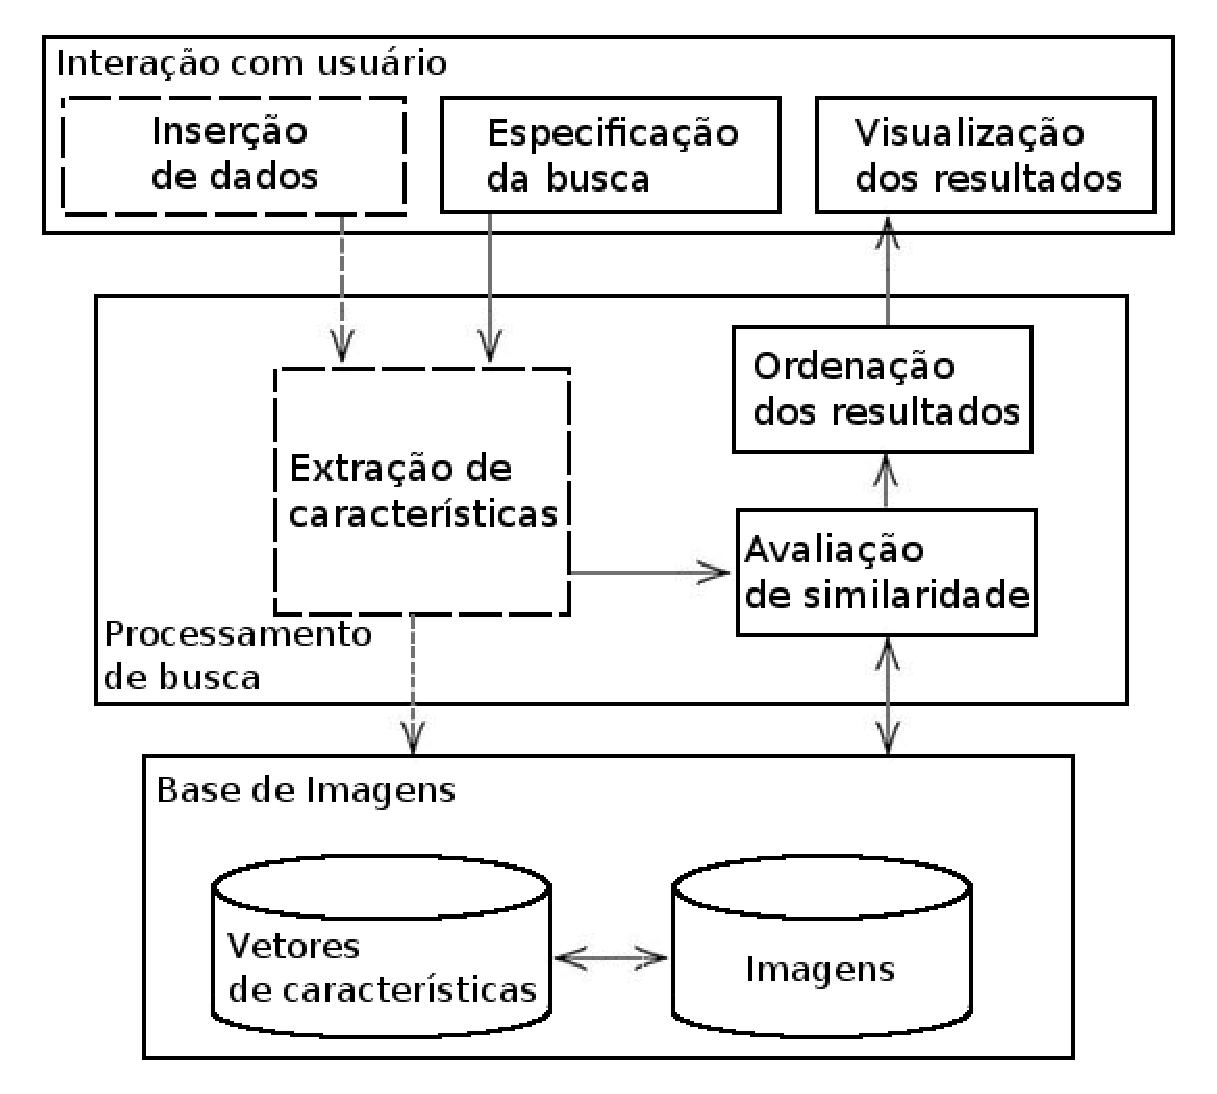
\includegraphics[width=0.65\textwidth]{cbir.eps}
\legend{Fonte: \citeonline{Torres:2006}.}
\end{figure}
 
Neste trabalho enfatizamos os processos de extração de características e de avaliação de similaridade em \emph{CBIR}, sendo esses processos destacados nas sub-seções a seguir.

\subsection{Extração de características}

O processo de extração de características das imagens forma o alicerce dos sistemas \emph{CBIR}. Tal processo se dá através de operações de processamento de imagens, cujo objetivo é extrair informação que seja semanticamente relevante dos atributos da imagem para a realização das buscas por similaridade de conteúdo. 

Os atributos comumente empregados para extração de características em \emph{CBIR} são a cor, a textura, a forma e a localização espacial dos elementos constituintes de uma imagem. 

A cor é o atributo mais empregado em \emph{CBIR}, pois a mesma permite discriminar uma ampla gama de imagens. Quando se utiliza esse atributo deve se considerar que o registro da cor em uma imagem varia consideravelmente com a orientação da superfície imageada, o posicionamento da câmera, a posição da fonte de iluminação e a maneira como a luz interage com os objetos imageados \cite{Smeulders:2000}. Ademais, a percepção humana da cor é um assunto complexo que ainda não está completamente elucidado \cite{Smeulders:2000}. De acordo com \citeonline{Torres:2006}, as técnicas de descrição por cores podem ser agrupadas em duas grandes classes dependendo se a informação de cor é codificada correlacionada com a sua distribuição espacial ou não. 

\begin{comment}Esses mesmos autores exemplificam como técnicas que não levam em consideração a distribuição espacial das cores os histogramas e os momentos de cores. 
\end{comment}

Atributos de textura são úteis na recuperação de imagens de satélites, bem como na busca de documentos digitalizados \cite{Smeulders:2000}. Essa é definida em termos de estruturas formadas por grupos de pixels que aparecem na imagem com certa periodicidade ou aleatoriedade. O método já consagrado para descrição de características de texturas é a matriz de co-ocorrência proposta por \citeonline{4309314}. No entanto, métodos baseados em transformações wavelet têm sido utilizados \cite{5376587}, mais notoriamente a transformada wavelet de Gabor \cite{531803}. Outra técnica que tem sido explorada na atualidade para descrição de texturas é a dimensão fractal multiescala \cite{Florindo:2013}. 

Informação relativa à localização espacial dos elementos de uma imagem permite, por exemplo, recuperar imagens de cenas fotográficas de paisagens externas, aonde distingue-se a localização do céu na região superior da imagem. Ademais, imagens fotográficas também tendem a apresentar em seu centro alguma informação significativa que difere do entorno da imagem, sendo essa informação útil no processo de recuperação de imagens de fotografias de pessoas, animais, etc.

A forma é uma característica intrínseca das imagens que é amplamente explorada pelo sistema de visão dos primatas para o reconhecimento de objetos. Progressos significativos têm sido alcançados no desenvolvimentos de sistemas de recuperação de imagens pelo conteúdo baseados nesse atributo.

Dentre as abordagens empregadas na obtenção de representações a partir das formas, a mais popular é a que as representa através de vetores de características. Tal representação permite que a similaridade entre as formas seja avaliada através de medidas de distância entre vetores, de baixo custo computacional. No entanto, a representação por vetores de características é pouco discriminativa, o que limita a sua acurácia em aplicações \emph{CBIR}.

Já na representação estrutural, as formas são divididas em um conjunto de partes constituintes, sendo cada parte representada individualmente através de vetores de características. O descritor é composto a partir desses vetores e da relação existente entre as partes, representadas através de estruturas de dados como grafos, árvores ou cadeias de caracteres. Uma vez que esses métodos comparam as formas a partir das suas estruturas, esses conseguem uma boa acurácia, porém a um custo computacional elevado.

Métodos de representação por transformação empregam transformadas como Wavelet, Fourier e Espaço-Escala para descrever as formas. Em \emph{CBIR}, o custo computacional das buscas deve levar em consideração o custo de se aplicar a transformada à forma de consulta. 

Por último, os métodos por correspondência, ou alinhamento, representam as formas diretamente no domínio espacial. Esses métodos determinam o grau de similaridade entre duas formas tentando alinhá-las e medindo a diferença residual existente entre as mesmas.

\citeonline{Belongie:2002} propuseram um descritor do contorno da forma denominado de \emph{shape context} que avalia a similaridade entre formas por correspondência de pontos. Esse descritor caracteriza a distribuição dos demais pontos do contorno em relação a um ponto de referência para cada ponto do contorno tomado como referência. 


\begin{comment}
As abordagens empregadas na obtenção de representações a partir das formas podem ser classificadas em 3 grandes categorias:

\begin{alineas}

\item representação por vetor de características: É a técnica mais popular de representação. Neste método, a forma é representada através de um vetor numérico e a similaridade entre as formas é avaliada através de uma distância entre vetores. 

\item representação por transformação: deformações são realizadas em uma forma a fim de transformá-la em outra. A similaridade entre as formas é medida pelo esforço necessário para se realizar a transformação.  

\item representação relacional: Nesta abordagem as formas são divididas em um conjunto de partes constituintes. Cada parte é individualmente representada através de vetores de características. O descritor é composto a partir destes vetores e da relação existente entre as partes.
\end{alineas}

Técnicas de representação por vetores de características são classificadas em duas grandes classes: técnicas baseadas em região e técnicas baseadas em contorno.
\end{comment}

\subsection{Medidas de similaridade}
O processo de recuperação de imagens pelo conteúdo requer que alguma medida seja empregada na avaliação da similaridade entre as representações das imagens. Nas técnicas de extração de características que resultam em representações vetoriais, as medidas de distância entre vetores são comumente empregadas para este fim. Desta forma, o grau de similaridade entre duas representações guarda uma relação inversa com a medida de distância correspondente. 

Uma medida de distância entre dois vetores $p$ e $q$ é considerada uma métrica de distância quando satisfaz as seguintes propriedades: 

\begin{alineas}
\item Positividade: $d(p,q) \geq 0$;  
\item Unicidade: $d(p,q) = 0 \Rightarrow p = q$;
\item Simetria: $d(p,q) = d(q,p)$;
\item Desigualdade triangular: $d(p,r) + d(r,q) \geq d(p,q)$.
\end{alineas}

Para as representações vetoriais dentro de um mesmo espaço dimensional, distâncias simples entre vetores, de baixo custo computacional, como as apresentadas na Tabela \ref{tbl:distance}, são empregadas. Já nos casos aonde a representação das imagens resulta em descrições de dimensões distintas, técnicas mais elaboradas, que utilizam programação dinâmica, são necessárias. Dentre essas técnicas a \emph{DSW} (\emph{Dynamic space warping}) tem sido empregada na avaliação de similaridade entre formas a partir de assinaturas extraídas dos seus contornos \cite{Alajlan20117}. 

\begin{table}
\centering
\caption{\label{tbl:distance}Medidas de distância entre vetores}
\begin{tabular}[]{ll}
\hline
Medida de distância&Fórmula matemática\\
\hline
Distância de Minkowski&$d(x,y) = \Big[\sum\limits_{i=1}^{n}(x_i-y_i)^m\Big]^\frac{1}{m}$\\
Distância euclidiana&$d(x,y) = \Big[\sum\limits_{i=1}^{n}(x_i-y_i)^2\Big]^\frac{1}{2}$\\
Distância city-block&$d(x,y)= \sum\limits_{i=1}^{n}|x_i-y_i|$\\
Distância Chebyshev&$d(x,y)= \max\limits_{i}|x_i-y_i|$\\
Separação angular&$d(x,y)=\frac{\sum\limits_{i=1}^n{x_iy_i}}{\Big[\sum\limits_{i=1}^n{x_i^2}\sum\limits_{i=1}^n{y_i^2}\Big]^\frac{1}{2}}$\\
Canberra&$d(x,y) = \sum\limits_{i=1}^n\frac{|x_i-y_i|}{x_i+y_i}$\\
\hline
\end{tabular}
\end{table}

\section{\label{chap:contour}Descritores do contorno das formas}

Os estímulos visuais, ao qual os sistemas de visão biológicos estão submetidos, apresentam um elevado grau de redundância de informação. No processamento dessa informação, tais sistemas buscam eliminar essas redundâncias, retendo apenas a quantidade de informação necessária para o desempenho da tarefa requerida.  

Em visão computacional e reconhecimento de padrões, dá-se o nome a esse processo de eliminação das redundâncias de extração de características. Esta etapa de baixo nível busca encontrar informação relevante em uma imagem e representá-la convenientemente para a realização de uma tarefa específica de visão computacional. Uma vez que o processo de extração de características determina o desempenho de um sistema de visão computacional, este recebe especial atenção no desenvolvimento de tais sistemas.

Dentre os atributos dos quais se realizam a extração de características, a forma é considerada a mais relevante em diversas aplicações de visão artificial pela riqueza de informações que esta possui. Uma forma é obtida quando um objeto de interesse é identificado e segmentado em uma imagem. 
 De acordo com \citeonline{Zhang:2004}, para que se obtenha uma representação conveniente com base nesse atributo, deve-se buscar por informações que tenham importância em sua percepção, seja no contorno ou na região que a delimita. 

Obter uma representação, ou descrição, de objetos a partir de formas planas é uma tarefa complexa. Isso porque quando projetamos os objetos tridimensionais do mundo real em duas dimensões, perdemos as informações de uma das dimensões. Como resultado temos uma representação bidimensional parcial do objeto projetado. O problema torna-se ainda mais complexo se levarmos em conta que a forma é frequentemente corrompida por ruídos, defeitos, distorções arbitrárias e oclusões.

\citeonline{Zhang:2004} classificam as técnicas de representação de formas em duas grandes classes de métodos: os baseados em contorno e os baseados em região. Nos métodos baseados em região as características são extraídas de toda região da forma, enquanto que nos métodos baseados em contorno, as características são extraídas apenas da borda. Os referidos autores ainda subdividem cada classe de métodos em métodos estruturais e globais. Essa subdivisão é baseada em se a forma como um todo é utilizada na representação ou se a representação é obtida de partes, segmentos e seções das formas. 

A Figura \ref{fig:folha_contorno1} ilustra as etapas envolvidas no processo de representação de uma forma. Temos nesse caso a segmentação da imagem por limiar seguida da extração do contorno. Com base no contorno, obtém-se uma variedade de representações, na forma de sinais, adequadas para as tarefas de comparação, classificação e reconhecimento de formas.

Neste trabalho  enfatizamos a aplicação de técnicas de processamento de sinais para a obtenção de representações globais do contorno das formas, uma vez que tais técnicas têm sido empregadas com sucesso para esse propósito \cite{Costa:2009}. 

\begin{comment}
Técnicas baseadas em contorno de formas exploram apenas a região da borda da forma. Há dois tipos de abordagens para extração de características do contorno das formas: global e estrutural. Na abordagem global a forma não é dividida em sub-partes e um vetor de características que representa toda a borda é obtido para representar a forma. Na abordagem estrutural a borda da forma é particionada em segmentos, denominados de primitivas mediante algum critério. A representação final é geralmente uma cadeia de caracteres, um grafo ou uma árvore.
\end{comment}



%representar uma forma consiste em caracterizá-la através de um conjunto de características que permitam reconstruir-la exatamente ou com um certo grau de precisão. Os mesmos autores classificam os métodos de representação das formas em três grandes grupos: por contorno, por região e por transformação.
    

\begin{figure} 
\caption{\label{fig:folha_contorno1} Obtenção da forma e do contorno da imagem de uma folha.}
%\includegraphics[width=\textwidth,clip,trim=12mm 188mm 27mm 75mm]{figura_folha.png}
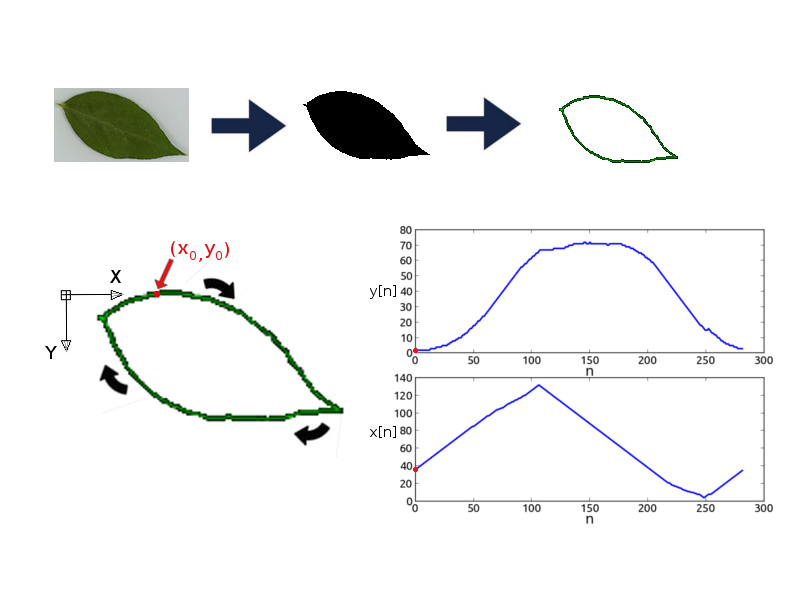
\includegraphics[width=\textwidth,clip,trim=10mm 145mm 36mm 26mm]{figura_folha_v3.png}
%\legend{Fonte: próprio autor}
\end{figure}

\subsection{\label{sec:Assinatura}Representações por assinaturas
}

\citeonline{Costa:2009} definem assinatura de uma forma como sendo um sinal discreto uni-dimensional que descreve algumas das características do seu contorno ou da sua região. Devido a redução de dimensionalidade, as assinaturas do contorno são representações compactas das formas. 

Estas podem ser utilizadas diretamente como descritores, porém o custo computacional envolvido em sua comparação direta é elevado. Isso porque as assinaturas frequentemente não são totalmente insensíveis a rotação, translação e escalamento das formas, bem como variam no total de amostras conforme varia a resolução das imagens. 

Algumas assinaturas são mais sensíveis a ruído e a pequenas distorções dos contornos, tornando necessário realizar filtragens. Embora melhore a robustez, tal processo acarreta em alguma perda de informação.

Várias assinaturas vêm sendo empregadas na literatura para descrição de formas nas mais diversas aplicações, tais como a distância ao centróide, as coordenadas complexas, ângulo tangente, ângulo acumulativo, curvatura, área e comprimento da corda \cite{Zhang:2004}.

\subsubsection*{\label{sec:Rep_par}Coordenadas paramétricas}
A representação por coordenadas paramétricas consiste nas coordenadas dos pontos amostrados do contorno, representados a partir de um sistema de coordenadas pré-estabelecido, percorrendo-o sequencialmente em sentido horário ou anti-horário. Para o contorno discreto $\mathbf{C}$, com $N$ amostras, representado num sistema de coordenadas cartesianas, tal processo origina um conjunto de tuplas $\mathbf{C}[n] = \big(\mathbf{x}[n]\:\text{,}\:\mathbf{y}[n]\big)$, $n \in {\{0\:\text{,}\:1\:\text{,}\:\dotsc\:\text{,}\:N-1\}}$, cujas componentes $\mathbf{x}[n]$ e $\mathbf{y}[n]$ são sinais discretos vetoriais das coordenadas amostradas do contorno.

Na Figura \ref{fig:folha_contorno} estão representados os sinais obtidos para o contorno da folha da Figura \ref{fig:folha_contorno1} com a amostragem $N = 280$ pontos. Em vermelho está destacado o ponto de origem aonde a varredura, em sentido horário, se inicia. Os dois pontos observados aonde a evolução do sinal $\mathbf{x}[n]$ inverte sua tendência (de crescente para decrescente e de decrescente para crescente) correspondem aos pontos mais salientes da folha. Já o platô observado no sinal $\mathbf{y}[n]$ corresponde a região da parte inferior da folha, em que quase não se observa variações do contorno ao longo do eixo $Y$.
   
\begin{figure} 
\caption{\label{fig:folha_contorno} Processo de obtenção da representação paramétrica do contorno da folha da figura \ref{fig:folha_contorno1}.}
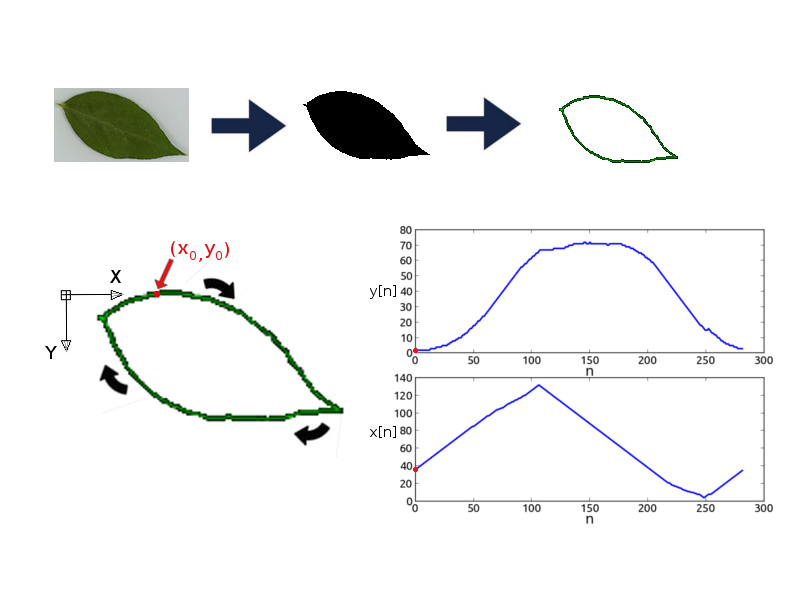
\includegraphics[width=\textwidth,clip,trim= 12mm 30mm 10mm 77mm]{figura_folha_v3.png}
%\legend{Fonte: próprio autor}
\end{figure}

Outra representação paramétrica para o contorno é obtida compondo-se um sinal complexo $\mathbf{z}[n] = \mathbf{x}[n] + j\mathbf{y}[n]$, $j = \sqrt{-1}$, $n \in {\{0\:\text{,}\:1\:\text{,}\:\dotsc\:\text{,}\:N-1\}}$. Essa representação é conveniente quando se deseja realizar extração de características do contorno através de operações de processamento de sinais. A figura \ref{fig:folha_complex} ilustra o módulo e a fase da representação complexa do contorno da folha da figura \ref{fig:folha_contorno1}. 

\begin{figure} 
\caption{\label{fig:folha_complex} Representação paramétrica do contorno da folha da Figura \ref{fig:folha_contorno1} como sinal complexo.}
\centering
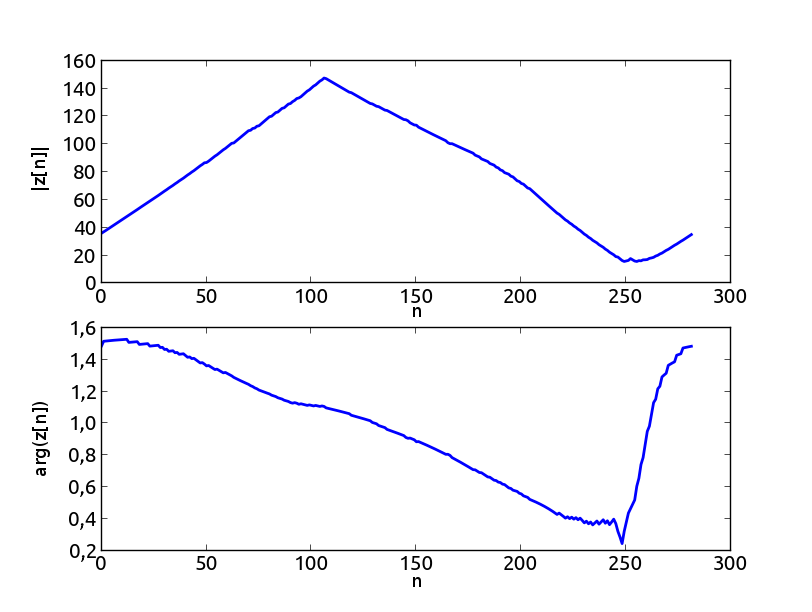
\includegraphics[width=0.75\textwidth]{folha_complex_v3.png}
%\legend{Fonte: próprio autor}
\end{figure} 

Embora sejam descritivas, as representações por coordenadas paramétricas apresentam o inconveniente de não serem invariantes a translação, rotação ou escalamento das formas. Por isso são consideradas \color{red} representações intermediárias (????) \color{black}, pois outras assinaturas, com propriedades de invariância, podem ser obtidas partindo-se de tais representações \cite{Kindratenko:2003}.

\subsubsection*{Curvatura\label{sec:curvatura}}

A curvatura é uma assinatura do contorno da forma com importantes propriedades geométricas, o que motiva sua utilização para obtenção de descritores. Há evidências biológicas de que as propriedades desta assinatura sejam exploradas pelo sistema de visão dos primatas nas tarefas de reconhecimento de formas \cite{Costa:2009}. Na Tabela \ref{tbl:curv} estão destacadas as principais propriedades que a curvatura apresenta.  

\begin{table}
\centering
\caption{\label{tbl:curv} Propriedades da curvatura e as características geométricas que essas representam.}
\begin{tabular}[]{ll}
\toprule
\multicolumn{1}{c|}{Propriedade} & \multicolumn{1}{c}{Característica da forma}\\ 
\hline
Máximo valor absoluto & Ponto saliente \\
Máximo valor positivo & Saliência convexa \\
Mínimo valor negativo & Saliência côncava \\
Valores constantes e nulos & Segmentos retilíneos \\
Valores constantes e não nulos & Segmentos circulares \\
Cruzamentos de zero & Pontos de inflexão \\ \bottomrule
\end{tabular}
\legend{Fonte: \citeonline{Costa:2009}}
\end{table}

A função curvatura ($K(l)$), para uma curva contínua fechada $C = \big(x(l)\:\text{,}\:y(l)\big)$,  cujo perímetro é $L$ e que encontra-se parametrizada em $l \in [0\text{,}L]$, é definida como sendo \cite{Kindratenko:2003}:

\begin{equation} \label{eq:curvatura}
K(l) = \frac{x^{'}(l)y^{''}(l)-x^{''}(l)y^{'}(l)}{((x^{''}(l))^{2}+(y^{''}(l))^{2})^{\frac{3}{2}}}\text{,}
\end{equation}

\noindent 
sendo $\big(x^{'}(l) \text{, }y^{'}(l)\big)$ e $\big(x^{''}(l)\text{ , }y^{''}(l)\big)$ as derivadas primeira e segunda das coordenadas paramétricas da curva, respectivamente.

Sob o aspecto computacional, o cálculo da curvatura do contorno de uma forma requer que o mesmo seja espacialmente amostrado e discretizado. Tal processo torna o cálculo das derivadas da Equação \ref{eq:curvatura} sensível ao ruído e inviável, o que limita a aplicação direta da curvatura para a obtenção de descritores. 

A Figura \ref{fig:cir1} ilustra tal efeito para uma imagem de forma circular. A Figura \ref{fig:cir1}a representa o gráfico da curvatura teórica, obtida analiticamente, pela aplicação da Equação \ref{eq:curvatura} ao contorno parametrizado do círculo de mesmo raio ao do círculo da Figura \ref{fig:cir1}b. Já na  Figura \ref{fig:cir1}c, temos a curvatura obtida computacionalmente a partir do contorno discreto extraído do círculo da Figura \ref{fig:cir1}b. Nota-se que a curvatura da Figura \ref{fig:cir1}a (analítica) tem um valor constante $K(l) = \frac{1}{r}$, sendo $r$ o raio do círculo central, enquanto que a curvatura Figura \ref{fig:cir1}c (computacional) varia significativamente em torno do valor analítico esperado, como mostra a Figura \ref{fig:cir1}. 

\begin{figure}[h!]
  \caption{\label{fig:cir1} Efeito do ruído na estimativa computacional da curvatura para uma forma circular.}
  \centering
  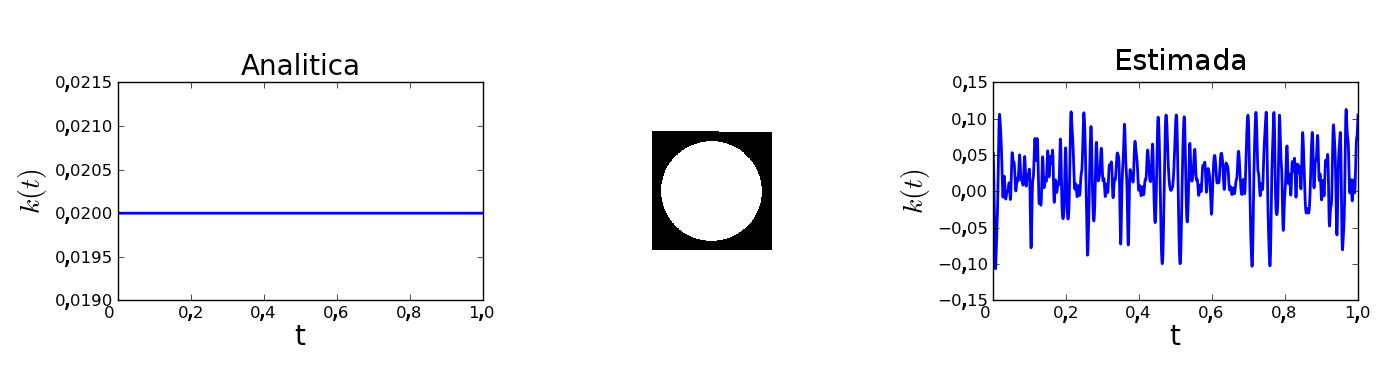
\includegraphics[width=\textwidth, clip, trim=20mm 5mm 0mm 0mm]{curv_cir.png}
  %\legend{Fonte: próprio autor}
\end{figure}

Diversas estratégias foram propostas na literatura para contornar o problema da sensibilidade ao ruído do cálculo computacional da curvatura. Trabalhos clássicos, como os de \citeonline{5009188} e \citeonline{LynnBeus1987291} estimam a curvatura a partir do ângulo formado entre vetores obtidos a partir dos pontos do contorno. \citeonline{Cazals:2003} e \citeonline{Shi20022051} apresentaram trabalhos que utilizavam métodos para estimação da curvatura por interpolação de pontos. 

\citeonline{149591} introduziram um método que suaviza o contorno, através da convolução do mesmo com um filtro passa-baixas \color{red}gaussiano\color{black}, antes de se calcular a curvatura.

\begin{figure}[h!]
 \caption{\label{fig:curv_folha} Curvatura estimada do contorno da folha da Figura \ref{fig:folha_contorno1} através de método computacional.}
  \centering
  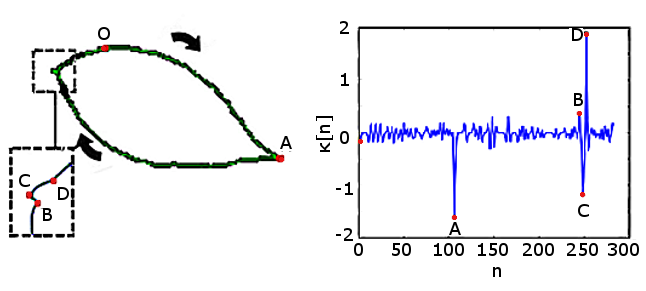
\includegraphics[width=0.75\textwidth]{curv_folha_v2.png}
%\legend{Fonte: próprio autor}
\end{figure}

A Figura \ref{fig:curv_folha} mostra a curvatura estimada, para o contorno da folha da Figura \ref{fig:folha_contorno1}, através do método proposto por \citeonline{149591}. O contorno foi previamente suavizado com um filtro gaussiano com desvio padrão $\sigma = 20$. Os pontos aonde a curvatura apresenta os picos em destaque correspondem aos pontos salientes da folha. 

\begin{comment}
Particularmente, métodos de extração de características multiescala do contorno a partir da curvatura conseguem superar o problema supracitado aplicando filtragens passa-baixa a representação paramétrica do contorno antes de se calcular a curvatura. 
\end{comment}

\subsubsection*{Distância ao centróide}
Uma assinatura simples pode ser obtida calculando-se a distância de cada coordenada do contorno ao centróide da forma. Esse último consiste, para um contorno discreto de $N$ amostras, em um vetor calculado, a partir das coordenadas do contorno, pela seguinte equação: 

\begin{equation}
\big(x_{c}\:\text{,}\:y_{c}\big) = \Big(\frac{1}{N}\sum^{N}_{i=0}{\mathbf{x}[i]}\:\text{,}\:\frac{1}{N}\sum^{N}_{i=0}{\mathbf{y}[i]}\Big)\text{.}
\end{equation}

O sinal da distância ao centróide $\mathbf{dc}[n]$ é dado por:

\begin{equation}
\mathbf{dc}[n] = \sqrt{(\mathbf{x}[n] - x_c)^2 + (\mathbf{y}[n] - y_c)^2}\text{.}
\end{equation}

Essa assinatura tem a propriedade de ser invariante a translação da forma, o que a torna independente do sistema de coordenadas adotado na parametrização do contorno. Embora não seja invariante a escala e a rotação, tais invariâncias podem ser obtidas, como sugerem alguns trabalhos. 

Empregando um processo de sub-amostragem e de normalização pelo maior valor, \citeonline{Wang:2000} tornam essa assinatura invariante a escala. Para se alcançar invariância a rotação os referidos autores sugerem que, no processo de avaliação de similaridade entre duas assinaturas, seja realizado o deslocamento cíclico de uma das assinaturas até que se obtenha a maior similaridade.

Já \citeonline{Zhang:02} utilizam a distância ao centróide como assinatura para se obter os descritores de Fourier. Tal estratégia garante as propriedades de invariância a rotação e a escala.

\begin{figure}[h!]
  \caption{\label{fig:cd} Assinatura da distância ao centróide para o contorno da folha da Figura \ref{fig:folha_contorno1}}
  \centering
  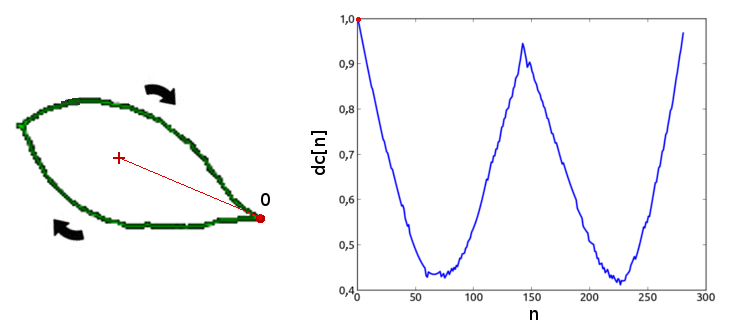
\includegraphics[width=0.75\textwidth]{cd_v2.png}
  %\legend{Fonte: próprio autor}
\end{figure}

A Figura \ref{fig:cd} ilustra a assinatura da distância ao centróide para a folha da Figura \ref{fig:folha_contorno1}. Neste exemplo, a assinatura foi normalizada a partir da distância máxima ao centróide, que corresponde ao ponto vermelho demarcado tanto no gráfico como no contorno. 

\subsubsection*{Sequência de ângulos}

A assinatura de sequência de ângulos é obtida a partir do ângulo formado entre vetores construídos a partir das coordenadas do contorno parametrizado conforme ilustrado na Figura \ref{fig:angulo}. 

Para um dado ponto pertencente ao contorno, de coordenadas $(x_i\:\text{,}\:y_i)$, obtemos os vetores $\overrightarrow{v_1}$ e $\overrightarrow{v_2}$. O primeiro vetor é formado pela diferença entre as coordenadas $(x_i\:\text{,}\:y_i)$ e $(x_{i-p}\:\text{,}\:y_{i-p})$, enquanto o segundo vetor é formado pela diferença entre as coordenadas $(x_{i+p}\:\text{,}\:y_{i+p})$ e $(x_i\:\text{,}\:y_i)$. 

Da propriedade do produto interno, temos a seguinte relação dessas coordenadas com o ângulo $\theta_i$, formado entre os vetores $\overrightarrow{v_1}$ e $\overrightarrow{v_2}$:

\begin{equation}
\overrightarrow{v_1}. \overrightarrow{v_2} = |\overrightarrow{v_1}||\overrightarrow{v_2}|\cos{\theta_i}=(x_i-x_{i-p})(x_{i+p}-x_i)+(y_i-y_{i-p})(y_{i+p}-y_i)\text{.}
\end{equation}

Logo, o ângulo $\theta_i$ é calculado através da seguinte expressão:

\begin{equation}
\theta_i = \arccos{\Big[\frac{(x_i-x_{i-p})(x_{i+p}-x_i)+(y_i-y_{i-p})(y_{i+p}-y_i)}{\sqrt{\big[(x_i-x_{i-p})^2+(y_i-y_{i-p})^2\big]\big[(x_{i+p}-x_i)^2+(y_{i+p}-y_i)^2\big]}}\Big]}\text{.}
\end{equation}

O parâmetro $p$ controla a sensibilidade da assinatura a características locais do contorno. Valores grandes desse parâmetro resultam em uma assinatura menos sensível a características locais, enquanto que valores pequenos fazem com que a assinatura seja mais sensível a características locais.  Em \cite{Fotopoulou:2013} essa assinatura foi empregada para identificação de espécies vegetais a partir do contorno das folhas.

\begin{figure}[h!]
  \caption{\label{fig:angulo} Ilustração geométrica do método de obtenção da assinatura de sequência de ângulos.}
  \centering
  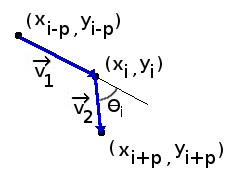
\includegraphics[width=0.2\textwidth]{angulo.png}
  %\legend{Fonte: próprio autor}
\end{figure}

\subsubsection*{Invariantes integrais}

Uma vez que as assinaturas obtidas através de operadores diferenciais são sensíveis a ruídos e a pequenas deformações do contorno, \citeonline{Manay:2006} propuseram os invariantes integrais como uma representação inerentemente robusta a estes artefatos.

Seja $C \subset \mathbb{R}^2$ um contorno fechado e $\overline{C}$ sua área interior.
A função 

\begin{equation}
 B_r(p,x) = \left\{
  \begin{array}{l l}
    1 & \quad |p-x|\leq r\\
    0 & \quad |p-x|> r
  \end{array} \right.
\end{equation} 

\noindent
indica se um ponto $x$ pertence ou não ao interior de um disco $B_r$,  centrado em $p$ e de raio $r$.

Empregando a função acima especificada, obtém-se uma assinatura invariante integral através da seguinte equação: 

\begin{equation}
A(p) = \int_{\overline{C}}{B_r(p,x)dx}\text{,}
\end{equation} 

\noindent
sendo $p \in [0,L]$ e $L$ o perímetro do contorno.

A Figura \ref{fig:Aii} ilustra, do ponto de vista geométrico, o processo de obtenção da assinatura invariante integral. O disco $B_r(p)$ é centrado em cada ponto $p(s)$ pertencente ao contorno e a área de interseção entre $B_r(p)$ e a região interna ao contorno $\overline{C}(s)$ é determinada.

\begin{figure}[h!]
  \caption{\label{fig:Aii} Ilustração geométrica do método de obtenção da assinatura invariante integral.}
  \centering
  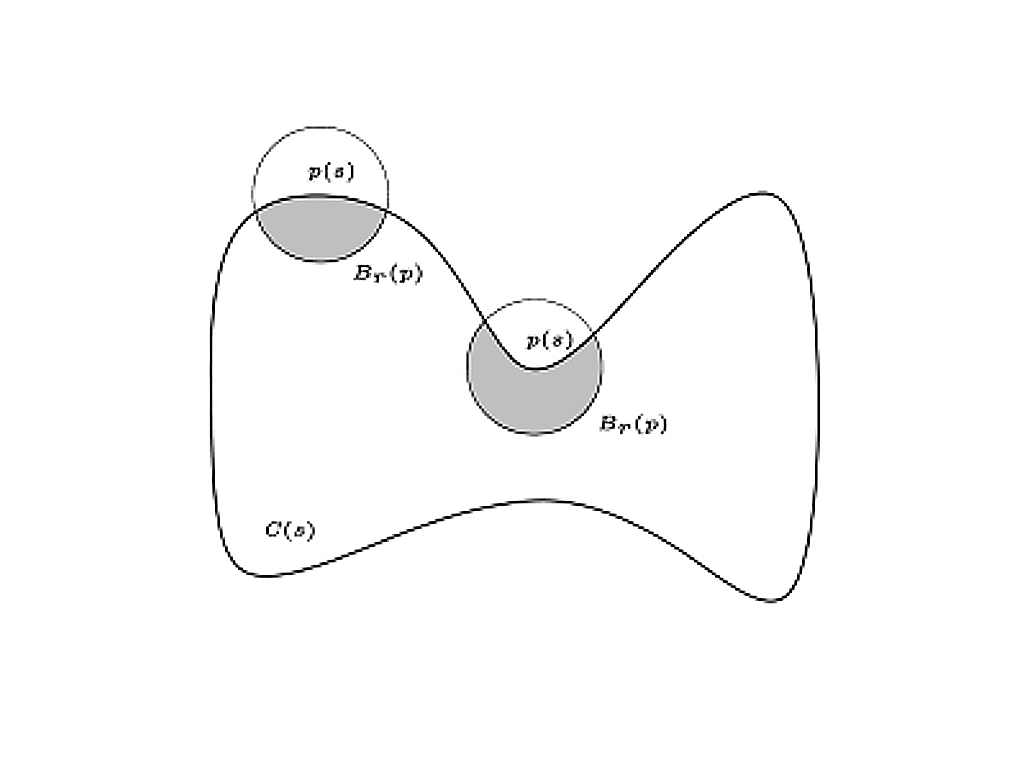
\includegraphics[width=0.75\textwidth, clip, trim = 0mm 55mm 0mm 40mm]{aii.png}
  \legend{Fonte: \citeonline{Manay:2006}.}
\end{figure}

\subsection{Representações multiescala\label{chap:multiescala}} 

Qualquer método que se proponha a descrever características das formas com base em contornos deve ser capaz de representá-las de forma confiável e precisa. 

\begin{comment}Segundo \citeonline{149591}, esses devem satisfazer os seguintes requisitos:

\begin{alineas}
\item Invariância: duas curvas que tenham a mesma forma devem ter a mesma representação;
\item Unicidade: duas curvas que não tenham a mesma forma devem apresentar diferentes representações;
\item Estabilidade: pequenas variações observadas entre duas curvas devem resultar em pequenas variações em suas representações;
\item Eficiência: uma vez que alguns sistemas de visão computacional apresentam requisitos de tempo real, a descrição deve ser computacionalmente eficaz, demandando poucos recursos de memória e de processamento;
\item Fácil implementação: é recomendável que os métodos de descrição sejam simples e de fácil implementação de modo a requerer menos tempo de implementação e depuração; 
\item Relação com propriedades específicas das formas: o método de descrição deve ser capaz de representar propriedades das formas que este descreve.
\end{alineas}

Os referidos autores afirmam que muitos dos métodos de extração encontrados em visão computacional falharam em satisfazer um ou mais dentre estes requisitos.
\end{comment}

Embora carregue grande parte da informação a respeito das formas, o contorno é  sensível a ruídos, oclusões e variações das formas.  Em outros casos, o contorno não se apresenta completamente disponível, com regiões disjuntas e descontinuidades. Tais aspectos comprometem a confiabilidade e a precisão das assinaturas baseadas em contorno.  

A descrição multiescala do contorno das formas vêm se mostrando uma alternativa viável para superação de tais problemas. 

Esta técnica se baseia no método proposto por \citeonline{Witkin:1983} e \citeonline{Koenderink:1984} para análise de sinais em vários níveis de resolução. Esses autores introduziram o conceito de fator de escala, cujo ajuste determina o grau de resolução na qual ocorre a análise do sinal. 

\begin{figure}[h!]
  \caption{\label{fig:ms} Método de análise multiescala a partir da assinatura do contorno de uma forma.}
  \centering
  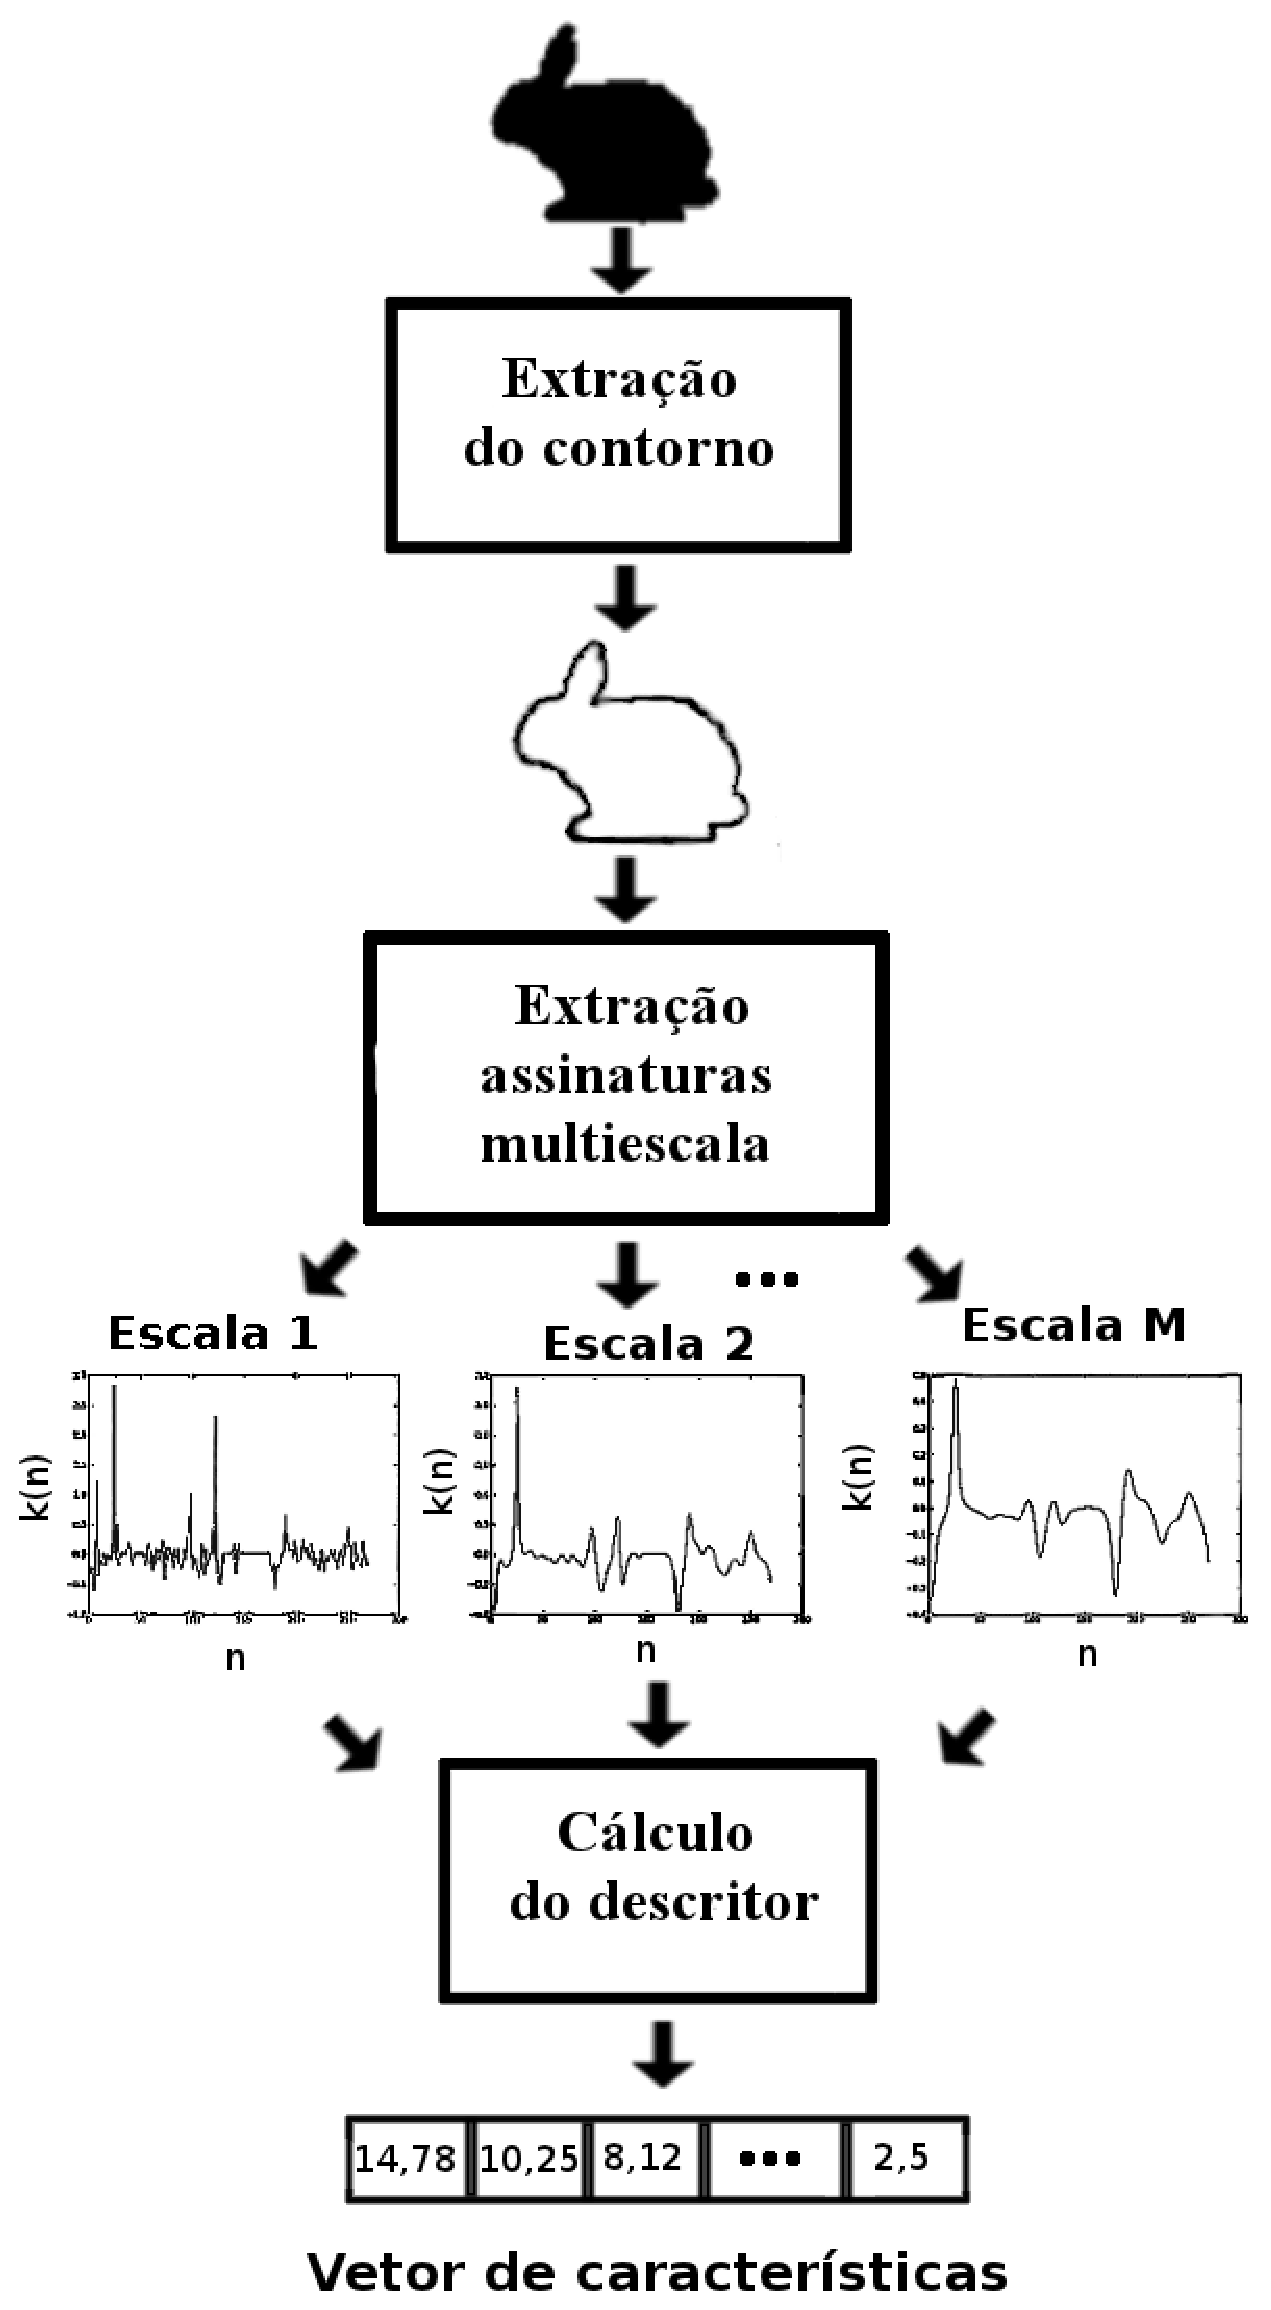
\includegraphics[width=0.45\textwidth]{feature_extraction.eps}
 % \legend{Fonte: próprio autor}
\end{figure}

A Figura \ref{fig:ms} ilustra o processo para obtenção de uma representação multiescala de um sinal unidimensional discreto $k[n]$ que represente o contorno de uma forma, tal como as assinaturas apresentadas na Seção \ref{sec:Assinatura}. Emprega-se nesse processo uma função de transformação $F[n,\sigma]$, geralmente com características de filtragem passa-baixas e com frequência de corte $\sigma$. Na função de transformação, a referida frequência de corte corresponde ao fator de escala na qual o sinal $k[n]$ será analisado. 

Para um vetor de escalas $\sigma = (\sigma_1\:\sigma_2\:\ldots\:\sigma_M) $, a representação multiescala consiste em um vetor de sinais $k[n,\sigma] = (k[n,\sigma_1]\:k[n,\sigma_2]\:\ldots\:k[n,\sigma_N])$, sendo cada termo $k[n,\sigma_i]$ obtido através de
\begin{equation}\label{eq:ms1}
k[n,\sigma_i] = F[n,\sigma_i]*k[n]\text{,}
\end{equation}

\noindent
 aonde o operador $*$ denota a convolução entre o sinal $k[n]$ e a transformação $F[n,\sigma_i]$.  Assim, cada elemento de $k[n,\sigma]$ corresponde ao sinal $k[n]$ analisado na escala $\sigma_i$.

No caso de curvas planas, a análise multiescala permite descrevê-las em vários níveis de detalhes e de abstração a partir de suas assinaturas, tornando a representação mais discriminativa que os métodos que empregam medidas quantitativas globais, como área, perímetro e compacidade, devido a sua robustez e estabilidade \cite{4756134}.    

\subsubsection*{Curvaturas Multiescala\label{subsec:curvMS}}

Inspirados na técnica de \citeonline{Witkin:1983} e \citeonline{Koenderink:1984}, \citeonline{149591} propuseram um método para análise multiescala do contorno através da assinatura da curvatura. O referido método emprega como função de transformação um filtro passa-baixas gaussiano, $g_{\sigma}(l) = \frac{1}{\sigma\sqrt{2\pi}}e^{\frac{l^2}{2\sigma^2}}$, que suaviza o contorno antes do cálculo de sua curvatura. Nesse caso, o ajuste do desvio padrão da função gaussiana ($\sigma^2$) atua como fator de escala, regulando a largura de banda do filtro e o nível de suavização do contorno.

%Desta forma, o sinal da curvatura é obtido em múltiplas escalas uma vez que a suavização do contorno possibilita o cálculo das derivadas. 


No caso contínuo temos as coordenadas do contorno suavizado realizando a convolução entre as coordenadas do contorno parametrizado $C(l) = (x(l)\text{,}y(l))$ e o filtro gaussiano:  

\begin{equation}
x_{\sigma}(l) = x(l) * g_{\sigma}(l) = \int^{\infty}_{-\infty}{x(v)g_{\sigma}(l-v)}dv \text{ e}
\end{equation}
\begin{equation}
y_{\sigma}(l) = y(l) * g_{\sigma}(l)=\int^{\infty}_{-\infty}{y(v)g_{\sigma}(l-v)}dv
\end{equation}\text{.}

Para o cálculo das derivadas $x^{'}_{\sigma}(l)\text{, }y^{'}_{\sigma}(l)\text{, }x^{''}_{\sigma}(l) \text{ e }y^{''}_{\sigma}(l)$, necessárias para o cálculo da curvatura do contorno suavizado, temos, pelas propriedades da convolução, $x^{'}_{\sigma}(l) = x(l) * g^{'}_{\sigma}(l)\text{, }y^{'}_{\sigma}(l) = y(l) * g^{'}_{\sigma}(l)\text{, }x^{''}_{\sigma}(l) = x(l) * g^{''}_{\sigma}(l)\text{ e }
y^{''}_{\sigma}(l) = y(l) * g^{''}_{\sigma}(l)$.

O cálculo da curvatura do contorno suavizado $K_{\sigma}(l)$ se dá através da equação \ref{eq:curvatura}, substituindo-se $x^{'}(l)\text{, }\:y^{'}(l)\text{, }\:x^{''}(l)\:\text{ e }\:y^{''}(l)$ por $x^{'}_{\sigma}(l)\text{, }\:y^{'}_{\sigma}(l)\text{, }\:x^{''}_{\sigma}(l)\:\text{ e }\:y^{''}_{\sigma}(l)$, respectivamente, ou seja,

\begin{equation} \label{eq:curvatura_ms}
K_{\sigma}(l) = \frac{x_{\sigma}^{'}(l)y_{\sigma}^{''}(l)-x_{\sigma}^{''}(l)y_{\sigma}^{'}(l)}{((x_{\sigma}^{''}(l))^{2}+(y_{\sigma}^{''}(l))^{2})^{\frac{3}{2}}}\text{.}
\end{equation}

Uma outra abordagem utilizada para se calcular a curvatura multiescala, que foi proposta por \citeonline{Cesar:1996} e adotada nesta tese, opera com a representação do contorno no domínio da frequência. A partir da transformada de Fourier das coordenadas do contorno suavizado $X_{\sigma}(f) = F\big\{x_{\sigma}(l)\big\}$ e $Y_{\sigma}(f) = F\big\{y_{\sigma}(l)\big\}$. Os referidos autores calculam derivadas utilizando a propriedade da derivada da transformada de Fourier, ou seja:

\begin{equation}
x_{\sigma}^{'}(l) = F^{-1}\big\{2 \pi j f  X_{\sigma}(f)\big\}
\end{equation}

\begin{equation}
y_{\sigma}^{'}(l) = F^{-1}\big\{2 \pi j f  Y_{\sigma}(f)\big\}
\end{equation}

\begin{equation}
x_{\sigma}^{''}(l) = F^{-1}\big\{- (2 \pi f)^2 X_{\sigma}(f)\big\}
\end{equation}

\begin{equation}
y_{\sigma}^{''}(l) = F^{-1}\big\{- (2 \pi f)^2 Y_{\sigma}(f)\big\}
\end{equation}, aonde $F^{-1}\big\{X(f)\big\}$ denota a transformada de Fourier inversa do sinal $X(f)$.

\begin{comment}
\begin{equation}
X(f) = F\big\{x(l)\big\} = \int\limits^\infty_\infty x(l)e^{-2 \pi j f l}dl
\end{equation}

\begin{equation}
x(l) = F^{-1}\big\{X(f)\big\} \int\limits^\infty_\infty X(f)e^{2 \pi j f l}df
\end{equation}
\end{comment}

Na suavização do contorno no domínio da frequência, ao invés da convolução, realiza-se o produto dos sinais $X(f)$ e $Y(f)$ com a transformada de Fourier da expressão do filtro gaussiano:

\begin{equation}
X_\sigma(f) = X(f).G_\sigma(f)
\end{equation}

\begin{equation}
Y_\sigma(f) = Y(f).G_\sigma(f)
\end{equation}, sendo

\begin{equation}
G_\sigma(f) = F\big\{ g_{\sigma}(l)\big\} = e^{-2 \pi^2 f^2 \sigma^2}\text{.}
\end{equation}

\begin{figure}[h!]
  \caption{\label{fig:curv_ms} Curvatura multiescala do contorno da folha da Figura \ref{fig:folha_contorno1}.}
  \centering
  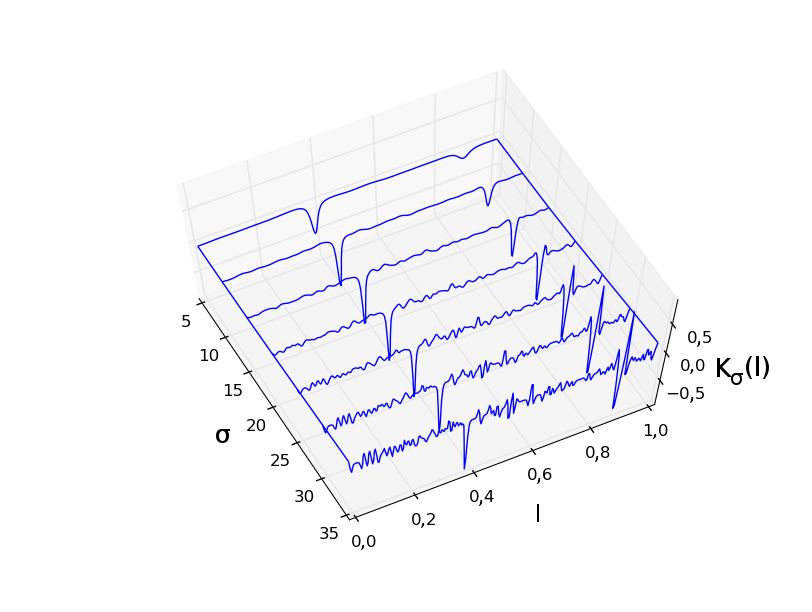
\includegraphics[width=0.75\textwidth]{curvograma_v2.png}
  \legend{Fonte: próprio autor}
\end{figure}

A Figura \ref{fig:curv_ms} ilustra a evolução do sinal de curvatura do contorno da folha da Figura \ref{fig:folha_contorno1} para diferentes níveis de suavização. Os picos da curvatura que se preservam nas escalas de baixa resolução correspondem às informações mais salientes do contorno, que o caracterizam globalmente. As informações de detalhes, que tendem a desaparecer nas escalas de baixa resolução e se preservam nas escalas de alta resolução, representam as características mais especificas do contorno.

\subsubsection*{Energia de dobramento multiescala\label{subsec:BE}}

\citeonline{Young:1974} propuseram a energia de dobramento como uma medida de complexidade para análise de formas biológicas. Conceitualmente, esta é definida como sendo a energia necessária para se modificar uma forma, através de deformações, ao seu estado de menor energia, ou seja, um círculo do mesmo perímetro da forma deformada.

A maneira mais direta de se obter a energia de dobramento de um contorno fechado é a partir de sua curvatura pela seguinte expressão:

\begin{equation}\label{eq:be}
E = \frac{1}{L}\int\limits_{l}K^2(l)dl\text{,}
\end{equation}
\noindent
sendo $L$ o perímetro do contorno e a integral calculada ao longo do comprimento de seu arco. O resultado da equação \ref{eq:be} é um escalar que representa a energia média do sinal da curvatura.

\begin{comment}
A energia de dobramento multiescala é obtida a partir da curvatura multiescala repetindo-se o cálculo da equação \ref{eq:be} para diferentes níveis de suavização do contorno. Isso resulta em um vetor de características composto por escalares decorrentes da curvatura multiescala para cada uma das escalas empregadas na suavização do contorno e cálculo da curvatura. 
\end{comment}

A energia de dobramento multiescala foi introduzida por \citeonline{Costa:1997} para a análise de formas de neurônios. Nesta tese investigamos sua utilização como um descritor de propósito geral em recuperação de formas pelo conteúdo. Para um contorno discreto, com $N$ pontos, representado na forma complexa $z[n] = x[n]+jy[n] \text{,} \quad n \quad \epsilon \quad [0, \quad 1, \quad \ldots \quad , \quad N-1]$, a energia de dobramento é dada por: 

\begin{equation}
E_{be} = \frac{L^{2}}{N}\sum_{n=0}^{N-1}K^{2}[n]\text{,}
\label{eq:ebe}
\end{equation}
\noindent
sendo o perímetro do contorno elevado ao quadrado ($L^2$) uma constante de normalização para que o descritor tenha invariância a escala. A curvatura discreta $K[n]$ é calculada a partir de $z[n]$ através da seguinte expressão:

\begin{equation}
K[n] = \frac{-Im(z^{'}[n](z^{''}[n])^{*})}{|z^{'}[n]|^3} \text{,}
\label{eq:kn}
\end{equation}
\noindent
aonde $z^{'}[n]$ e $z^{''}[n]$ correspondem as derivadas primeira e segunda e $z^{*}[n]$ o conjugado de $z[n]$. 

A energia de dobramento multiescala resulta da versão discreta da curvatura multiescala. Podemos calcular as derivadas primeira e segunda do contorno discreto suavizado ($z_\sigma'[n]$ e $z_\sigma''[n]$) através das propriedades da derivada da convolução ou da transformada de Fourier. No caso discreto, a transformada de Fourier de $z[n]$ é dada por:  

\begin{equation}
Z[s] = F\big\{z[n]\big\} = \sum\limits_{n=0}^{N-1}z[n].e^{\frac{-j2\pi ns}{N}} \text{,}
\end{equation}

$s = -N_{2}\: \ldots \: N-N_{2}-1\text{, }N_{2}=floor\big(\frac{N}{2}\big)$.

 A transformada inversa é dada por  

\begin{equation}
z[n] = F^{-1}\big\{Z[s]\big\} = \sum\limits_{s = -N_{2}}^{N-N_{2}-1}Z[s]e^{\frac{j2\pi n s}{N}}\text{,}
\end{equation}
 $ n = 0\: \ldots \: N-1$.
  
No domínio $s$ o contorno é suavizado multiplicando-se, elemento a elemento, $Z[s]$ pela transformada de Fourier da versão discreta do filtro passa baixas gaussiando $g_\sigma[n] = \frac{1}{\sigma\sqrt{2\pi}}e^{\frac{n^2}{2\sigma^2}}\text{, } 
n = 0 \: \ldots \: N-1$:


\begin{equation}
Z_\sigma[s] = Z[s].F\big\{g_\sigma[n]\big\}\text{,}
\end{equation}
\noindent
 sendo as referidas derivadas do contorno suavizado:
\begin{equation}
z_\sigma'[n] = F^{-1}\big\{j2\pi s Z_\sigma[s]\big\}
\end{equation} e
\begin{equation}
z_\sigma''[n] = F^{-1}\big\{-(2\pi s)^2 Z_\sigma[s]\big\}\text{.}
\end{equation}

O processo de filtragem passa-baixas diminui a energia espectral da representação complexa do contorno resultando no encolhimento do seu perímetro. Uma estratégia para compensar tal efeito é normalizar o contorno suavizado com a razão entre o perímetro do contorno não suavizado ($L$) e o seu perímetro ($L_{\sigma}$) \cite{Cesar:1996,Costa:1997}:

\begin{equation}
\breve{z}_{\sigma}[n] = \frac{L}{L_{\sigma}}z_{\sigma}[n]\text{.}
\end{equation}

\begin{comment}
Although the curvature signal is a sensitive signature to local features of the shape contour, such as concavity and spatial location of salient points, its low noise immunity limits it for shape description application. Thus, it is recommended to smooth  the contour before calculating the curvature signal in order to yield a more robust representation, albeit losing information \citep{Cesar:1996}. A usual smoothing strategy is the discrete convolution of $z[n]$ with a Gaussian kernel, as follows

\begin{equation}
z_{\sigma}[n] = \sum_{i=1}^{N}z[i]g_{\sigma}[n-i],
\label{eq:zsigma}
\end{equation}

\noindent where $g_{\sigma}[n]$ is a Gaussian kernel filter and
$\sigma$ stands for the scale parameter for smoothing control. The Gaussian filter $g_{\sigma}[n]$ is given by\\ 

\begin{equation}
g_{\sigma}[n] = \frac{1}{\sigma\sqrt{2\pi}}e^{-n^{2}/2\sigma^{2}}. 
\end{equation}


It is well-known that this filtering process modifies the amplitude of the respective spectral representation of the contour in such a way that the contour tends to shrink as the kernel scale parameter decreases \citep{Cesar:1996,Costa:1997}. One strategy to avoid such effect is to normalize the smoothed contour as

\begin{equation}
\breve{z}_{\sigma}[n] = \frac{P}{P_{\sigma}}z_{\sigma}[n],
\end{equation}

\noindent where $P$ and $P_{\sigma}$ are the perimeters of the non-smoothed and smoothed contours, respectively.

By replacing $k[n]$ by $k_{\sigma}[n]$ and $z[n]$ by $\breve{z}_{\sigma} [n]$ in equations \ref{eq:ebe} and \ref{eq:kn}, and calculating these equations for $M$ different smoothing scale factors  $\sigma = (\sigma_{1}\text{, }\sigma_{2}\text{, }\ldots\text{ , }\sigma_{M})$, we obtain a multiscale representation of the bending energy given by:

\begin{equation}
NMBE = (\log{E_{\sigma_{1}}}\text{, }\log{E_{\sigma_{2}}}\text{, }\ldots \text{ , }\log{E_{\sigma_{M}}}).
\label{eq:nmbe}
\end{equation}
\end{comment}

Substituindo $K[n]$ por $K_{\sigma}[n]$ e $z[n]$ por $\breve{z}_{\sigma}[n]$ nas equações \ref{eq:kn} e \ref{eq:ebe}, e realizando estes cálculos para $M$ escalas distintas $(\sigma_1\text{, }\sigma_2\text{, }\text{, }\ldots\text{, }\sigma_M)$ resulta na representação multiescala da energia de dobramento:

\begin{equation}
NMBE = (\log{E_{\sigma_{1}}}\text{, }\log{E_{\sigma_{2}}}\text{, }\ldots \text{ , }\log{E_{\sigma_{M}}})\text{.}
\label{eq:nmbe}
\end{equation}

\subsubsection*{Dimensão Fractal multiescala (DFM)}

O conceito de fractal, introduzido por \citeonline{Mandelbrot:2000}, está intimamente relacionado com a auto-similaridade ou escala de uma forma, o que por sua vez estabelece a noção de dimensão fractal.

Tanto a dimensão fractal como a dimensão fractal multiescala permitem estimar a complexidade de uma forma \cite{Backes:2012}. Complexidade é uma propriedade importante das formas que informa quanto espaço uma determinada forma ocupa \cite{Costa:2009}. A dimensão fractal multiescala estima a complexidade da forma através de uma curva que representa as mudanças na complexidade à medida que a escala de visualização da forma varia \cite{Florindo:2012}.

Nesta tese o método empregado para estimar a dimensão fractal e a dimensão fractal multiescala é o método de Minkowski-Bouligand \cite{Costa:2009}. Este método dilata a forma sob análise utilizando como elemento estruturante um disco de raio $r > 0$, sucessivamente. A inclinação da interpolação linear da curva $\log{A(r)}$ versus $\log{r}$ determina a estimativa da dimensão fractal $D_f$, que é dada por:

\begin{equation}
D_f = 2 - \lim_{r \to 0}  \frac{\log{A(r)}}{\log{r}}.
\label{eq:df}
\end{equation}

A derivada da curva log-log, representada através de $N$ valores discretos de raios $r_i>0$, determina a dimensão fractal multiescala:

\begin{equation}
DFM = \big(D_f(t_1)\text{, }D_f(t_2)\text{, }\ldots\text{ , }D_f(t_N)\big), 
\label{eq:dfm}
\end{equation}

\noindent aonde  $D_f(t) = 2 - \frac{du(t)}{dt}$, $t = \log{r}$ e $u(t) = \log{A(t)}$.


\section{Técnicas de visualização de dados}

Um problema dos algoritmos empregados na extração de características, que foram abordados nesse capítulo é a elevada dimensionalidade da representação vetorial obtida. Além de dificultar compreender a organização dos dados, essa elevada dimensionalidade acarreta em maior complexidade do sistema computacional que deve lidar com essa informação. 

Através de técnicas de redução de dimensionalidade é possível gerar visualizações gráficas dos dados, o que permite compreender melhor sua estrutura. Ademais, tais técnicas removem informações redundantes e irrelevantes, reduzindo assim a complexidade da representação obtida.

Apresentamos neste capítulo duas técnicas de visualização de dados que foram empregadas neste trabalho na avaliação da capacidade discriminativa dos descritores do contorno de formas: a análise das componentes principais (\emph{PCA}) e o mapa auto-organizável de Kohonen (SOM).

%Essas técnicas foram aplicadas aos descritores energia de dobramento multiescala, dimensão fractal multiescala, entropia diferencial multiescala e entropia discreta multiescala. Limitamos esse estudo a tais descritores porque os mesmos representam as formas através de vetores de características de mesma dimensão, que é um requisito para a aplicação das técnicas de visualização estudadas.

%Essas técnicas tem em comum a propriedade de projetar os dados de dimensionalidade elevada em um espaço bidimensional. 

\subsection{Análise das componentes principais (PCA)}

\begin{figure}[h!]
  \caption{\label{fig:nuvem_pca} Projeções das três primeiras componentes principais dos vetores de características obtidos  a partir do descritor \emph{NMBE} e transformados através de \emph{PCA}.}
  \centering
  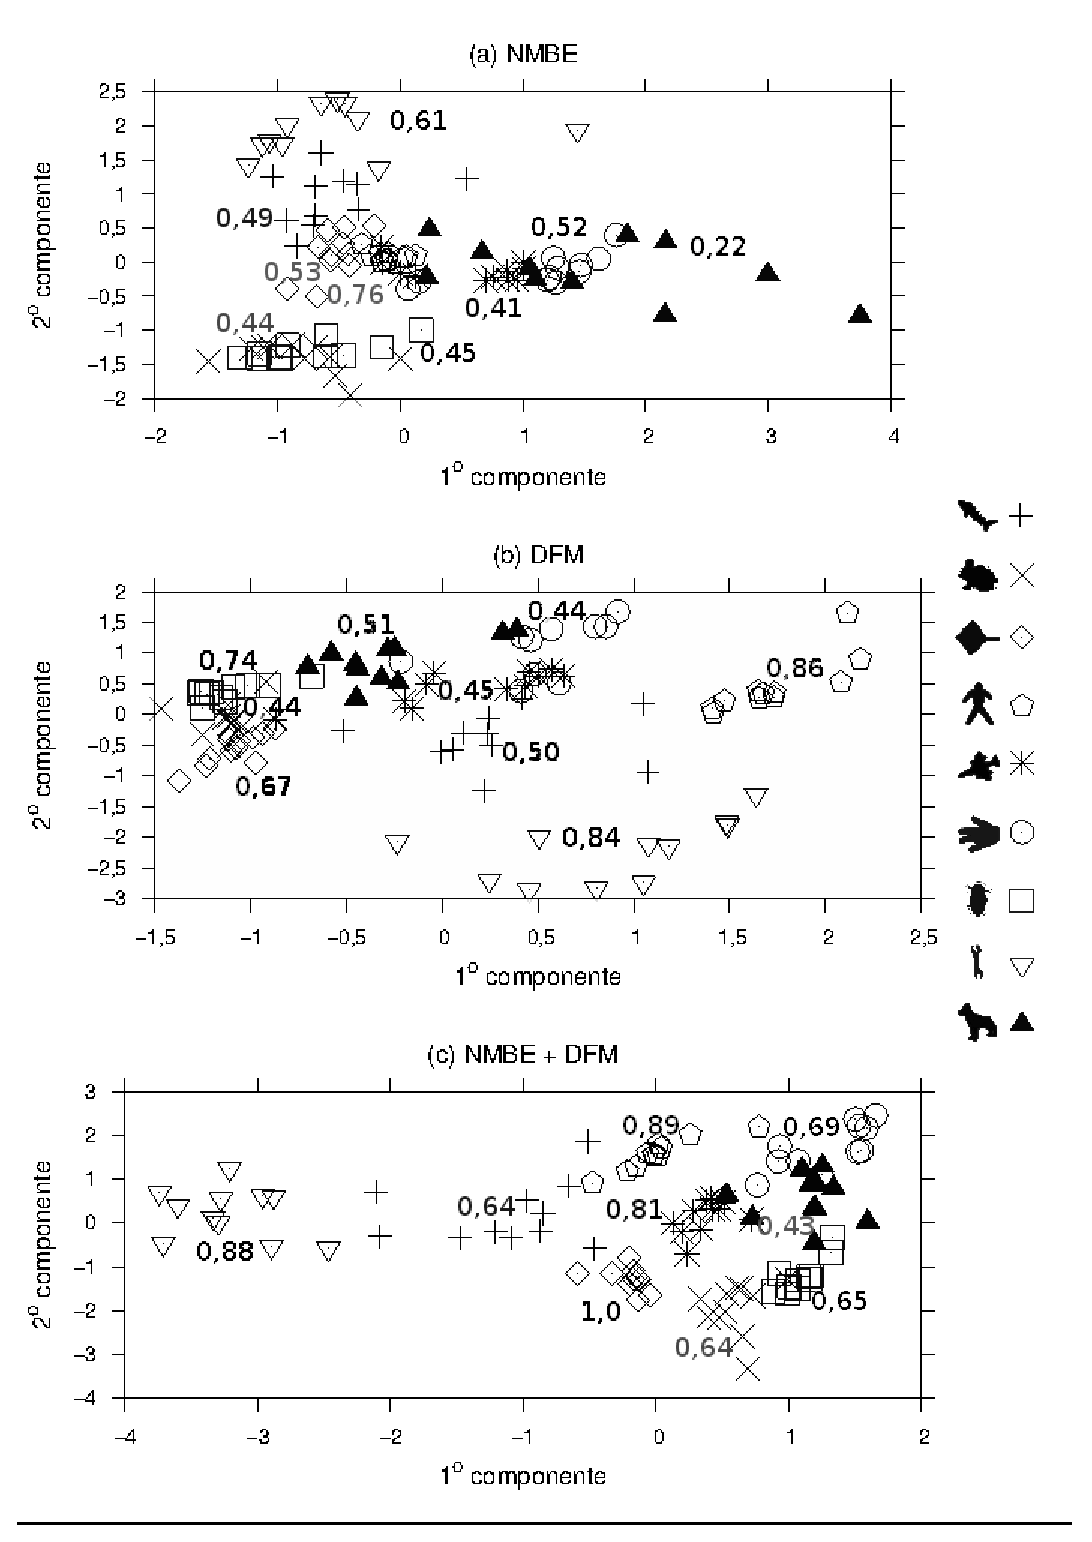
\includegraphics[width=0.75\textwidth]{nuvem_pca.eps}
\end{figure}

O propósito da análise das componentes principais é obter um conjunto de variáveis não correlacionadas, em ordem decrescente de importância, a partir da combinação linear das variáveis originais. Sob o aspecto geométrico, esse processo de combinar linearmente as variáveis pode ser entendido como realizar a rotação dos eixos do sistema de coordenadas original, a fim de se encontrar um novo sistema de coordenadas ortogonal em que as variáveis transformadas apresentem máxima variância. 

Desde que a maior parte da variância esteja concentrada nas primeiras componentes das variáveis transformadas, consegue-se obter através dessa técnica uma representação com um número reduzido de variáveis.

A técnica \emph{PCA} é não supervisionada, pois não leva em consideração informação a priori dos agrupamentos, ou rótulos, dos dados.  

Sendo a transformação \emph{PCA} linear, temos que

\begin{equation}\label{eq:PCA1}
\mathbf{y}=\mathbf{A}^T\mathbf{x}
\end{equation}

, aonde $ \mathbf{A} = \begin{pmatrix}
  a_{1,1} & a_{2,1} & \cdots & a_{p,1} \\
  a_{1,2} & a_{2,2} & \cdots & a_{p,2} \\
  \vdots  & \vdots  & \ddots & \vdots  \\
  a_{1,p} & a_{2,p} & \cdots & a_{p,p}
 \end{pmatrix} = 
 \begin{pmatrix}
 \mathbf{a_{1}}&
 \mathbf{a_{2}}&
 \cdots&
 \mathbf{a_{p}}
 \end{pmatrix}$ é a matriz de transformação, $\mathbf{x} = \begin{pmatrix} x_1&x_2&\ldots&x_p\end{pmatrix}^T$ e $\mathbf{y} = \begin{pmatrix}y_1&y_2&\ldots&y_p\end{pmatrix}^T$ vetores de variáveis aleatórias e $\mathbf{a_1}\text{ a }\mathbf{a_p}$ vetores dos coeficientes da base de transformação.
 
Logo, cada variável de saída $y_i$ é obtida através da combinação linear das variáveis de entrada pela seguinte equação:
 
 \begin{equation}\label{eq:PCA2}
 y_i = \sum\limits_{j = 1}^p a_{i,j}x_j = \mathbf{a_i}^T\mathbf{x}
 \end{equation}

Pode-se demonstrar que, para se obter em $\mathbf{y}$ variáveis que não são correlacionadas,  deve-se atribuir aos vetores de coeficientes $\mathbf{a_1} \ldots \mathbf{a_p}$ os auto-vetores da matriz de covariância de $\mathbf{x}$, sendo esta última dada por: 

\begin{equation}\label{eq:PCA3}
\mathbf{\Sigma_x} = E{[\mathbf{xx}^T]}-E{[\mathbf{x}]}E{[\mathbf{x}^T]}
\end{equation}

 aonde $E[.]$ denota o operador esperança. 
Já que $\mathbf{\Sigma_x}$ é de dimensão $p \times p$, temos associada a esta $p$ auto-vetores ($\mathbf{a_1}\text{, }\mathbf{a_2}\text{, }\ldots\text{, }\mathbf{a_p}$) com $p$ auto-valores ($\lambda_1 > \lambda_2 \ldots > \lambda_p$) correspondentes, sendo cada auto-valor $\lambda_i$ a variância de cada variável de saída $y_i$ obtida através da Equação \ref{eq:PCA2}. 

Selecionando dentre as componentes somente aquelas de maior variância, que implica em construir a matriz de transformação apenas com os auto-vetores mais significativos, é possível obter uma representação dos dados em um espaço de dimensão reduzida e de mais fácil entendimento do ponto de vista geométrico.

Na figura \ref{fig:nuvem_pca} temos representadas as projeções das duas componentes principais de maior variância para cada um dos descritores avaliados. Os valores numéricos correspondem a taxa de acerto média nos experimentos de recuperação de formas pelo conteúdo alcanças para cada classe de formas representada.

\subsection{Mapa auto-organizável de Kohonen}

O mapa auto-organizável de Kohonen, ou rede \emph{SOM} \cite{Kohonen:2001}, consiste em um tipo de rede neural de aprendizagem não supervisionada. Desenvolvida por \citeonline{Kohonen:1982}, a rede \emph{SOM} projeta os vetores apresentados em sua entrada de um espaço N-dimensional para um espaço bidimensional, preservando a estrutura topográfica do espaço vetorial de origem. Em outras palavras, se dois vetores encontram-se próximos no espaço de entrada, estes preservarão essa relação de proximidade no espaço de projeção. 

\begin{comment}
Em seu processo de treinamento, a rede \emph{SOM} agrupa os vetores de entrada através de um processo de aprendizado competitivo mantendo a estrutura topológica do espaço vetorial de entrada.
\end{comment}

Sendo uma ferramenta para análise exploratória de dados, esse tipo de rede neural tem sido empregada para visualização de imagens \cite{Strong2011774}, identificação de agrupamentos \cite{Kuroiwa200031}, classificação de texturas \cite{595364}, bem como outras aplicações.

\citeonline{Ultsch:1990} demonstraram que, embora a rede \emph{SOM} organize os vetores em agrupamentos, esta não representa as distâncias entre os mesmos de maneira fidedigna. Isso torna a análise direta do mapa de projeções não adequada para a análise dos agrupamentos estabelecidos. 

Para contornar esse problema, os referidos autores desenvolveram um método bidimensional de representação conhecido como matriz unificada de distâncias ou matriz-U. Obtida a partir do mapa \emph{SOM} essa matriz mostra, preservando a topologia, a relação de distância entre as estruturas mapeadas \cite{Ultsch:1990}. 

Para ilustrarmos como se interpreta a informação contida na matriz-U apresentamos como exemplo a imagem da Figura \ref{fig:u-matrix}. Nesta imagem a matriz-U é representada por um conjunto de células em níveis de cinza. As estruturas claras rotuladas representam os neurônios da rede SOM, enquanto as demais células representam o grau de separação existente entre as estruturas. Células mais escuras representam maior grau de separação entre as estruturas mapeadas pela matriz. Já células mais claras, tais como as que tendem ao branco, representam maior grau de proximidade entre as estruturas mapeadas. 

Interpretando esta figura observamos que as estruturas A5, A4 e A8 estão bem próximas umas das outras. Já a estrutura A9 encontra-se afastada das referidas estruturas. Dada a grande separação existente entre as quatro estruturas analisadas e as demais estruturas da matriz (E8, E6, E10, E9, E3 e B9), podemos inferir que as quatro estruturas (A5, A4, A8 e A9) formam um agrupamento. Já as estruturas E8, E6, E10 e E9 formam um outro agrupamento, embora não estejam tão próximas umas das outras como no caso anterior. Quanto às estruturas B9 e E3, estas estão isoladas, ou seja, muito distante das demais estruturas da matriz.


\begin{figure}[h!]
  \caption{\label{fig:u-matrix} Representação da Matriz-U como imagem em níveis de cinza. As células brancas rotuladas correspondem aos neurônios da rede SOM. Células escuras indicam maior separação entre neurônios e células claras indicam maior proximidade entre neurônios.}
  \centering
  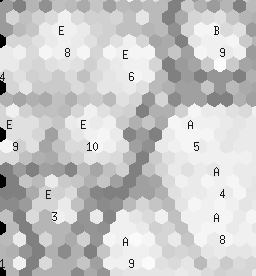
\includegraphics[width=0.5\textwidth]{u-matrix_gray.png}
\end{figure}


\section{Conceitos da teoria da informação}

Conceitos da teoria da informação têm sido aplicados, recentemente e com sucesso, em problemas de visão computacional e reconhecimento de padrões. Isso porque tais conceitos têm se mostrado apropriados para a modelagem do comportamento dos sistemas biológicos de percepção visual \cite{Escolano:2009}.

Grandezas como entropia e informação mútua também tem sido utilizadas como função custo no treinamento de sistemas adaptativos e de aprendizagem de máquina \cite{Principe:2011} pelo fato de terem relação direta com a informação contida nos sinais. Essas grandezas são expressas pelas funções densidade de probabilidade dos dados e que portanto devem ser estimadas. \citeonline{Principe:2010:ITL:1855180} sugere a janela de Parzen \cite{Webb:2002} como uma técnica conveniente para se estimar funções densidade de probabilidade. 



\subsection{Entropia de Shannon}

Na teoria da informação, a entropia de Shannon é uma medida do grau de incerteza que se tem, em média, dos possíveis estados que uma variável aleatória discreta pode assumir. Seja  $X$ uma variável aleatória discreta, que possa assumir $N$ diferentes valores $\{x_1\text{, } \ldots\text{ , }x_k\text{ , }\ldots\text{ , }x_N$\}, aonde a probabilidade de ocorrência de cada valor é $p_k = P(X = x_k) \text{,} \quad 0 \leq p_k \leq 1 \text{,} \quad \sum \limits_{k=1}^N p_k = 1$. A entropia de Shannon de $X$ é definida pela seguinte equação 

\begin{equation}\label{eq:Shannon}
H(X) = -\sum\limits_{k = 1}^N p_k\log{p_k}
\end{equation}

e apresenta as seguintes propriedades \cite{Thomas:2006}:

\begin{alineas}
\item $0 \leq H(X) \leq \log{N}$;  
\item $H(X) = 0$ se $p_k = 1$ para um único valor de $k$ e $p_k = 0$ para os demais valores de $k$;
\item $H(X) = \log{N}$ se $p_k = \frac{1}{N}$ para todos os valores de $k$.
\end{alineas}

A entropia de Shannon indica, em média, quanto de informação uma variável aleatória carrega. Quanto mais informativa uma variável aleatória é, maior o grau de surpresa que esta apresenta, ou seja, menos previsível é o seu valor.

\subsection{Entropia diferencial}

Para uma variável aleatória contínua $X$, com função densidade de probabilidade $p_X(x)$, a entropia diferencial é definida como sendo \cite{Thomas:2006}

\begin{equation}\label{eq:difent}
h(X) = -\int_{-\infty}^\infty p_X(x)\log{p_X(x)}dx\text{.}
\end{equation}

Essa definição é a extensão da entropia discreta de Shannon para o caso de variáveis aleatórias contínuas. No entanto, diferente da entropia de Shannon, a entropia diferencial não mede o grau de incerteza de $X$, pois tal incerteza é infinita, já que a quantidade de estados que um sistema contínuo pode realizar é infinita.

Considerando que uma variável aleatória contínua é o caso limite da variável aleatória discreta $X$, que assume valores $x_k = k \delta x$, $k = 0\text{, }\pm 1\text{, } \pm 2\text{, }\ldots$, quando $\delta x \mapsto 0$, demonstra-se que $H(X)$ e $h(X)$ guardam a seguinte relação \cite{Thomas:2006}:

\begin{equation} \label{eq:entropias}
H(X) = h(X) - \lim_{\delta x \mapsto 0}{\log{\delta x}}\text{.}
\end{equation}

A equação \ref{eq:entropias} evidencia que, à medida que $\delta x \mapsto 0 $, a entropia de Shannon, $H(X)$, tende a infinito. 

O problema associado com o termo $\log \delta x$ na equação \ref{eq:entropias} é contornado adotando-se $h(X)$ como sendo a entropia diferencial e considerando $-\log \delta x$ um fator de referência. Isso porque a informação processada por um sistema estocástico é obtida a partir da diferença entre duas medidas de entropias a partir de um referencial em comum. Desta forma, fica justificado o uso de $h(X)$ como uma medida de entropia para uma variável aleatória contínua.

A entropia diferencial apresenta a propriedade de ser invariante a translação da variável aleatória, ou seja:

\begin{equation}
h(X+a) = h(X)\text{.}
\end{equation}

No caso de mudança da escala da variável aleatória por um fator $\alpha$, temos a seguinte propriedade:

\begin{equation}\label{eq:escala_entropia}
h(\alpha X) = h(X) + \log{\alpha}\text{.}
\end{equation}

\subsection{Medidas de divergência}

Um problema recorrente em reconhecimento de padrões e processamento de sinais é a determinação do grau de similaridade entre dois conjuntos de dados. Considerando que esses conjuntos de dados são realizações de duas variáveis aleatórias, pode-se avaliar tal similaridade comparando-se os modelos estatísticos que as descrevem entre si, sendo as medidas de divergência uma ferramenta apropriada para esse fim. 

Com aplicação em probabilidade e estatística, processamento de sinais, reconhecimento de padrões e teoria da informação, medidas de divergência determinam o quão diferentes são duas distribuições de probabilidade. 

Temos na tabela \ref{tbl:cont_div} as expressões matemáticas para o cálculo de algumas medidas de divergência. Essas derivam de uma família de funções que foram definidas por Csiszár e que recebem o nome de funções f-divergentes \cite{1999880}. 

Sendo $p$ e $q$ distribuições de probabilidade, com domínio em $x$, definem-se as funções f-divergentes como sendo

\begin{equation}
D_f(p,q) = \int_xqf(\frac{p}{q})dx\text{,}
\end{equation}

aonde $f:(0,\infty)\mapsto\mathbb{R}$ é uma função convexa.


Assim, para se calcular as medidas de divergência, é necessário estimar as funções densidade de probabilidade que melhor descrevem os conjuntos de dados a partir de amostras. Duas abordagens podem ser empregadas para esse fim: a paramétrica e a não paramétrica.

Na abordagem paramétrica assume-me que as variáveis aleatórias seguem leis de probabilidade cujas funções densidade de probabilidade são analiticamente conhecidas. Desta forma, o problema consiste em determinar os parâmetros dessas funções densidade de probabilidade a partir dos dados amostrais. 

A vantagem de se estimar funções de densidade através da abordagem paramétrica é a possibilidade de se obter soluções analíticas fechadas para as medida de divergência. O problema é que nem sempre consegue-se estimar satisfatoriamente os parâmetros da lei de probabilidade a partir dos dados amostrais disponíveis. Ademais, dependendo da lei de probabilidade assumida, muitas vezes não se consegue encontrar uma expressão analítica fechada que permita o cálculo da medida de divergência desejada.

Já na abordagem não paramétrica, nenhuma lei de probabilidade analítica é assumida, sendo a função densidade de probabilidade estimada, diretamente, a partir dos dados amostrais. Diversas técnicas podem ser empregadas na abordagem não paramétrica para se estimar a função densidade, tais como histogramas, k-vizinhos próximos e janela de Parzen.  

\begin{table}
\centering
\caption{\label{tbl:cont_div}Medidas de divergência entre funções de distribuição de probabilidade}
\begin{tabular}[]{ll}
\hline
Medida de divergência&Fórmula matemática\\
\hline
Divergente de Kullback-Leibler&$d_{KL}(p,q) = \int_{x} p\log{\frac{p}{q}}dx$\\
Divergente de Jensen-Shannon&$d_{JS}(p,q) =\frac{1}{2}d_{KL}(p,h)+\frac{1}{2}d_{KL}(q,h)$, $h = \frac{p+q}{2}$\\
Divergente de Patrick Fisher&$d_{PF}(p,q) = \sqrt{\int_{x}{(p-q)}^2dx}$\\
Chi-square&$d(p,q)= \int_{x}{\frac{(p-h)^2}{h}dx}$,$h = \frac{p + g}{2}$\\
Chernoff&$\displaystyle d(p,q) = - \min_{0<\alpha<1}{log{\int_{x}{p^{\alpha}q^{1-\alpha}}dx}}$\\
Bhattacharyya&$d(p,q) = -2log{\int_{x}{\sqrt{pq}dx}}$\\
Hellinger&$d(p,q)=\frac{1}{\sqrt{2}}\sqrt{\int_{x}{(\sqrt{p}-\sqrt{q})^2dx}}$\\
Divergente de Rényi&$d_{\alpha}(p,q) =\frac{1}{\alpha-1}\log{\int_{x}{p^{\alpha}q^{1-\alpha}}dx}$\\
\hline
\end{tabular}
\end{table}


\begin{table}
\centering
\caption{\label{tbl:divergence}Medidas de divergência entre distribuições de probabilidade de massa}
\begin{tabular}[]{ll}
\hline
Medida de divergência&Fórmula matemática\\
\hline
Divergente de Kullback-Leibler&$d_{KL}(p,q) = \sum\limits_{i = 1}^{n} p_{i}\log{\frac{p_{i}}{q_{i}}}$\\
Divergente de Jensen-Shannon&$d_{JS}(p,q) =\frac{1}{2}(d_{KL}(p,h)+d_{KL}(q,h))$, $h = \frac{p+q}{2}$\\
Divergente de Patrick Fisher&$d_{PF}(p,q) = \sqrt{\sum\limits_{i=1}^{n}{(p_i-q_i)}^2}$\\
Chi-square&$d(p,q)= \sum\limits_{i = 1}^{n}{\frac{(p_{i}-h_{i})^2}{h_{i}}}$, sendo $h_{i} = \frac{p_{i} + g_{i}}{2}$\\
Chernoff&$\displaystyle d(p,q) = - \min_{0<\alpha<1}{log{\sum\limits_{i=1}^{n}{p_i^{\alpha}q_i^{1-\alpha}}}}$\\
Bhattacharyya&$d(p,q) = -2log{\sum\limits_{i = 1}^{n}{\sqrt{p_{i}q_{i}}}}$\\
Hellinger&$D_{H}=\frac{1}{\sqrt{2}}\sqrt{\sum\limits_{i = 1}^{n}{(\sqrt{p_{i}}-\sqrt{q_{i}})^2}}$\\
Divergente de Rényi&$d_{\alpha}(p,q) =\frac{1}{\alpha-1}\log{\sum\limits_{i = 1}^{n}{p_i^{\alpha}q_i^{1-\alpha}}}$\\
\hline
\end{tabular}
\end{table}


Se $X\text{ e }Y$ são variáveis aleatórias discretas, ambas podendo assumir um conjunto de valores $\chi \in \{x_{1},x_{2},x_{3},\ldots,x_{n}\}$, então suas densidades de probabilidade de massa são $p = (p_{1},p_{2},\ldots,p_{n})$ e $q = (q_{1},q_{2},\ldots,q_{n})$ respectivamente, aonde $p_i = Pr(X = x_{i})$ e $q_i = Pr(Y = x_{i})$.    

Com base nessas definições apresentamos na tabela \ref{tbl:divergence} as versões discretas dos divergentes da tabela \ref{tbl:cont_div}.

\begin{comment}
From Sample Similarity to Ensemble
Similarity: Probabilistic Distance Measures
in Reproducing Kernel Hilbert Space


Probabilistic distance measures find use in many research
areas such as probability and statistics, pattern recognition,
information theory, communication, and so on. In statistics,
the probabilistic distances are often used in asymptotic
analysis. In pattern recognition, pattern separability is
usually evaluated using probabilistic distance measures [1],
[2] such as Chernoff or Bhattacharyya distances because they
provide bounds for the probability of error. 
\end{comment}


%Isso porque embora duas formas estejam numa mesma classe, estas podem ter variações substanciais em suas características de baixo nível, e mesmo assim serem consideradas similares apesar da distância entre as mesmas ser significativas.


%\subsection{Divergente de Kullback-Leibler}
O divergente de Kullback-Leibler (KL), também conhecido como entropia relativa, não corresponde a uma métrica de distância por não ser simétrica e por não respeitar a propriedade de desigualdade triangular. No entanto, demonstra-se que a mesma é sempre positiva, sendo igual a zero se e somente se $p = q$.

Outra característica importante do divergente de KL é que seu valor não apresenta um limite superior. Isso porque se, para algum valor de $i$, $p_{i} = 0$ e $q{i} \neq 0$, $D_{KL}(p,q) \to \infty$.

Esse divergente é de grande importância na teoria da informação, já que a informação mútua, que é um caso particular do divergente de KL, é uma medida da capacidade de um canal de comunicação \cite{Thomas:2006}. Ademais, o divergente de KL é utilizado como função custo em aplicações de filtragem adaptativa e na seleção de sinais.  

%\subsection{Divergente de Jensen-Shannon}

O divergente de Jensen-Shannon (JS) é construído a partir do divergente de KL. Embora apresente a propriedade de simetria, este divergente não respeita a propriedade de desigualdade triangular. A faixa de valores que o divergente de JS  pode assumir é delimitada entre $0$ e $1$ no caso de o logaritmo da Equação do divergente de KL ser $2$.
 
\begin{comment}
$D_{JS}(p,q) =\frac{1}{2}(D_{KL}(p,h)+D_{KL}(q,h))$, sendo $h = \frac{p+q}{2}$
\end{comment}

%\subsection{Patrick Fisher}

O divergente de Patrick Fisher foi originalmente proposto em \citeonline{1054354} como uma função custo a ser maximizada na seleção não paramétrica de características. Em \cite{662771}, esse é utilizado como uma função custo a ser otimizada num método não paramétrico de obtenção de um discriminante linear.  

\begin{comment}
$D_{PF}(p,q) = \sqrt{\sum\limits_{i=1}^{n}{(p_i-q_i)}^2}$
\end{comment}

%\section{Chi-square}
%$D_{CS}(p,q)= \sum\limits_{i = 1}^{n}{\frac{(p_{i}-h_{i})^2}{h_{i}}}$, sendo $h_{i} = \frac{p_{i} + g_{i}}{2}$

\begin{figure}[h!]
  \caption{\label{fig:graph2} Gráficos ilustrando os valores das divergências entre as distribuições de probabilidade de massa $(p\quad1-p)\text{, } p \in [0,1]$ e $(0,5\quad0,5)$.}
  \centering
  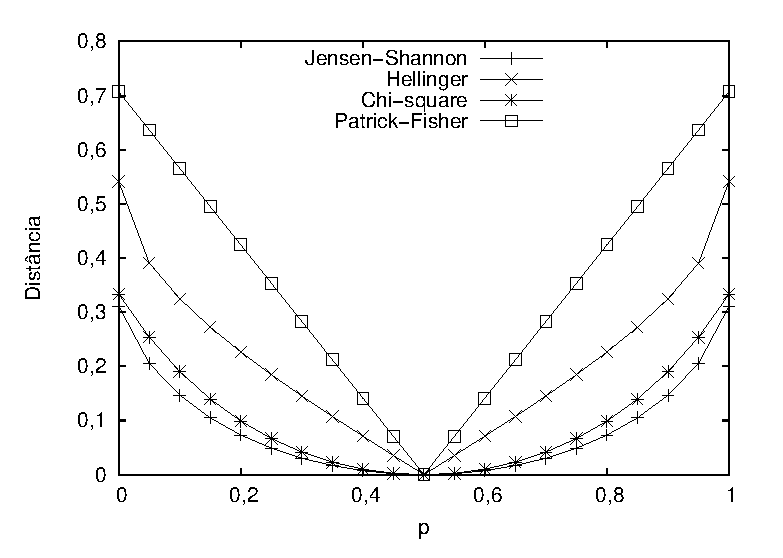
\includegraphics[width=0.75\textwidth]{graph2.eps}
\end{figure}

%\subsection{Divergente de Rényi}
O divergente de Rényi generaliza algumas das medidas de divergência apresentadas até então.

%$D_{\alpha}(p,q) =\frac{1}{\alpha-1}\log{\sum\limits_{i = 1}^{n}{p_i^{\alpha}q_i^{1-\alpha}}}$

%\subsection{Chernoff}
%$\displaystyle D_C(p,q) = - \min_{0<\alpha<1}{log{\sum\limits_{i=1}^{n}{p_i^{\alpha}q_i^{1-\alpha}}}}$

%\subsection{Bhattacharyya}
%$D_{B}(p,q) = -2log{\sum\limits_{i = 1}^{n}{\sqrt{p_{i}q_{i}}}}$

%\subsection{Hellinger}
%$D_{H}=\frac{1}{\sqrt{2}}\sqrt{\sum\limits_{i = 1}^{n}{(\sqrt{p_{i}}-\sqrt{q_{i}})^2}}$

\begin{comment}

The concept of fractal, introduced by Mandelbrot \citep{Mandelbrot:2000}, is closely related to self-similarity or scaling of a shape. Moreover, it encompasses the notion of fractional dimension.  Actually, fractal dimension and \emph{MFD} are well-known methods to estimate shape complexity \citep{Backes:2012}. Shape complexity is an important concept in shape analysis that informs how much space a shape occupies \cite{Costa:2009}. \emph{MFD} estimates shape complexity through a curve that represents changes in the complexity as the shape visualization scale varies \cite{Florindo:2012}. 

%and for feature extraction of biological forms %\citep{Rossatto:2011}.  In fact, it quantifies the %self-similarity of a shape.

% quantifica a aspereza ou rugosidade de uma forma \citep{Schroreder:1996}.\\

%Uma das caracter\'isticas das formas fractais \'e a sua auto-similaridade \citep{Schroreder:1996}. Isso significa que uma forma, tanto em escalas menores como maiores, \'e constitu\'ida por um mesmo conjunto de primitivas $D_f$.\\

%Qualquer forma auto-similar pode ser dividida em $N$ partes auto-similares, ou seja, c\'opias menores que sejam escalonadas por um fator $b$, atrav\'es da equa\c c\~ao:\\

%\begin{equation}
%D_{f} = \frac{\log{N}}{\log{\frac{1}{b}}}.
%\label{eq:dfc}
%\end{equation}

%Esse descritor pode ser construído a partir do método de Bouligand-Minkowski de estimação da dimensão fractal ($D_f$) \citep{Costa:2009}. Utilizado em \citep{Florindo:2012} e \citep{Backes:2012}, o referido método aplica dilatações exatas à  forma analisada tendo como elemento estruturante uma região circular de raio $r > 0$. O coeficiente angular da interpolação linear da curva $\log{A(r)}$ versus $\log{r}$ é utilizado como uma estimativa da $D_f$:

In this paper, the Minkowski-Bouligand method estimates the fractal dimension ($D_f$) \citep{Costa:2009} and hence the \emph{MFD} descriptor. This estimation method dilates the shape under analysis  using a disk structuring element of radius $ r>0 $, successively. The slope of the linear interpolation of the curve $\log{A(r)}$ versus $\log{r}$ provides the $D_f$ estimation, given by: 

\begin{equation}
D_f = 2 - \lim_{r \to 0}  \frac{\log{A(r)}}{\log{r}}.
\label{eq:df}
\end{equation}
%O cálculo da MFD decorre do calculo da derivada da curva log-log, obtida a partir da equação \ref{eq:df}, para diferentes valores de raios $r$:
Then, the derivative of th log-log curve for $N$ discrete values of radii $r_i>0$ gives 

\begin{equation}
MFD = \big(D_f(t_1)\text{, }D_f(t_2)\text{, }\ldots\text{ , }D_f(t_N)\big), 
\label{eq:dfm}
\end{equation}

\noindent where  $D_f(t) = 2 - \frac{du(t)}{dt}$, $t = \log{r}$ and $u(t) = \log{A(t)}$.

\end{comment}
% !TeX root = ../main.tex
\chapter{Conclusões e Trabalhos Futuros \label{chap:ch5}}

Esta tese abordou a caracterização e análise de formas por meio de descritores multiescala baseados em conceitos de curvatura como a energia de dobramento. Estes descritores foram calculados a partir do contorno de formas binárias de bases de uso geral e uma base pública de folhas. Considerando que estes descritores podem ser utilizados em diferentes aplicações de visão computacional e,  portanto, distintas bases de imagens, introduzimos uma metodologia versátil de ajuste automático de parâmetros por otimização evolucionária. 

Vale destacar a importância e ao mesmo tempo a dificuldade inerente ao processo de ajuste manual ou empírico de parâmetros multiescala a um determinado problema ou aplicação. Assim sendo, neste trabalho apresentamos uma alternativa automática para o delineamento do descritor e seus parâmetros às particularidades do problema e da base em estudo.  
Além disso, a alternativa do ajuste automático se destaca por não ser fatigante como o ajuste manual arbitrário ou empírico.

Na metodologia proposta para análise de formas de folhas de plantas, a função objetivo, a ser minimizada no processo de busca dos parâmetros, é fundamentada na medida de qualidade de agrupamento \textit{silhouette}. Como resultado da minimização desta função objetivo, encontramos um conjunto otimizado de parâmetros de escala dos descritores de forma que são utilizados na análise de formas, em particular, de folhas de plantas.  

A versatilidade desta metodologia se deve, portanto, ao fato de que a mesma pode ser ajustada à função  objetivo ou função custo e moldada assim para as bases de imagens do problema abordado. Ademais, seu desempenho se mostrou satisfatório e promissor, uma vez que os parâmetros otimizados incorporaram características e detalhes sutis das formas, o que foi confirmado pelas técnicas de avaliação qualitativa e quantitativa. 

De fato, o conjunto otimizado de parâmetros, moldados pela minimização da função objetivo,  embute informações de nuances da forma. A comprovação desde achado se deu pela considerável melhoria alcançada na organização dos agrupamentos, quantificada pela medida da qualidade de agrupamento e pela elevação na taxa de acerto da classificação das formas ao utilizarmos os descritores otimizados em bases com elevada similaridade de formas entre classes. 

As versões otimizadas dos descritores estudados discriminaram diferenças de formas dentro de uma mesma classe e entre classes. Observamos ainda que determinadas classes de formas apresentaram-se mais desafiadoras que as demais para a representação das mesmas, e isso foi comprovado pela medida \textit{silhouette}  e o arranjo espacial exibido pelas técnicas de visualização exploratória de agrupamentos.

Experimentos com uma base pública de imagem de folhas indicaram a adequação das metodologias propostas em problemas de taxonomia de folhas de plantas. Vale ressaltar que a base de imagens de folhas de plantas Flavia é bastante desafiadora pois a mesma apresenta uma elevada similaridade entre formas de classes distintas. Isso significa que formas de classes distintas não apresentam significativas variações nos contornos das mesmas. Entretanto, essas particularidades podem ser captadas pelos descritores multiescala, os quais se mostraram bastante efetivos no agrupamento e classificação de formas de folhas.
Esta importante característica da base Flavia é portanto um desafio para a metodologia e  para os descritores, de modo geral. 

Logo, a metodologia proposta constitui uma ferramenta adicional e fonte de informação para taxonomistas discriminarem e agruparem espécies de plantas. 


\section*{Trabalhos futuros}
Deste trabalho, se desdobram outras ações futuras relacionadas a seguir: 
\begin{itemize}

\item melhoria do processo de otimização dos parâmetros, buscando outras alternativas para a função objetivo, de modo que se reduza o custo computacional da metodologia e melhore as taxas de classificação e recuperação;

\item análise de desempenho da metodologia proposta em outros problemas de visão computacional como reconhecimento automático de células saudáveis e com carcinoma a partir de descritores multiescala de formas;

\item aplicação da metodologia de otimização em classificação taxonômica de outras espécies vegetais e animais;

\item investigação e ajuste dos parâmetros dos algoritmos de otimização de modo que resultem em maior estabilidade na convergência, assim como em maior velocidade de processamento;

\item seleção e testes de outros algoritmos de otimização evolucionária em análise  de formas.

\end{itemize}

\begin{comment}
\textcolor{red}{
In this paper, we introduce a promising methodology for a multiscale descriptor evaluation and used it to investigate the suitability of \emph{NMBE} and \emph{MFD} shape descriptors for CBIR applications. Thus, 
this methodology can be used to evaluate and select shape descriptors for a specific CBIR application.

Our experiments showed that the proposed descriptor can reliably retrieve shapes that exhibit multiscale characteristics similar to those of a given query image. Moreover, the \emph{NMBE} was more robust in distinguishing subtle shape differences within classes than \emph{MFD}.

The relationship between these descriptors and the classes of binary shapes that they represent in a multidimensional space was inferred using the U-matrix. Our findings established that this high-dimensional projection tool provides a qualitative evaluation and visual explanation of how the different classes of shapes are spatially grouped and scattered. Regarding the methodology for quantitative evaluation,  we concluded that the \emph{Silhouette} measure was suitable and fair in numerically assessing the performance of multiscale descriptors and thus inferring  whether a descriptor was able to represent a shape in CBIR applications. 
The qualitative and quantitative evaluation approaches provide valuable information to help elucidate how descriptors represent shapes in a multidimensional space, and therefore we recommend these methods for CBIR experiments.


%\color{red}
We have also investigated  a theoretical relationship between these descriptors and the classes of objects in two public databases of binary images within a multidimensional space by using the U-matrix. Our findings have shown that the high dimensional projection tool, i.e., U-Matrix (SOM map) provides a qualitative evaluation and visual explanation of how the different classes of shapes are spatially grouped or scattered. Regarding the methodology for quantitative evaluation,  we concluded that the \emph{Silhouette} measure was suitable to numerically assess the performance of the multiscale descriptors and thus infer  whether a descriptor is able or not to represent a shape in CBIR applications. 
In fact, the qualitative and quantitative evaluation approaches provided valuable information to help understand how descriptors represent shapes in a multidimensional space.
%\color{black}


The \emph{NMBE} descriptor arises from the bending energy calculated for a shape contour submitted to several stages of smoothing.  Highly discriminating features contribute towards obtaining high clustering or classification accuracy.\color{black} 
This results in a shape signature that allows the use of classical similarity measures at low computational cost.
Since that only the euclidean $L_2$ norm was used as distance metric in our evaluation proposal, we expect to adapt it to other metrics in a future work. 

The CBIR algorithms that were developed can reliably retrieve the candidate image patches exhibiting intensity and morphological characteristics that are most similar to a given query image. The methods described in this paper are able to reliably discriminate among subtle staining differences and spatial pattern distributions. By integrating a newly developed dual-similarity relevance feedback module into the CBIR framework, the CBIR results were improved substantially. By aggregating the computational power of high performance computing (HPC) and cloud resources, we demonstrated that the method can be successfully executed in minutes on the Cloud compared to weeks using standard computers. 

to improve the shape retrieval performance and, furthermore, Figure \ref{fig:descritores}b the weak discriminating property of \emph{MFD}
are more spaced than the ones observed in Figure \ref{fig:descritores}b. Accordingly, the corresponding shapes appears in the U-matrix more scattered for \emph{MFD} than for \emph{NMBE}. Thus, it illustrates how \emph{NMBE} tends to improve the retrieval performance and, furthermore, the weak discriminating property of \emph{MFD}.


In this paper, we used the Euclidean $L_2$ norm, but future research will investigate other distance metrics. 

In this work we propose a method to evaluate similarity between binary shapes by employing divergence measures and combination of shape contour signatures. Finally, our tests led us to conclude that:  a) divergence measures are promising tools for shape similarity evaluation in shape retrieval; b) divergences that present high sensitivity to small variations between similar mass distributions tend to perform worst in shape similarity evaluation than divergences that feature low sensitivity and c) combining different shape signatures improves the shape retrieval Precision in experiments. 

This paper presents an optimization methodology for parameter adjustment of shape descriptors applied to leaf characterization and clustering. Our optimization methodology is a versatile tool for shape analysis that mainly relies on an objective function that can be adapted to different application problems or databases. Here, the minimization of the objective function accomplishes the best parameter set of a given shape descriptor to improve leaf characterization quality. 

The performance evaluation of the optimization methodology led us to conclude that the optimized parameters were able to reveal subtle leaf shape features and overall they have improved cluster organization and classification of plant leaves.
Actually, the optimized descriptors have reliably characterized shapes that exhibited multiscale features and they have also discriminated shape differences within and among leaf classes.
Likewise, the optimized shape descriptors provided a global and robust description on the challenging Flavia data set,  despite it presents a high between class similarity.

A relevant visual analysis of the proposed methodology linked the optimized and non-optimized NMBE with the classes of binary shapes that they represented in a multidimensional space by using U-matrices. This high-dimensional projection tool provided a qualitative evaluation and visual explanation on how the different classes of shapes were better spatially grouped and scattered due to the optimization methodology. Regarding the quantitative performance evaluation,  we have also observed that the \emph{silhouette} measure was suitable to numerically assess the multiscale shape descriptor and thus infer whether it was able to characterize leaf shapes or not. Our findings indicated that the optimized NMBE and IDSC were suitable to characterize leaf shapes and furthermore they may provide shape signatures to address leaf  taxonomy problems. Moreover, the proposed methodology is an additional tool and source of information for plant taxonomist to discriminate and group leaf species.
}
\end{comment}
\chapter{Metodologia}
\label{chap:MatMet}

O Capítulo \ref{chap:FUNDA} apresentou alguns dos métodos encontrados na literatura para a representação computacional de formas a partir do seu contorno.  Em muitos casos, esses métodos apresentam parâmetros que requerem ajustes, sendo esse ajuste dependente da natureza da aplicação, ou seja,  das características da base de imagens e do propósito ao qual o sistema de reconhecimento se destina. A energia de dobramento multiescala, por exemplo, requer o ajuste do número e os valores dos fatores de escala utilizados na representação das formas. 

Esse capítulo apresenta um método robusto e versátil para o ajuste desses parâmetros para customizar esses descritores em aplicações de classificação supervisionada e não supervisionada.   
 

%Os descritores entropia multiescala, apresentado no Capítulo \ref{chap:FUNDA}, e a energia de dobramento multiescala requerem o ajuste dos seguintes parâmetros: o número e os valores dos fatores de escala utilizados na representação das formas. Esse capítulo apresenta um método robusto e versátil para o ajuste desses parâmetros para customizar esses descritores em aplicações de classificação supervisionada e não supervisionada.   
 

\section{Ajuste de parâmetros}
A metodologia para escolha de parâmetros do descritor segue o esquema da Figura \ref{fig:Avaliacao}. Essa metodologia melhora a representação do descritor utilizando métodos de otimização evolutivos para minimizar uma função custo que corresponde a mediana do erro absoluto da silhouette dos descritores ($MAD$). O que motivou a escolha dessa função custo é sua robustez a valores extremos \cite{Rousseeuw:1987:2}, sendo sua equação 

\begin{equation}
\label{eq:mad}
MAD = \operatorname{mediana}\big(|s_i - 1|_{i =1,\:2,\:\cdots,\:L}\big)\text{,}
\end{equation}

\begin{figure*}[ht]
\centering
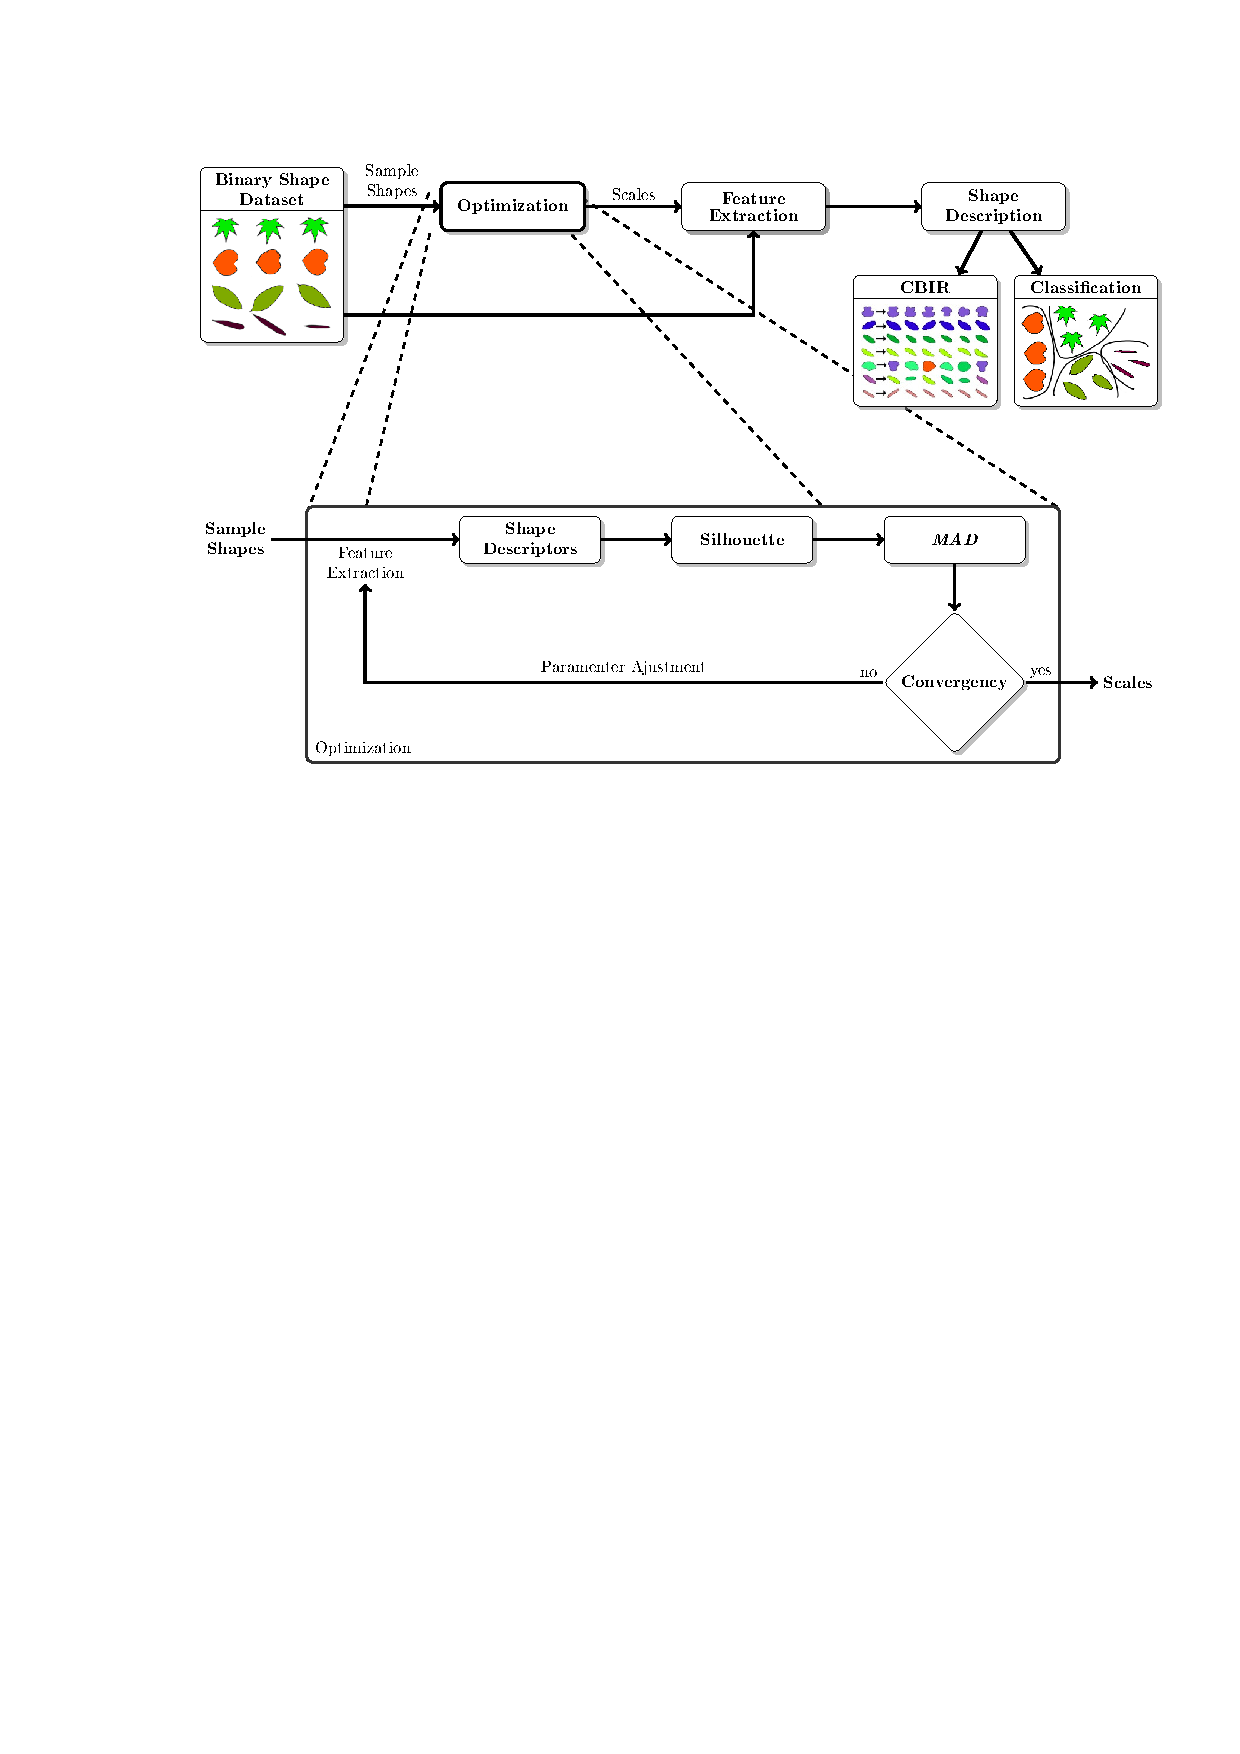
\includegraphics[width=\textwidth,trim = 14mm 164mm 0mm 24mm,clip]{Final_Flux.pdf}
\caption{Proposta de uma metodologia para otimização evolucionária de um descritor multiescala de forma.} 
\label{fig:Avaliacao}
\end{figure*}

\noindent aonde $S = \{s_1,s_2,\cdots,s_L\}$ é o conjunto das \emph{silhouettes} calculadas para $L$ descritores de forma. Os operadores $|.|$  e {$mediana ( )$} retornam o valor absoluto e a mediana de um conjunto de valores, respectivamente.

A Silhouette \cite{Rousseeuw:1987} é uma medida de qualidade de agrupamentos que indica o grau de afinidade de uma amostra  a um agrupamento, levando em conta as distâncias médias entre-classes e intra-classes de um objeto $i$ atribuído a uma dada classe $A$. Logo, esta métrica é definida como 
\begin{equation}
s_i = \frac{b_i - a_i}{\max{(a_i,b_i)}} \in [-1,1],
\end{equation}

\noindent sendo $a_i$ a dissimilaridade média entre o objeto $i$ e os demais objetos pertencentes a mesma classe de $a_i$ e $b_i$ é a dissimilaridade média do objeto $i$ e a classe vizinha mais próxima de $i$, excluída sua própria classe. 

Essa métrica pode assumir valores no intervalo $[-1,1]$, sendo que valores negativos indicam que o grau de pertencimento de um objeto à classe que este fora atribuído é baixo. Já valores positivos indicam que o grau de pertencimento de um objeto à classe que este fora atribuído é alto. Um valor de silhouette próximo de zero indica que o objeto está na fronteira entre duas classes e que há, portanto, um grau de incerteza a respeito de qual classes este pertence.

Os valores da função objetivo $MAD$ assume valores no intervalo $[0,2]$. De forma análoga a silhouette, um valor igual a zero desta função indica que a estrutura dos clusters é perfeita, enquanto que valores próximos de $2$ indicam que a estrutura dos clusters é deficiente, com baixa similaridade entre os objetos de mesma classe ou alta similaridade entre os objetos de classes distintas.

A Figura  \ref{fig:Avaliacao} ilustra, em detalhes, como se dá o ajuste dos parâmetros do descritor multiescala dentro da metodologia proposta, bem como esta avalia a qualidade do descritor obtido com os parâmetros otimizados.  Primeiramente, é amostrado na base de folhas um sub-conjunto das formas para, em seguida, realizar o procedimento de otimização e encontrar o melhor conjunto de parâmetros de escala  $\boldsymbol{\sigma}_{otim} = (\sigma_1,\:\sigma_2,\:\cdots,\:\sigma_k)$ do descritor multiescala que minimize a função custo da Equação \ref{eq:mad}. Então, utilizando-se as escalas encontradas realiza-se, com o descritor multiescala, a extração de características de toda a base de folhas.

O desempenho do descritor, em termos de agrupamento das formas, é avaliado qualitativamente e quantitativamente. Na avaliação qualitativa dois algoritmos de visualização de dados são utilizados: o mapa auto-organizável de Kohonen \cite{Kohonen:2001} e o \textit{multidimensional scaling} \cite{cox:2000}. Esses algoritmos produzem projeções bi-dimensionais das descrições das formas da base de folhas, provendo uma representação gráfica que possibilita a análise da qualidade dos agrupamentos. Assim, consegue-se inferir o quão eficaz o descritor é em organizar espacialmente as formas. Já na avaliação quantitativa são analisadas métricas de avaliação obtidas em experimentos de classificação supervisionada (precisão e revocação), de recuperação de formas (bulls-eye) e a medida silhouette \cite{Rousseeuw:1987} média por classe. 

A silhouette média por classe avalia tanto a coesão como a separação das classes através da distância entre os vetores de características. Já as métricas de precisão e revocação são medidas clássicas na avaliação do desempenho de descritores em experimentos de classificação supervisionada. Na classificação supervisionada, os classificadores utilizados foram Naive Bayes (NB) \cite{Fukunaga:1990}, \emph{K}-vizinhos próximos (Knn, $K = 5$) \cite{Fukunaga:1990,Webb:2002},  o discriminante linear de Fisher (LDA) \cite{Webb:2002} e o discriminante quadrático (QDA) \cite{Fukunaga:1990}.  Antes da classificação com os classificadores NB e \emph{Knn} foi utilizado o discriminante linear de Fisher para transformar os dados \cite{Webb:2002}. Já para classificação com os classificadores LDA e QUA aplicou-se a análise das componentes principais para descorrelacionar os dados. Os experimentos realizados de recuperação de imagens pelo conteúdo visam avaliar o desempenho dos descritores de formas e das medidas de similaridade estudadas neste trabalho. As metodologias utilizadas nesses experimentos são as mesmas encontradas em diversos trabalhos de recuperação de formas da literatura.

Foram realizados experimentos em duas bases de imagens de formas binárias: a Kimia, de 99 formas, e a MPEG-7 CE-Shape-1 de 1400 formas. Ambas as bases estão apresentadas no Apêndice deste trabalho.

A  Figura \ref{fig:metodo_cbir} ilustra a metodologia dos experimentos de recuperação de formas.  Primeiramente realiza-se a extração de características das formas da base de imagens de formas binárias com o método de descrição sob avaliação. O mesmo processo de extração de características é aplicado a imagem de uma forma de consulta. Esse processo resulta numa base de dados com os vetores de características associados às formas utilizadas no experimento. 

Com a medida de similaridade avalia-se o grau de correspondência existente entre o vetor de características da forma de consulta e os vetores associados a cada uma das formas da base. Tem-se assim como resultado uma lista de imagens recuperadas em ordem decrescente de similaridade à forma de consulta. Todo esse processo é realizado repetidamente tomando-se cada forma da base de imagens como forma de consulta e recuperando-se as demais.

\begin{figure}[h!]
  \caption{\label{fig:metodo_cbir} Metodologia empregada para os experimentos de recuperação de formas pelo conteúdo.}
  \centering
  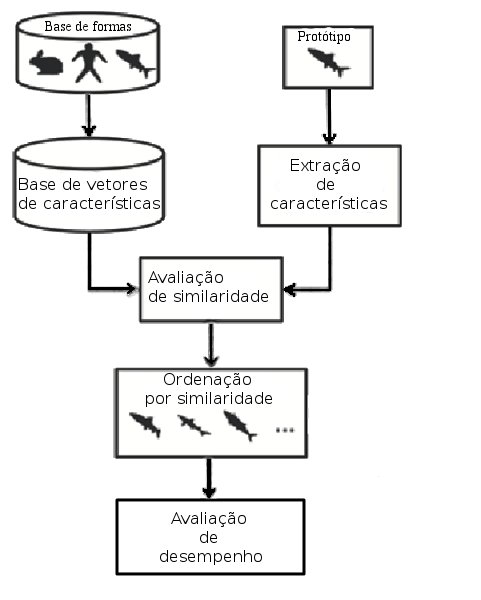
\includegraphics[width=0.55\textwidth]{Metodologia1.jpg}
\end{figure}

Na avaliação do desempenho dos experimentos duas medidas são utilizadas: o número total de acertos por posição recuperada e a medida Bull-eye.

A primeira medida consiste no número total de ocorrências de formas da mesma classe que a forma de consulta em cada posição recuperada.  Em diversos trabalhos de recuperação de formas pelo conteúdo o número total de acertos por posição recuperada é calculado para a base Kimia-99 \cite{Bernier:2003}. Tendo esta base 99 formas, igualmente distribuídas em 9 classes, são realizadas 99 recuperações das 11 formas mais similares à imagem de consulta. Como resultado espera-se obter um total de 99 formas recuperadas corretamente para cada posição recuperada.

A medida Bulls-eye também é utilizada na literatura para a comparação de diferentes métodos de recuperação de formas. Essa medida é calculada para a base MPEG-7 CE-Shape-1 da seguinte maneira: tomando-se cada forma dessa base de imagens como elemento de consulta, contabiliza-se o número de recuperações pertencentes a mesma classe da forma de consulta dentre as 40 primeiras posições recuperadas. Como resultado calcula-se a percentagem da quantidade máxima de recuperações corretas possíveis de se alcançar, sendo esta última quantidade $28000 = 1400\text{ formas} \times 20\text{ recuperações corretas poro forma}$. 


%A avaliação de similaridade entre formas a partir de medidas de divergência requer que as informações das assinaturas, abordadas na Seção \ref{sec:Assinatura} do Capítulo \ref{chap:contour}, sejam tratadas como variáveis aleatórias e que suas distribuições de probabilidade sejam estimadas. 

%A  Figura \ref{fig:metodo_distancia} ilustra como divergentes podem ser aplicados na avaliação da similaridade entre duas formas A e B. No método em questão, as distribuições de probabilidade de quatro assinaturas distintas dos contornos das formas são estimadas, através de histogramas, para em seguida se calcular as medidas de divergência. Uma medida de similaridade é então obtida  a partir da média ponderada das medidas de divergência.

\begin{comment}
\subsection{Visualizaçâo de dados}

A Figura \ref{fig:metodo_4} ilustra o método que empregamos na avaliação da capacidade discriminativa dos descritores de formas através das técnicas de visualização dos dados apresentadas.

\begin{figure}[h!]
  \caption{\label{fig:metodo_4} Método de avaliação de descritores multiescala do contorno de formas. (a) Base de imagens. (b) Extração de características. (c) Descritores de formas. (d) Análise de similaridade a partir da matriz-U. (e) Avaliação de agrupamentos a partir da medida silhouette.}
  \centering
  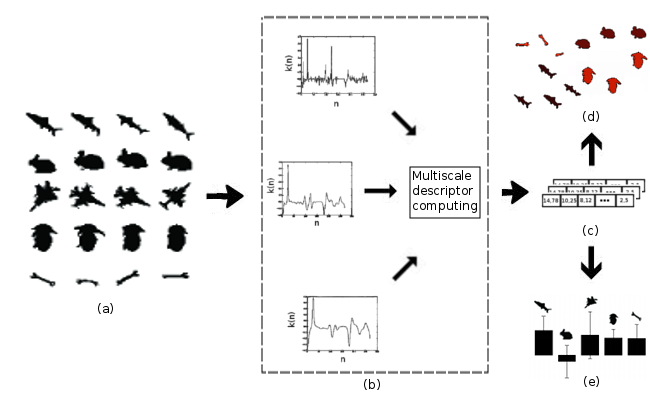
\includegraphics[width=\textwidth]{metodo_v4.png}
\end{figure}

O primeiro passo consiste em realizar a extração de características num conjunto de formas binárias rotuladas (Figura \ref{fig:metodo_4}a e Figura \ref{fig:metodo_4}b) com o método de descrição sob análise. Como resultado temos um conjunto de descritores, ou vetores de características, das referidas formas (Figura \ref{fig:metodo_4}c). 

A avaliação de qualidade dos descritores se dá qualitativamente e quantitativamente. Na avaliação qualitativa (Figura \ref{fig:metodo_4}d) utilizamos a rede auto-organizável de Kohonen para obtenção da matriz de distâncias unificada, ou matriz-U. Essa última é empregada como ferramenta de visualização dos dados, o que possibilita identificar como o método de descrição sob avaliação agrupa as formas. 

Na avaliação quantitativa (Figura \ref{fig:metodo_4}e) utilizamos os rótulos e os vetores de características das formas para calculamos a medida de avaliação de agrupamentos \emph{Silhouette} \cite{Rousseeuw:1987}. Valores médios dessa medida, por classe de formas, indica a habilidade dos descritores em discriminar formas que pertençam a classes distintas e de agrupar formas que pertençam a uma mesma classe.
\end{comment}

Com o método de otimização proposto realizamos experimentos de classificação e recuperação de formas pelo conteúdo, para dois descritores, com a base de folhas de plantas Flavia \cite{4458016},  que possui $1907$ imagens de folhas de $32$ espécies. A Figura \ref{fig:bases} ilustra imagens das folhas desta base. Cada exemplar ilustrado foi segmentado e colorido de acordo com a espécie ao qual pertence. Essa base de folhas é amplamente utilizada na validação de trabalhos de reconhecimento automático de espécies de plantas. 

\begin{figure}[!htb]
\centering
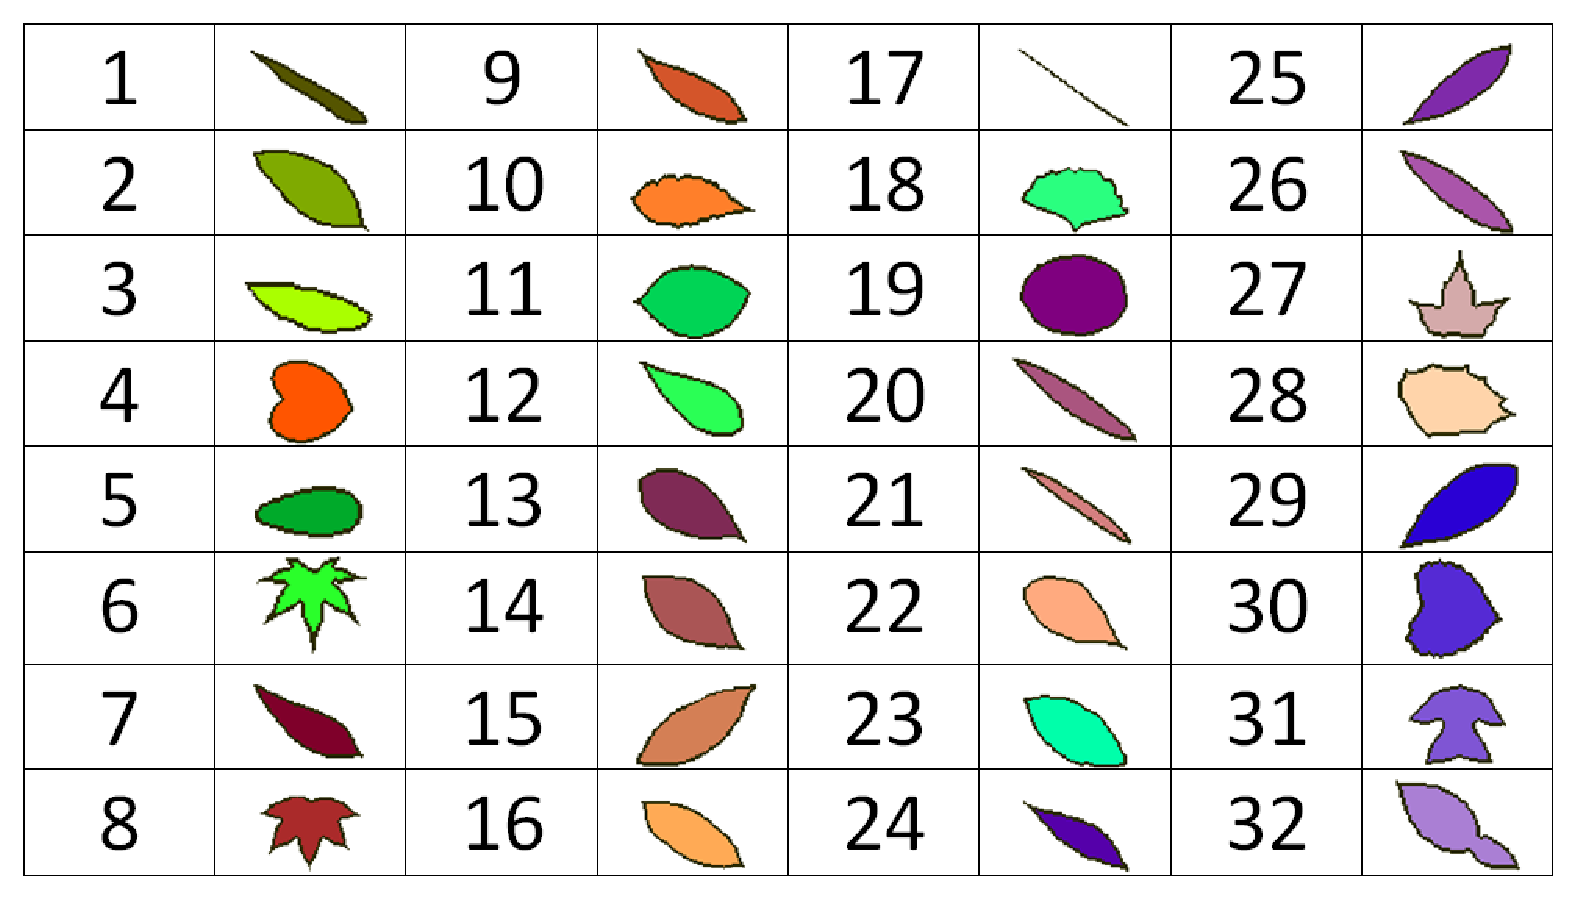
\includegraphics[width=0.5\textwidth]{fig5.eps}
\caption{\label{fig:bases}Samples of Flavia leaf data set.}
\end{figure}


% !TeX root = ../main.tex

\chapter{Resultados e Discussões \label{chap:resultados}}


Com o método de otimização proposto realizamos experimentos de classificação e recuperação de formas pelo conteúdo, para dois descritores, com a base de folhas de plantas Flavia \cite{4458016},  que possui $1907$ imagens de folhas de $32$ espécies. A Figura \ref{fig:bases} ilustra imagens das folhas desta base. Cada exemplar ilustrado foi segmentado e colorido de acordo com a espécie ao qual pertence. Essa base de folhas é amplamente utilizada na validação de trabalhos de reconhecimento automático de espécies de plantas. 

\begin{figure}[!htb]
\caption{\label{fig:bases}Amostras de formas de folhas da base de imagens Flavia.}

\centering
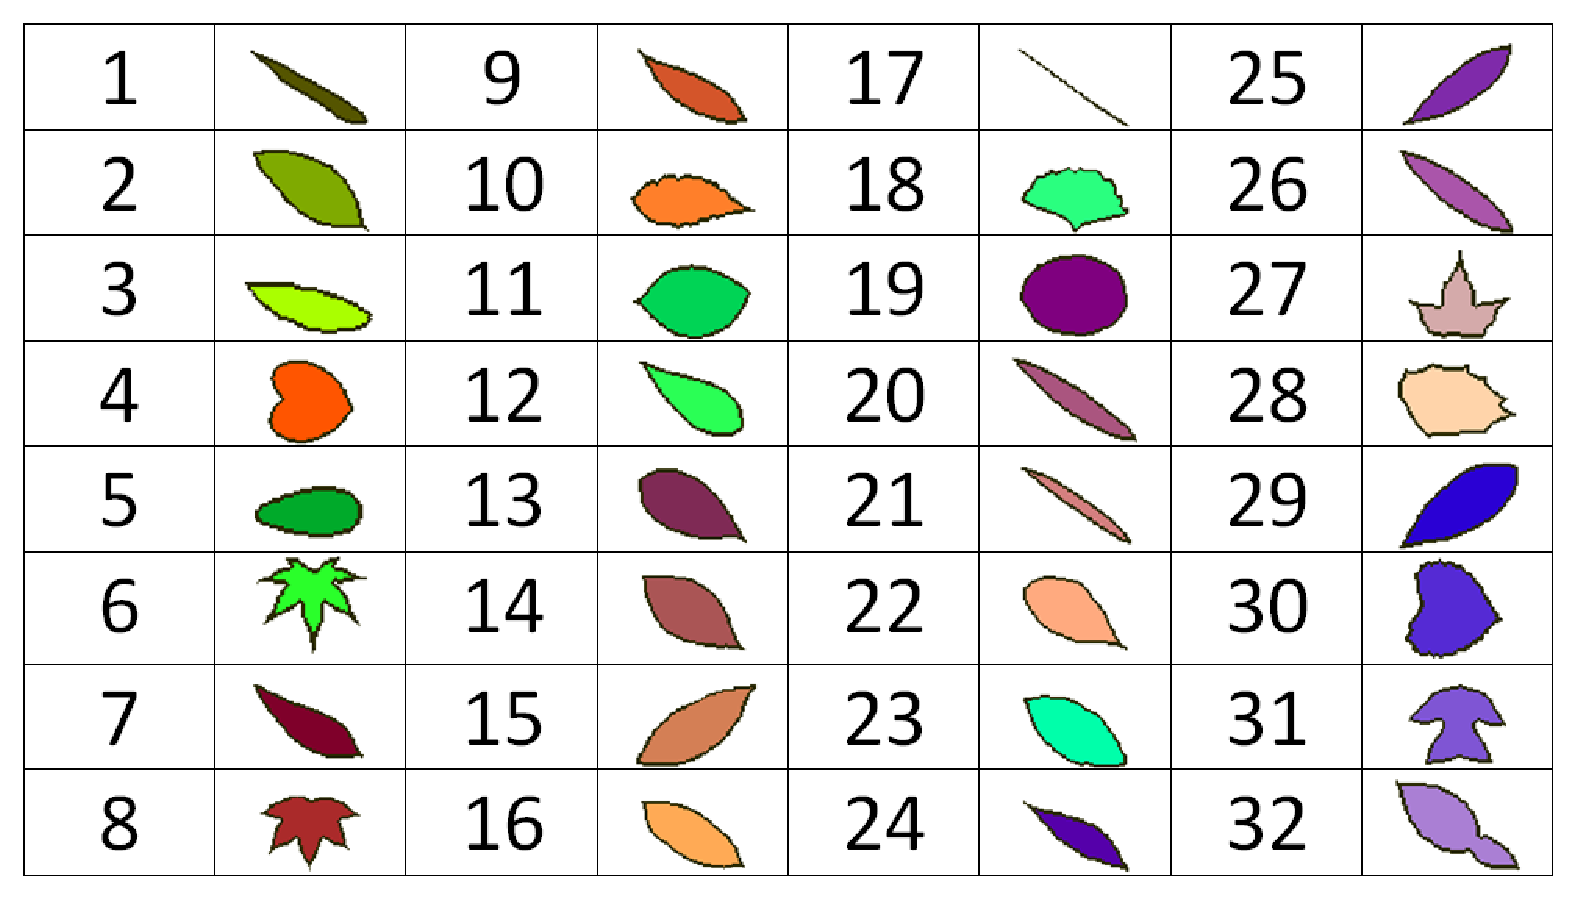
\includegraphics[width=0.5\textwidth]{fig5.eps}
\end{figure}





{\color{blue}

\section{\emph{Classificação de formas e sua relação com  a função objetivo}}
Foram realizados experimentos para comparação dos algoritmos de otimização sob aspecto de convergência. A Figura \ref{fig:converge} ilustra a convergência de cada um dos três algoritmos de otimização para $30$ repetições realizadas em um subconjunto da base de formas de folhas. Os resultados obtidos indicam que a otimização \emph{PSO} requereu um pequeno número de interações para convergir a uma solução ótima quando comparado aos algoritmos \emph{SA} e \emph{DE}. Uma vez que a convergência está relacionada com o número de interações necessárias para se atingir uma solução ótima, poucas interações implicam em uma em exploração deficiente do espaço de busca, ou seja, em convergência prematura \citeonline{Andries:2007}. Nesse caso, o método de otimização apresenta tendência de ficar preso a mínimos locais, encontrando assim soluções sub-ótimas para o problema. Por outro lado, a convergência mais lenta permite ao algoritmo explorar melhor o espaço de busca, aumentando portanto a chance deste convergira um mínimo global, ou seja, uma solução ótima \citeonline{Andries:2007}.
 
Neste contexto, observa-se na Figura \ref{fig:converge}c que o \emph{PSO} encontrou soluções sub-ótimas com maior frequência, alcançando valores médios da função MAD  igual a $0,805 \pm 0,006$.  Já os algoritmos \emph{SA} e \emph{DE} alcançaram os menores valores médios de MAD : $0,795 \pm 0,006$ e $0,798 \pm 0,004$, respectivamente. 

Logo, esses resultados demonstram que os algoritmos \emph{SA} e \emph{DE} foram mais eficazes que o \emph{PSO} em encontrar soluções ótimas. No entanto, o custo para alcançar tais soluções torna-se maior. A Seção \ref{sec:comp_cost} trata em mais detalhes as questões relativas ao custo computacional dos algoritmos de otimização utilizados.

\begin{figure}[!htb]
\caption{\label{fig:converge}{\color{red} SUGIRO COLOCAR NA METODOLOGIA PARA ESCOLHER LÁ O SA} Convergência dos métodos de otimização para o problema de descrição de folhas de plantas: (a) SA, (b) DE, (c) PSO. As curvas em vermelho destacam o valor médio da função MAD para $30$ realizações de cada método (curvas em preto). }
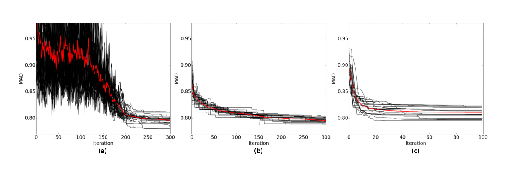
\includegraphics[width = \textwidth]{fig6.eps}
\end{figure}

Para a próxima análise assume-se a hipótese de que as escalas otimizadas e o valor ótimo de MAD, que estão inter-relacionadas, implicam em melhorias na taxa de classificação correta das espécies. Na Tabela \ref{tab:leaves_supervised_results} estão apresentados diversos valores de MAD e os correspondentes resultados em experimentos de classificação para diferentes classificadores. Observa-se que os melhores resultados de classificação correspondem aos menores valores de MAD obtidos através da otimização. Os resultados de classificação para o descritor \emph{NMBE}, com as escalas ajustadas conforme sugerido por \citeonline{Costa:1997} ($\operatorname{NMBE_{orig}}$), resultou em um desempenho intermediário quando comparado aos resultados para escalas otimizadas e escolhidas arbitrariamente. Logo, o descritor \emph{NMBE} otimizado ($\operatorname{NMBE_{opt}}$) melhorou o desempenho de todos os classificadores avaliados, uma vez que este alcançou as maiores taxas de Precisão e Revocação rates para os menores valores de MAD, o que confirma a hipótese inicial.

Apesar do descritor \emph{NMBE} ter sido originalmente projetado para descrição de neurônios, nosso trabalho aplicou-o com sucesso em caracterização de folhas de plantas, uma vez que a otimização o adequou ao problema em questão.
Embora os diferentes algoritmos de otimização tenham atingido valores de MAD diferentes, e portanto conjuntos de escalas otimizadas distintas, os resultados dos experimentos de classificação mostraram corroboraram a conclusão anterior, pois tais conjuntos de escalas foram adequadas para gerar descritores capazes de capturar informações de detalhes que diferenciem apropriadamente as formas das folhas. Logo, os algoritmos de otimização trazem vantagens à representação multiescala com impacto significativo na caracterização das folhas. 

\begin{table}[]
\begin{minipage}{\textwidth}
\renewcommand\footnoterule{}
\caption{Valores de MAD e resultados de classificação das espécies vegetais da base de imagens Flavia para diferentes estratégias de escolha das escalas do descritor \emph{NMBE}. }
\label{tab:leaves_supervised_results}
\resizebox{\textwidth}{!}{ 
\begin{tabular}{cccccccccc}
\toprule[1.5pt]
 & \multicolumn{8}{c}{Classifier} \\ \cmidrule(lr){2-9} 
 & \multicolumn{2}{c}{NB}  & \multicolumn{2}{c}{Knn (n = 5)}  & \multicolumn{2}{c}{LDA}  & \multicolumn{2}{c}{QDA} \\
\cmidrule(lr){2-3}  \cmidrule(lr){4-5} \cmidrule(lr){6-7}  \cmidrule(lr){8-9}
MAD & Precision & Recall & Precision & Recall & Precision & Recall & Precision & Recall \\ \midrule
$0,762$\footnote{Using SA}        & ${0,91 \pm 0,02}$   & ${0,89 \pm 0,02}$         & ${0,93 \pm 0,02}$          & ${0,92 \pm 0,02}$         & ${0,87  \pm 0,02}$          & ${0,85\pm 0,02}$         & ${0,95  \pm 0,01}$          & ${0,94  \pm 0,01}$         \\
$0,783$\footnote{Using DE}        & $0,88 \pm 0,02$          & $0,87\pm0,02$         & $0,90\pm0,02$          & $0,88\pm0,02$         & $0,85\pm0,02$          & $0,83\pm0,03$         & $0,91\pm0,02$          & $0,90\pm0,02$         \\
$0,829$\footnote{Using PSO}        & $0,86\pm0,03$          & $0,85\pm0,03$         & $0,89\pm0,03$          & $0,88\pm0,03$         & $0,84\pm0,03$         & $0,82\pm0,03$         & $0,91\pm0,02$          & $0,89\pm0,02$         \\
{$0,867$\footnote{Using scales proposed by \citeonline{Cesar:1996}}}          & $0,85\pm0,02$          & $0,84\pm0,02$         & $0,89\pm0,02$          & $0,88\pm0,02$         & $0,82\pm0,03$          & $0,81\pm0,03$         & $0,89\pm0,02$          & $0,88\pm0,02$         \\
{$0,969$\footnote{\label{note1}Random selection}}          & $0,81\pm0,03$          & $0,79\pm0,03$         & $0,87\pm0,02$          & $0,85\pm0,02$         & $0,77\pm0,03$          & $0,77\pm0,03$         & $0,87\pm0,03$          & $0,85\pm0,03$         \\
{$1,04$\footref{note1}}          & $0,69\pm0,03$          & $0,68\pm0,03$         & $0,83\pm0,03$          & $0,82\pm0,03$         & $0,74\pm0,03$          & $0,73\pm0,03$         & $0,81\pm0,03$          & $0,79\pm0,03$         \\
\bottomrule[1.5pt]
\end{tabular}}
\end{minipage}
\end{table}
  
Por último, observa-se que os classificadores que utilizaram descritores gerados a partir de escalas selecionadas arbitrariamente não tiveram desempenho satisfatório, pois alcançaram os menores valores de Precisão e Revocação e os maiores valores da função MAD. Portanto, escalas aleatórias levam a uma representação multiescala menos sensível a variações de características das folhas, consequentemente, mais erros de classificação. 


\section{\emph{Análise exploratória visual de agrupamentos}}
A análise exploratória visual dos agrupamentos  produzidos pela descrição NMBE das folhas indica que a descrição otimizada melhora a organização dos agrupamentos, o que reforça que a função objetivo MAD é adequada para guiar o processo de otimização desse descritor. A Figura \ref{fig:MatrizU_leaves_256}  ilustra a visualização da descrição das folhas através  das matrizes-U. Em cada posição da matriz, os valores numéricos da foram substituídos pela imagem das folhas correspondentes, estando as cores das folhas em correspondência com o rótulo das classes exibidas na Figura \ref {fig:bases}. Nessas matrizes-U estão representadas as $1907$ formas de folhas da base Flávia, sendo cada folha representada por sua descrição multiescala.

A Figura \ref{fig:MatrizU_leaves_256}a mostra a matriz-U obtida para as formas de folhas representadas pelo descritor NMBE otimizado e a Figura \ref{fig:MatrizU_leaves_256}b, pelo descritor NMBE não otimizado. Os gráficos representativos da medida \emph{silhouette} nas respectivas figuras demonstram que as classes das folhas caracterizadas e, portanto, agrupadas adequadamente são as que apresentam valores de \emph{silhouette} média positivos. Por outro lado, as classes de folhas que o descritor não foi capaz de caracterizar e agrupar adequadamente são as que apresentaram valores negativos de \emph{silhouette} média. Comparando ambas as figuras, observa-se que na Figura \ref{fig:MatrizU_leaves_256}a há expressiva redução dos valores negativos de \emph{silhouette} média para a caracterização das folhas com o descritor $\operatorname{NMBE_{opt}}$. 

\begin{figure}[t]
\caption{\label{fig:MatrizU_leaves_256} Matrizes-U e a \emph{silhouette} média para as descrições das folhas da base Flavia com o descritor NMBE (a) optimizado e (b) não otimizado.}
\centering
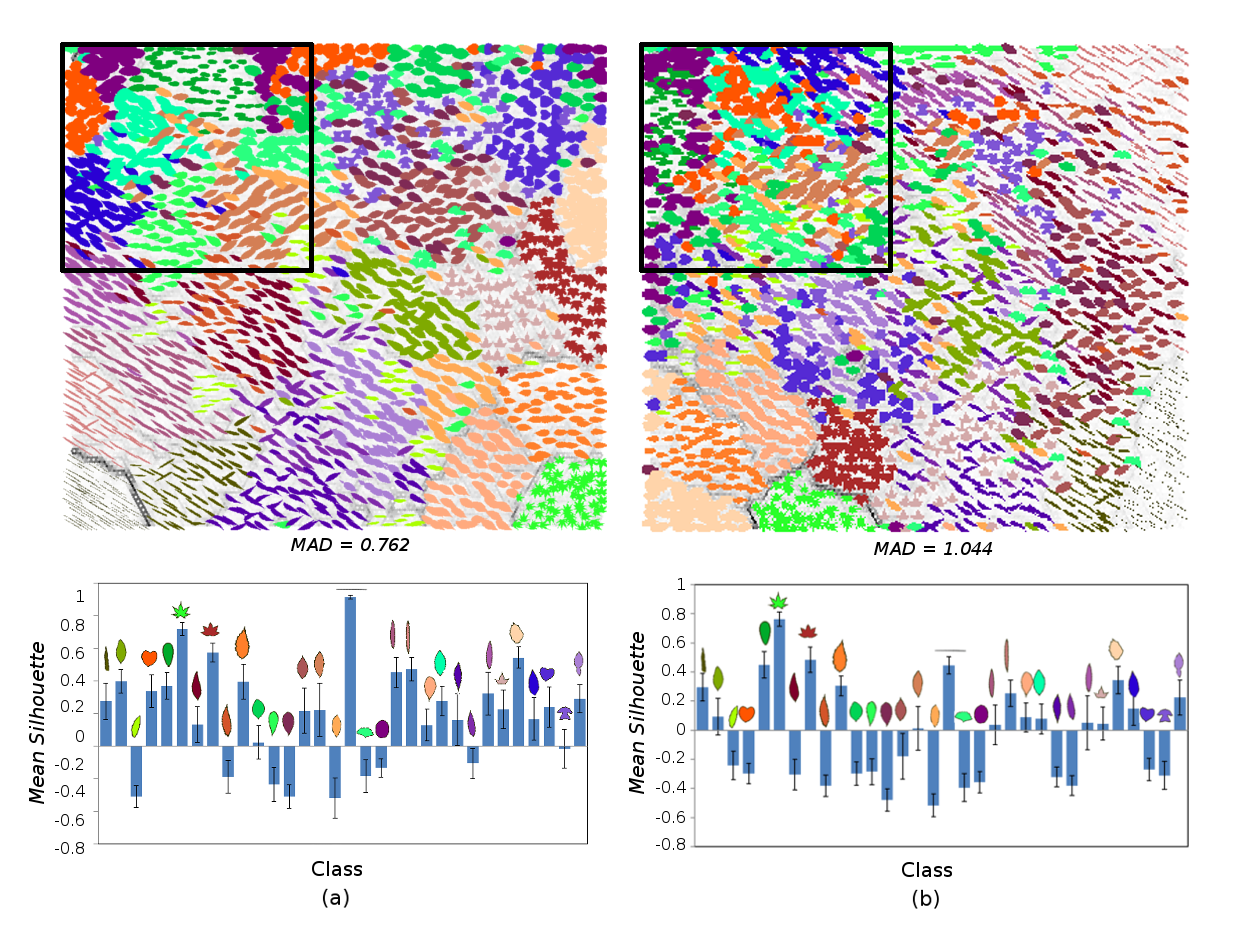
\includegraphics[width=\textwidth]{fig7.eps}
\end{figure}
}
{\color{red}
The black square in Figure \ref{fig:MatrizU_leaves_256}a highlights  the performance of the optimized descriptor. It also shows how well the optimized descriptor mapped leaf shapes into groups according to their respective classes.  Moreover, the optimized descriptor has remarkably improved  the mean \emph{silhouette} per class for almost all leaf classes. In contrast, the region inside the black square in Figure \ref{fig:MatrizU_leaves_256}b indicates that the non-optimized descriptor was unable to satisfactorily map leaf shapes in their corresponding classes.
These results  indicated that the optimized descriptor has improved the cluster arrangement of leaves due to the intrinsic shape variations within the set of optimized scales that can not be properly embodied in the studied traditional parameter selection methods.

Figures \ref{fig:MatrizU_leaves_II}a, \ref{fig:MatrizU_leaves_II}b and \ref{fig:MatrizU_leaves_II}c display the U-matrices and the corresponding MAD values for experiments on Flavia leaf data set with SA, DE and PSO, respectively. An interesting aspect to examine in these results regards the convergence of the optimization algorithms to different solutions (MAD). These solutions resulted in different cluster arrangements and therefore different relations among the neighborhood structure of clusters. For instance, the overall dispersion  of the elements in Figure \ref{fig:MatrizU_leaves_II}a and Figure \ref{fig:MatrizU_leaves_II}b tend to be very similar since  the corresponding MAD values are close to each other. At the same time, the result that corresponds to the highest MAD value ($0.829$) exhibits a relatively high dispersion within clusters, particularly at the center of the U-matrix (Figure \ref{fig:MatrizU_leaves_II}c), which reinforces the hypothesis that  PSO converged to a local minimum. These findings point to the important conclusion that the lower the MAD value, the better the cluster arrangement and hence the cluster quality. Therefore, we state that the cluster quality and MAD value are negatively correlated. Our analysis also considers that there are other solutions than the minimum, in the search space, which may be suitable to the problem under study. 

\begin{figure}[h!]
 \caption{\label{fig:MatrizU_leaves_II}Matrices-U e valores MAD obtidos para a base de imagens Flavia por uso da NMBE otimizada pelos algoritmos (a) SA, (b) DE, (c) PSO.}
\centering
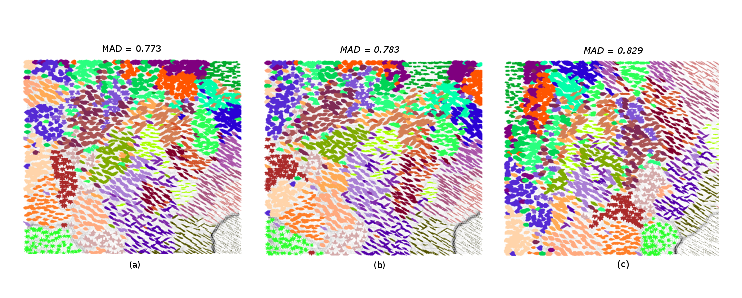
\includegraphics[width=\textwidth,trim = 0mm 0mm 0mm 4.5mm,clip]{fig8.eps}
\end{figure}

Figure \ref{MDS:Leaves} illustrates the MDS projections for three different MAD values. Figure \ref{MDS:Leaves}a corresponds to the cluster arrangement after the convergence of the SA algorithm, i.e. after reaching the minimum MAD value. These projections confirmed that the minimization of the objective function provided leaf cluster arrangements with lower average within-class distances and higher inter-class distances, and thus  more compact and separated clusters. The visual analysis of the three detail images in Figure \ref{MDS:Leaves}a discloses that the MDS projection of the optimized NMBE descriptor increased inter-class distances, whereas it reduced the within-class distances when compared to Figure \ref{MDS:Leaves}b and \ref{MDS:Leaves}c. Moreover, the $R^2$ coefficient values close to 1 imply that the low-dimensional representation preserved the mean distance in the original high-dimensional data space.

\begin{figure}[h!]
 \caption{\label{MDS:Leaves} Projeções MDS dos descritores NMBE para formas da base de folhas Flavia. (a) Descritor NMBE otimizado pelo algoritmo SA com valor de função $MAD = 0,762$ (b) Descritor NMBE não otimizado com valor de função $MAD =0,969$ and (c) Descritor NMBE não otimizado com valor de função $MAD = 1,044$.}

\centering
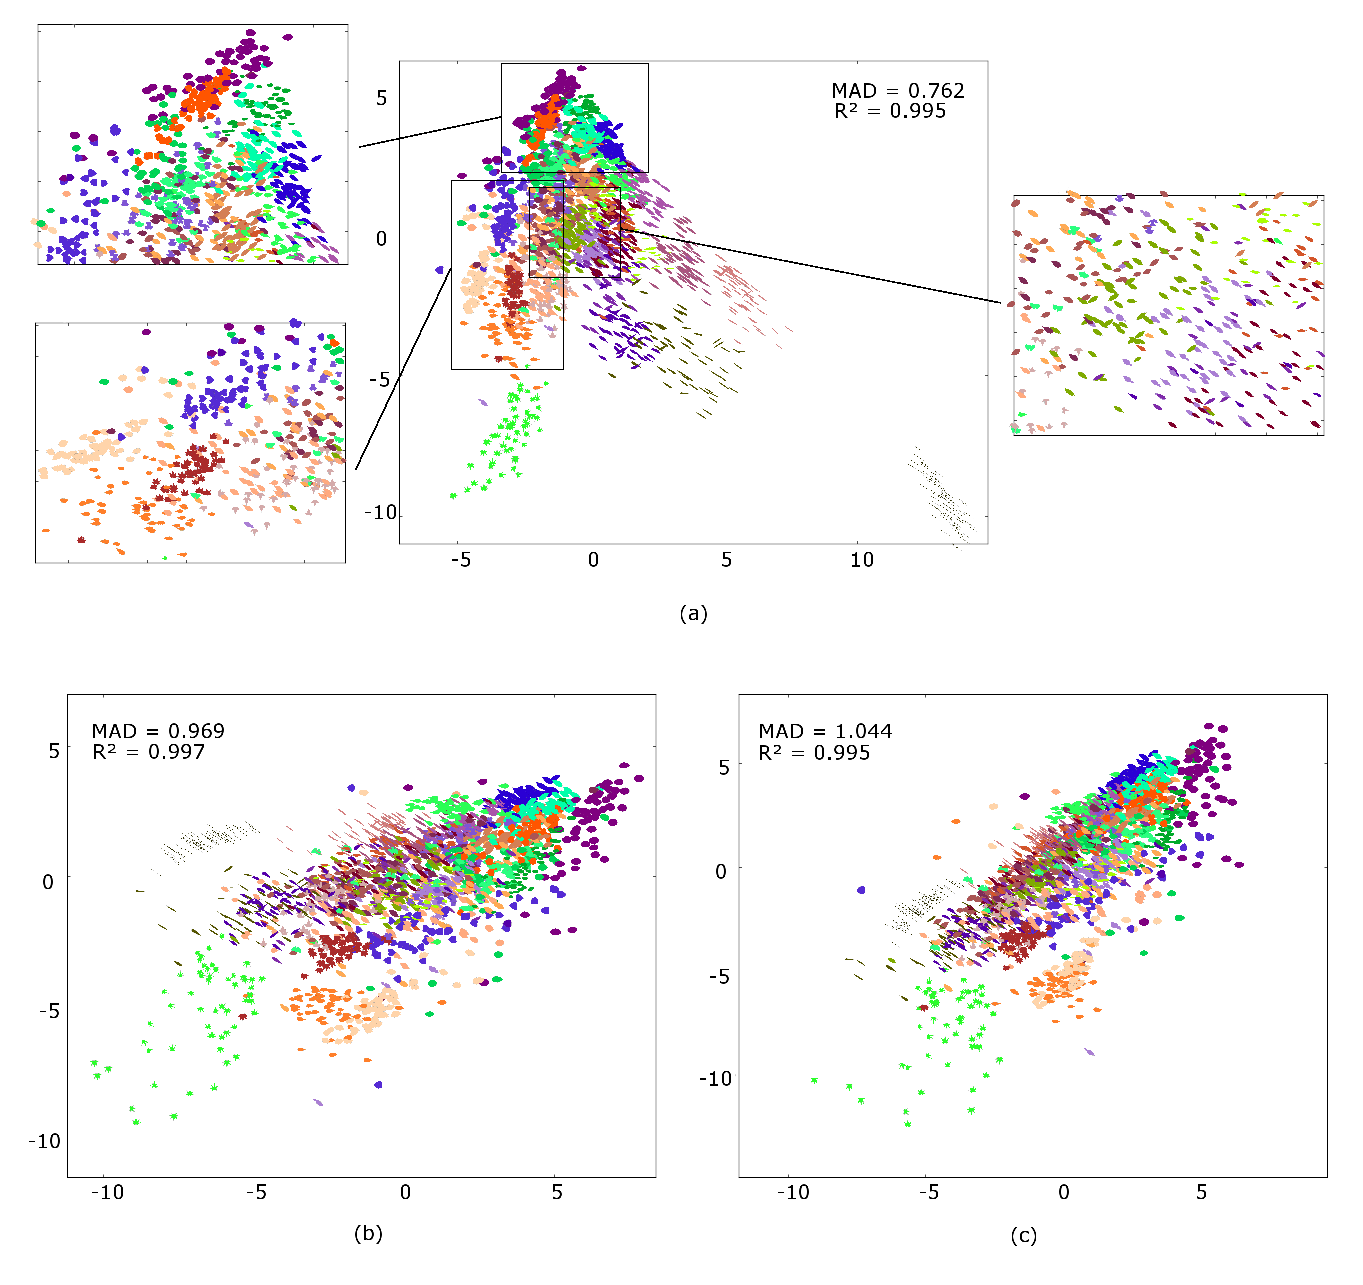
\includegraphics[width=\textwidth]{fig9.eps}
\end{figure}
\section{\emph{Recuperação de imagens baseada em conteúdo - CBIR}}
For the sake of comparison, we have optimized the parameters of another shape descriptor namely inner distance shape context (IDSC) \citeonline{Ling:2007:SCU:1191552.1191806}.
This descriptor is mainly applied to shape retrieval, which involves unsupervised shape classification tasks.  Moreover, IDSC employs dynamic programming (DP), such as Dynamic Time Warping (DTW) \citeonline{PalazonGonzalez2012978}, to improve shape matching accuracy. In this paper, we have replaced the $L_2$ norm by DTW to compute the \emph{silhouette} measure and the cost function defined in equation \ref{eq:mad}.  
Figure \ref{figfig1Optmization-IDSC} exhibits the comparison of shape retrieval experiments which were performed on the public Flavia leaf data set and with both non-optimized NMBE and IDSC and their optimized counterparts ($\operatorname{NMBE_{opt}}$, $\operatorname{IDSC_{opt}}$).
The performance evaluation methodology has adapted the Bulls-eye measure, where the result is the overall number of shapes correctly  retrieved, in each rank position, for each shape in data set taken as a query.  Let $N_c$ be the number of shapes which belong to the class $c$. Here, the number of retrieved shapes ($N_r$) was adjusted to $N_r = 2\displaystyle \min_{c = 1,2,\dots 32}{N_c}$. Figure \ref{figfig1Optmization-IDSC} also demonstrates that the optimization methodology was decisive for both descriptors to achieve better retrieval rates. 
Figure \ref{fig1Ooptimization_graph}  shows that after tuning IDSC parameters for the Flavia leaf data set with the optimization methodology the retrieval rate has remarkably increased. Therefore, $\operatorname{IDSC_{opt}}$  outperformed the optimized NMBE ($\operatorname{NMBE_{opt}}$) and non-optimized NMBE. In this sense, the optimized parameters of $\operatorname{IDSC_{opt}}$ may have incorporated subtle details of leaf shapes. On the other hand, we have observed that the non-optimized IDSC underperformed the non-optimized NMBE. 
In order to provide a non-optimized counterpart of IDSC, we have followed the parameter setting introduced in \citeonline{wang2015march}.
Figure \ref{subfig:upper-right} and \ref{subfig:lower-right} exemplify samples of  plant leaves which were retrieved according to the rank of the similarity to the two queries. These results have demonstrated that the non-optimized descriptors in Figure \ref{subfig:upper-right} and \ref{subfig:lower-right} were unable to retrieve all samples for the two queries, whereas the  optimized descriptors retrieved all of them, correctly.

\begin{figure}[]
\caption{Experimentos realizados com formas da base de imagens de folhas Flavia (a) taxa de recuperação  obtida com os descritores NMBE e IDSC originais e suas versões otimizadas, (b) e (c)recuperação de duas amostras de folhas utilizando os descritores NMBE e IDSC otimizados e não otimizados, respectivamente.  respectively.\label{fig1Ooptimization_graph}}
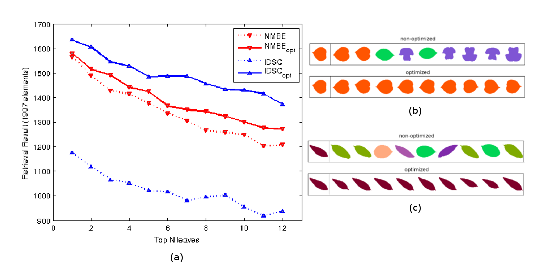
\includegraphics[width=\textwidth]{fig10.eps}
\end{figure}

\begin{comment}
\begin{figure}[t!]
\begin{subfigure}{0.55\textwidth}
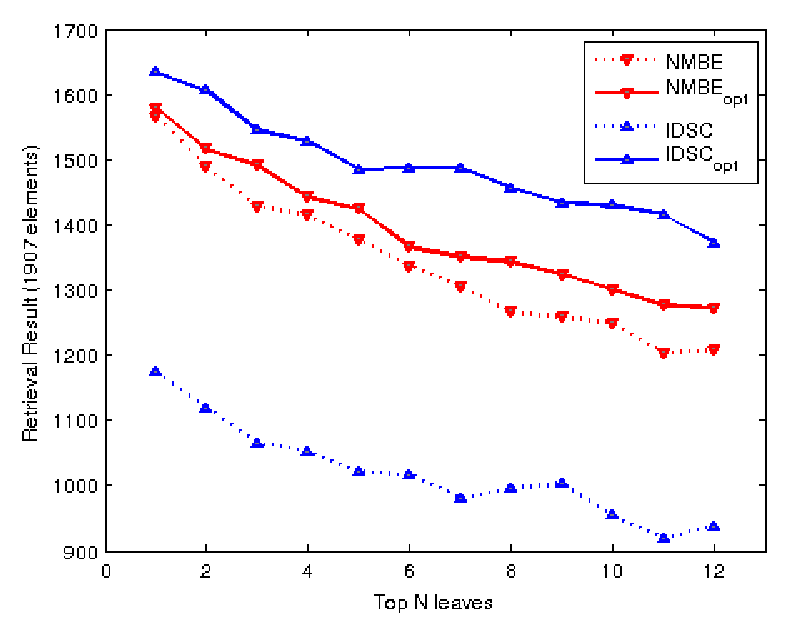
\includegraphics[width=\textwidth]{fig10a.eps}
\caption{Retrieval rates. \label{fig1Ooptimization_graph}}
\end{subfigure}
\hspace*{\fill}
\begin{minipage}{0.45\textwidth}
\begin{subfigure}{\textwidth}
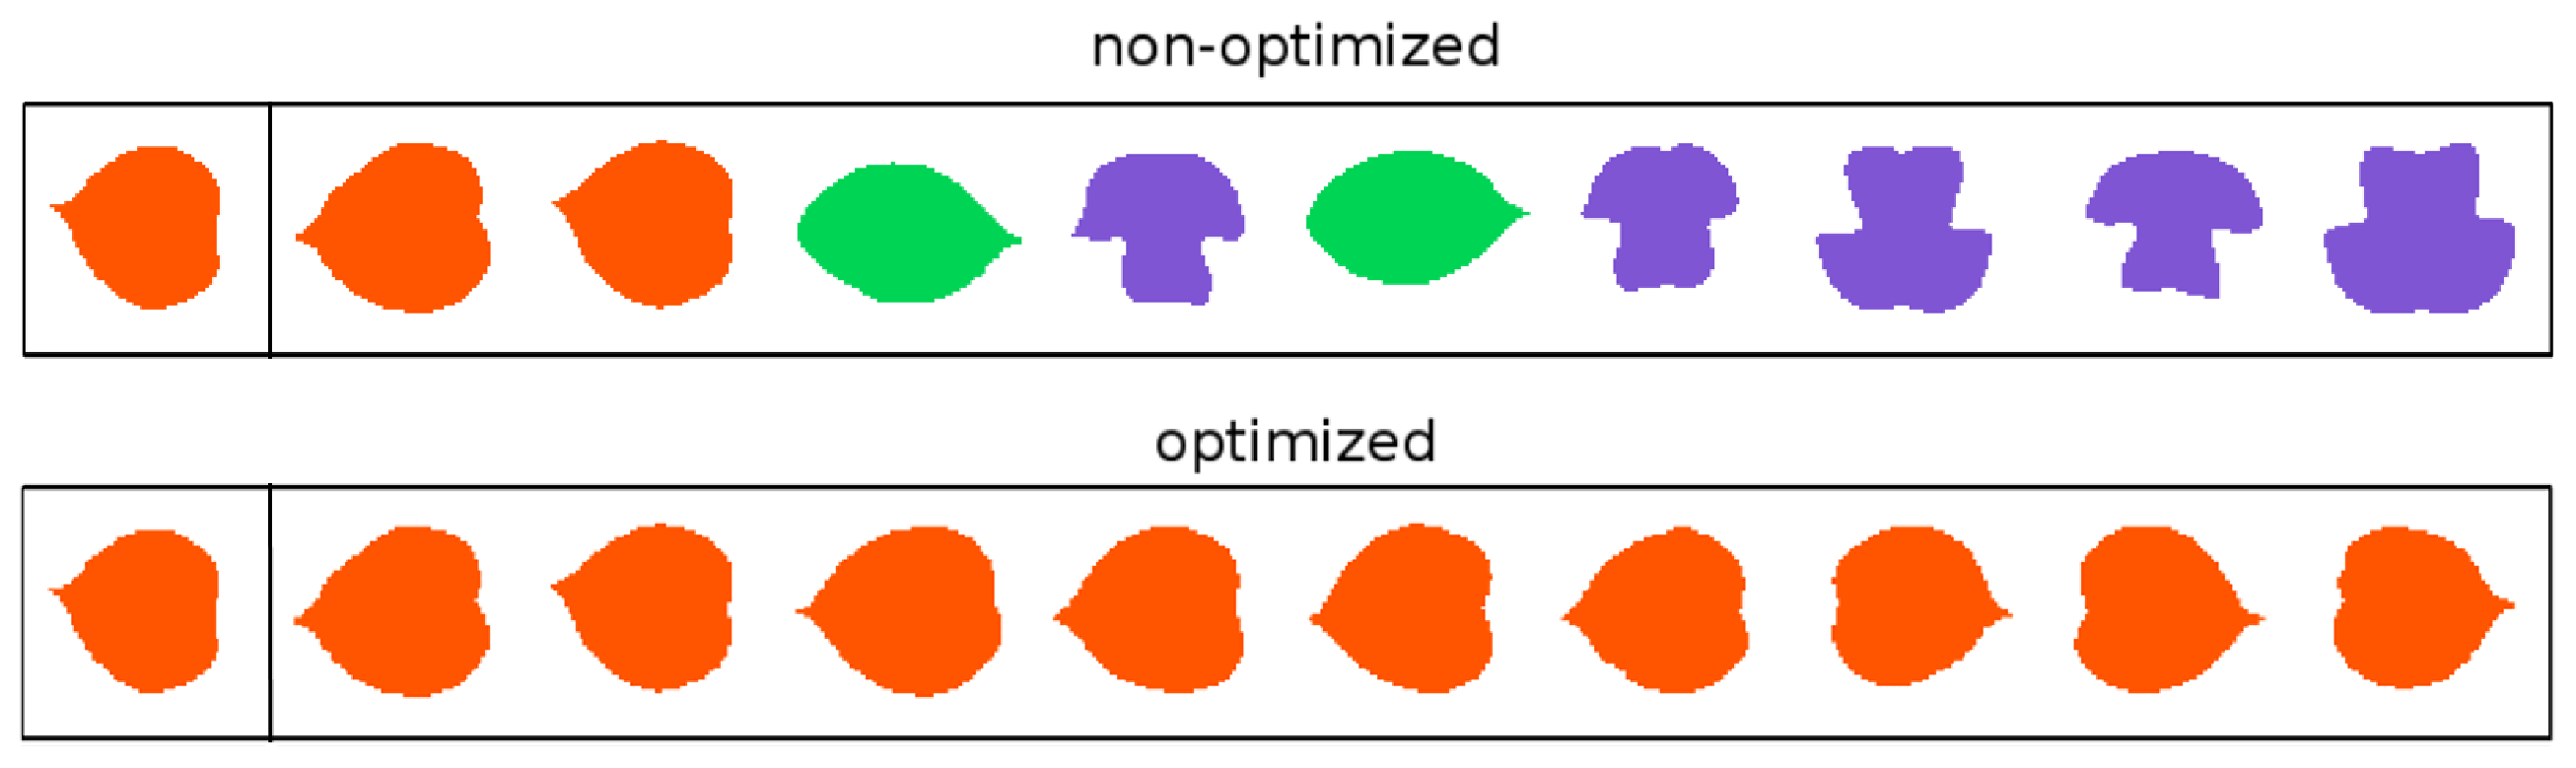
\includegraphics[width=\textwidth]{fig10b.eps}
\caption{Retrieval results with NMBE.} \label{subfig:upper-right}

\end{subfigure}

\vspace*{0.60cm}
\begin{subfigure}{\textwidth}
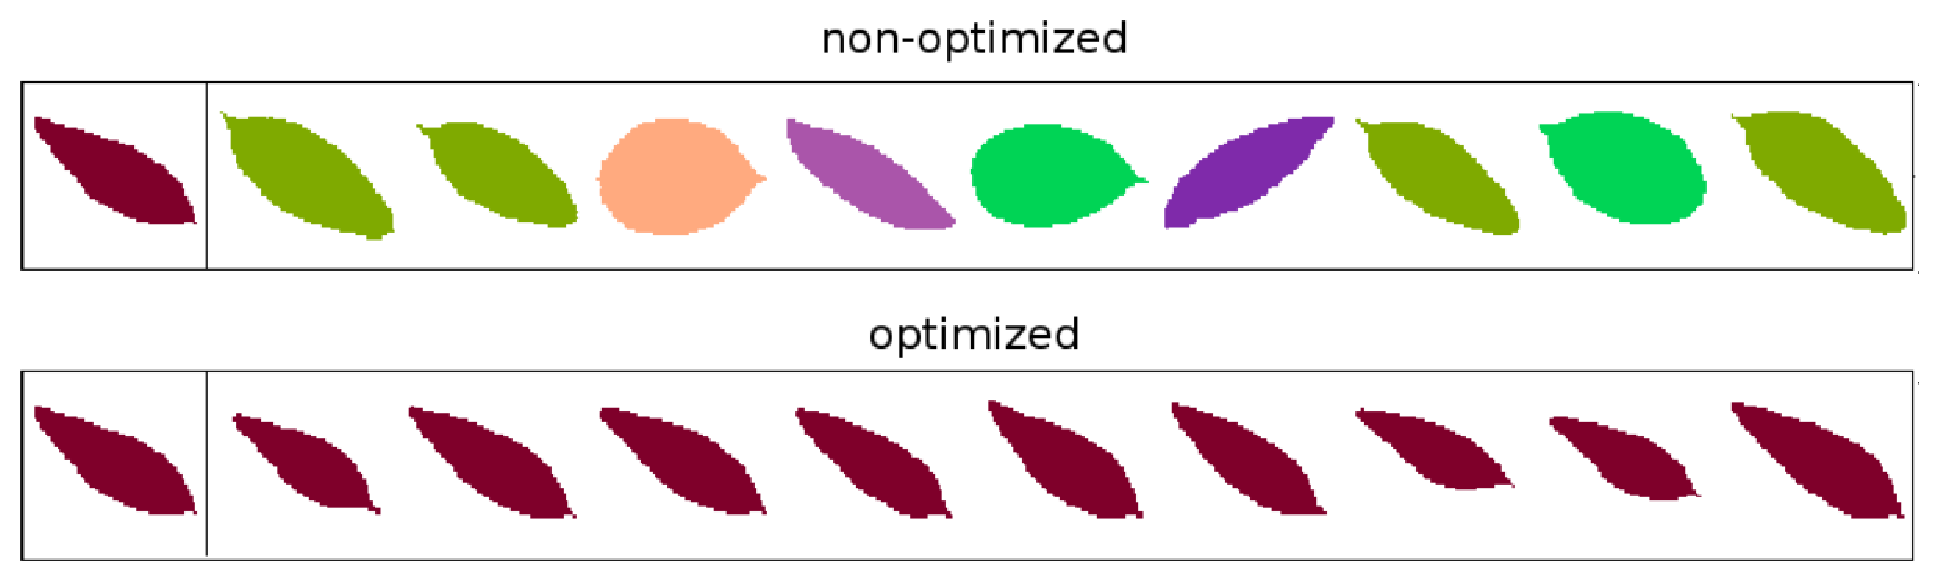
\includegraphics[width=\textwidth]{fig10c.eps}
\caption{Retrieval results with IDSC.\label{subfig:lower-right}}
\end{subfigure}
\end{minipage}

\caption{\label{figfig1Optmization-IDSC} Experiments conducted on Flavia leaf data set (a) retrieval rate by using both NMBE and IDSC and their optimized counterparts, (b) and (c) two leaf shape retrieval examples by using the non-optimized and optimized NMBE and IDSC descriptors, respectively.} 
\end{figure}
\end{comment}

 Table \ref{table_bull_eyes_leaves} presents the performance evaluation of NMBE, whose scales were computed using the scheme introduced by \citeonline{Cesar:1996}, IDSC and their optimized counterparts.  The retrieval rates show that both optimized descriptors outperformed their non-optimized counterparts on Flavia data set. The remarkable improvement on the Bulls-eye rates reinforces our assumption that the optimization methodology is suitable for leaf shape retrieval and analysis.

\begin{table}[h!]
\centering
\caption{Taxa Bulls-eye para a base de imagens Flavia.}
\label{table_bull_eyes_leaves}
  \begin{tabular}{cccccccc}
  \toprule[1.5pt]
 $\operatorname{NMBE}$ & $\operatorname{NMBE_{opt}}$ & IDSC    & $\operatorname{IDSC_{opt}}$\\ \midrule
     63.86 \%  & 71.16 \%  & 53.38\%    & 77.50\%       \\
  \bottomrule[1.5pt]
  \end{tabular}
\end{table}

Thus, we can infer that the optimized descriptors are more likely to succeed in shape retrieval experiments because the optimized sets of parameters probably embody intrinsic and subtle information about leaf shapes. We can also assume that these optimized descriptors may reliably characterize and also discriminate shape differences within and among leaf classes. 

\subsection{Computational cost \label{sec:comp_cost}}

Table \ref{tbl:complexity} shows the computational complexity results of the three optimization algorithms. SA and PSO present similar complexity results which rely on the number of iterations to converge ($N_{iter}$), population size ($N_{pop}$) and $P$ parameter. On the other hand,  DE  demands a higher complexity which relies on the dimension of the optimization problem ($D$), population size ($N_{pop}$) and number of iterations to converge ($N_{iter}$).

\begin{table}[h!]
\centering
\caption{Complexidade computacional dos métodos de otimização.}
\label{tbl:complexity}
  \begin{tabular}{ll}
  \toprule[1.5pt]
 Método & Complexidade\\
 \midrule
   SA  & $O(P.N_{iter}.\log{N_{iter}})$    \\
   DE  & $O(N_{pop}.N_{iter}.D)$   \\
   PSO&  $O(N_{pop}.N_{iter}.\log{N_{iter}})$\\
  \bottomrule[1.5pt]
  \end{tabular}
\end{table}

For the sake of comparison, we assumed that the computational cost is the number of times that the objective function is demanded throughout the optimization process. Its calculation takes into account the parameter setting of each method, presented in Section \ref{subsec:opmet}, and the corresponding computational complexity.  The computational cost to address the optimization of the multiscale descriptor for SA, DE and PSO yielded $7,4314$, $19,500$ and $1,107$, respectively. 

It is worth noting that there is a trade-off between the computational cost and the quality of the optimal solution found. Although the reduction of the number of shape samples, image resolution and the $N_{pop}$ variable can lessen the computational cost, it may degrade the optimization result. Moreover, parallelism may contribute to reduce the computational cost without degrading the optimization result.  However, it adds an extra computational complexity to the optimization algorithms.
}


%\section{Visualização dos dados}

%\subsection{\emph{DFM}}


Com base na metodologia exposta apresentamos neste capítulo os resultados experimentais obtidos na análise dos descritores dimensão fractal multiescala, energia de dobramento multiescala Uma avaliação comparativa dos resultados obtidos com os descritores \emph{NMBE} e \emph{DFM} é apresentada na seção a seguir.

\begin{figure}
 \caption{\label{fig:dfm99} (a) Matriz-U para as formas da base Kimia99 representadas com o descritor dimensão fractal multiescala. (b) \textit{Silhouette} média por classe obtida a partir do referido descritor.}
  \centering
  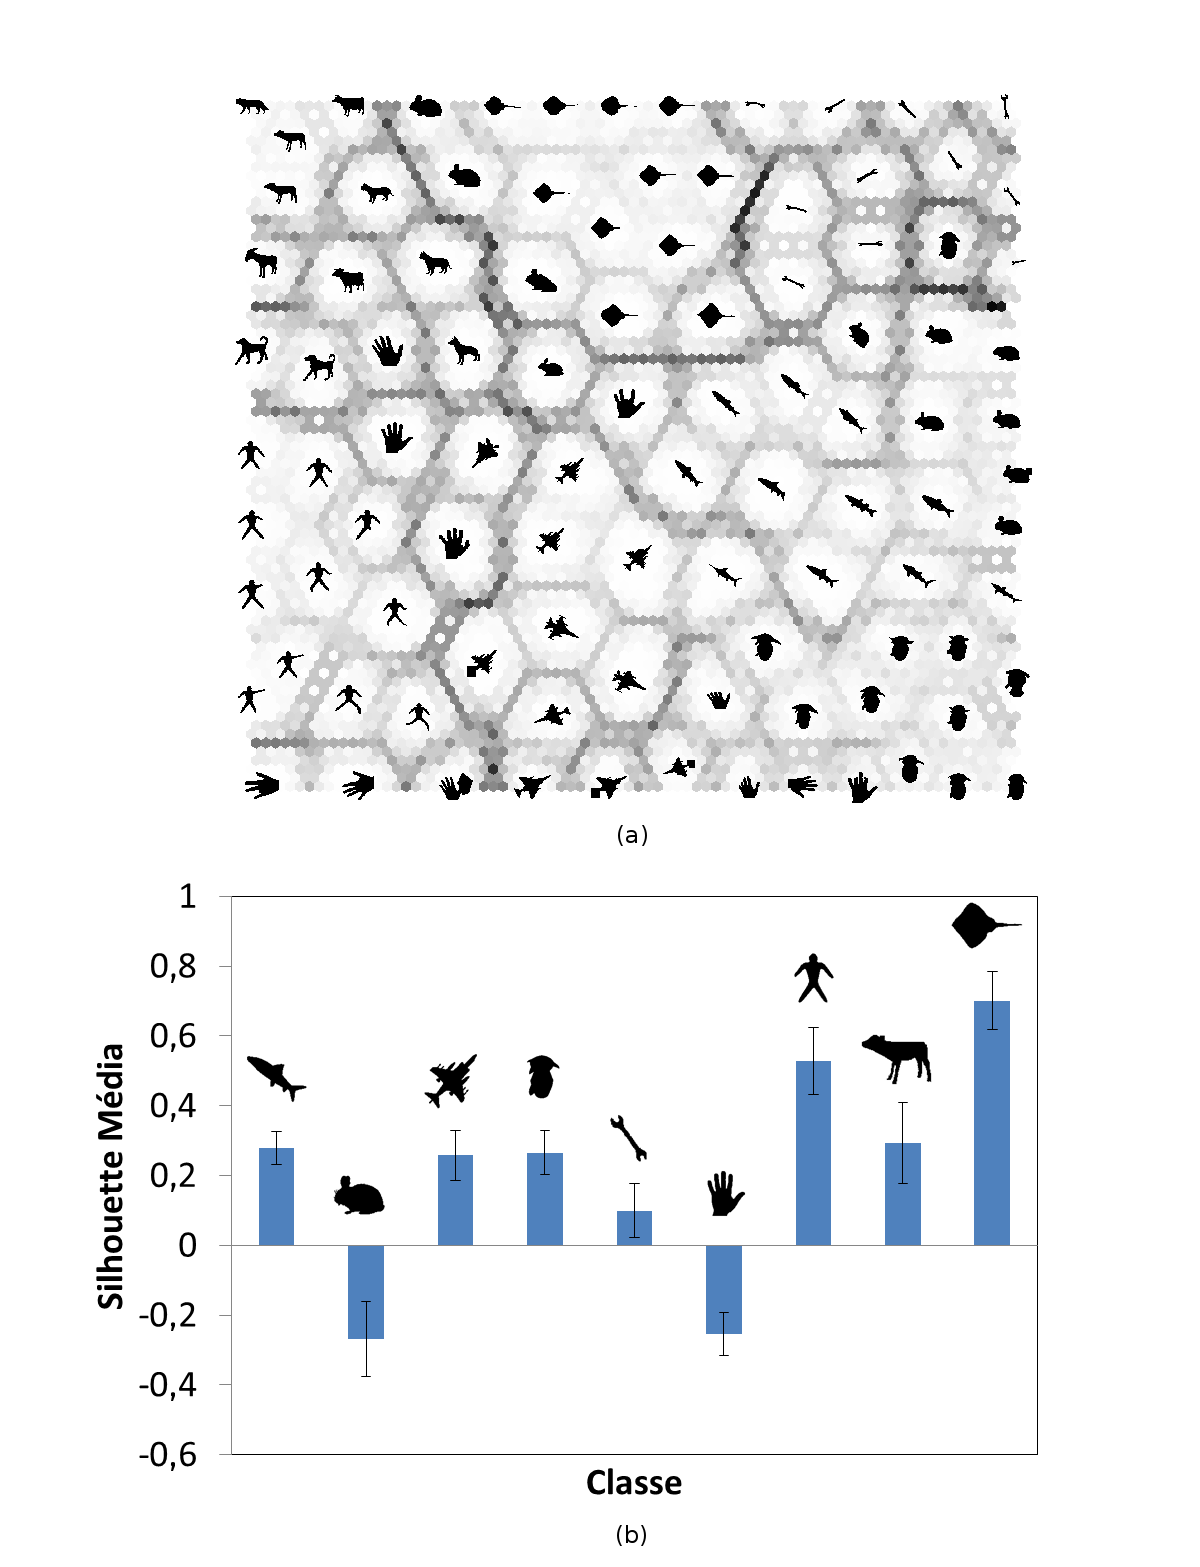
\includegraphics[width=\textwidth]{dfm99.png}
\end{figure}

\begin{figure}
 \caption{\label{fig:dfm216} (a) Matriz-U para as formas da base Kimia216 representadas com o descritor dimensão fractal multiescala. (b) \textit{Silhouette} média por classe obtida a partir do referido descritor.}
  \centering
  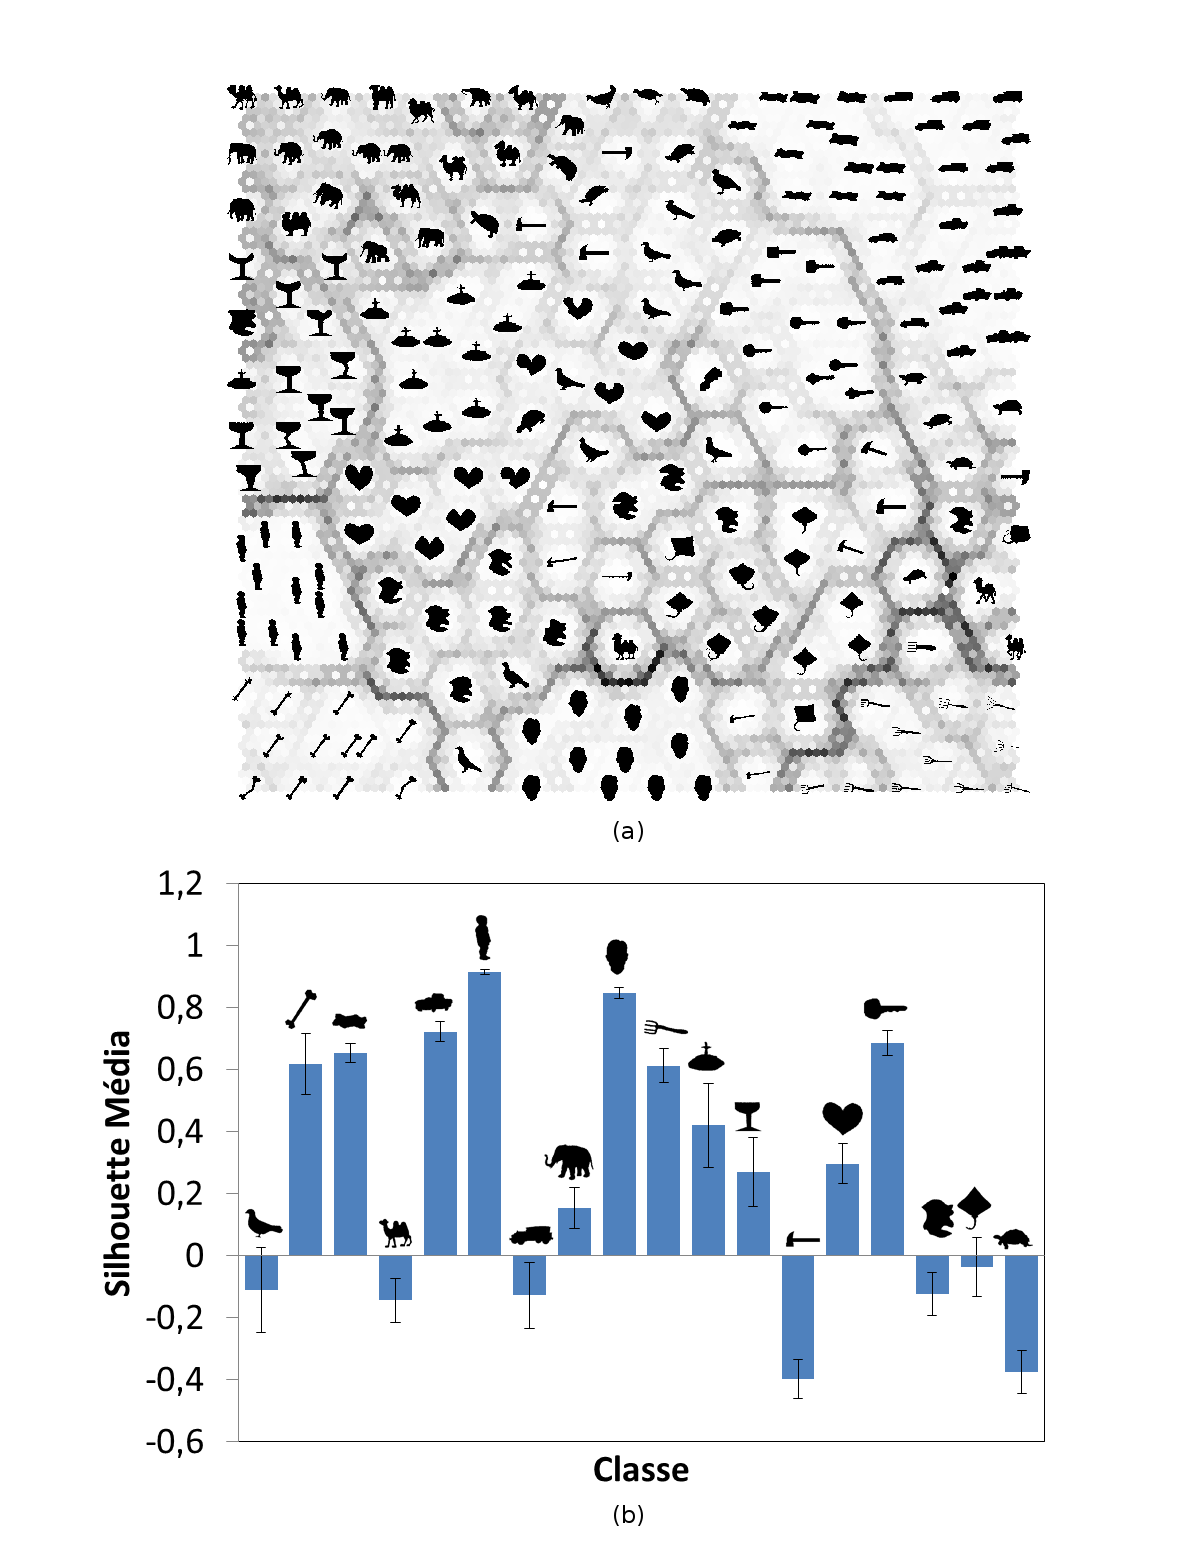
\includegraphics[width=\textwidth]{dfm216.png}
\end{figure}

\begin{figure}
 \caption{\label{fig:nmbe99} (a) Matriz-U para as formas da base Kimia99 representadas com o descritor energia de dobramento multiescala. (b) \textit{Silhouette }média por classe obtida a partir do referido descritor.}
  \centering
  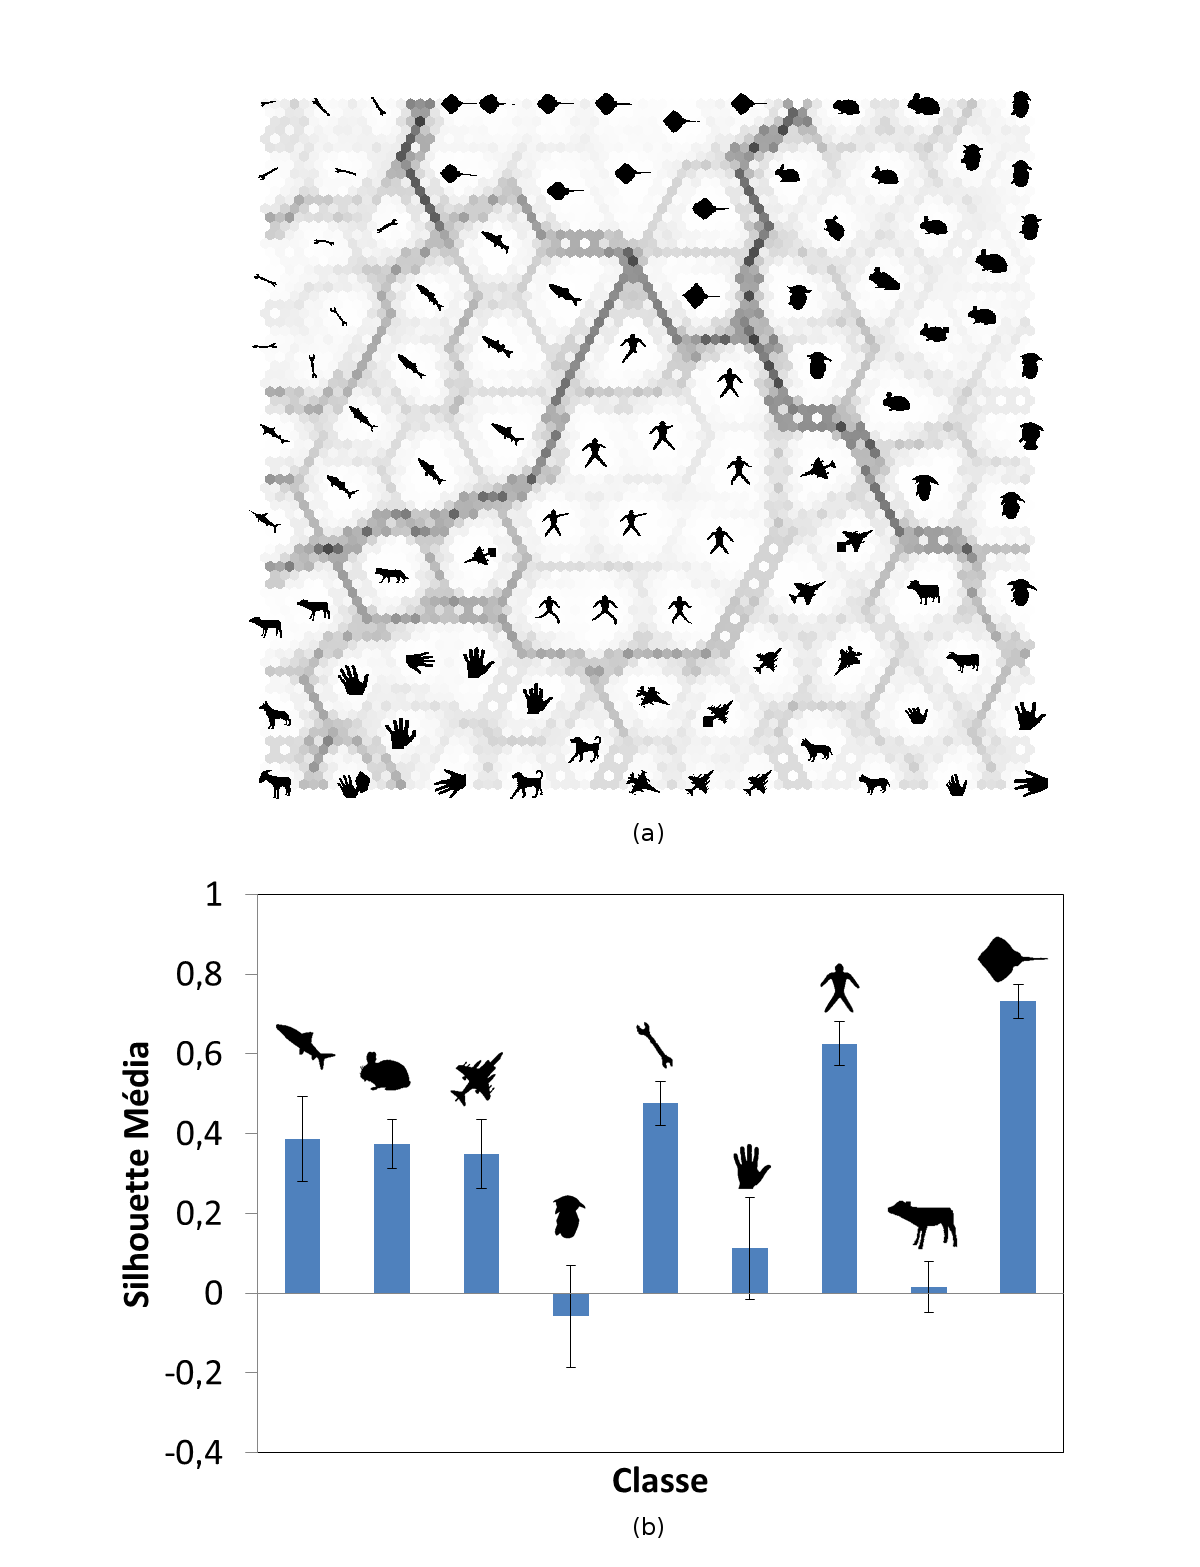
\includegraphics[width=\textwidth]{nmbe99.png}
\end{figure}

\begin{figure}
 \caption{\label{fig:nmbe216} (a) Matriz-U para as formas da base Kimia216 representadas com o descritor energia de dobramento multiescala. (b) Silhouette média por classe aferida a partir do descritor}
  \centering
  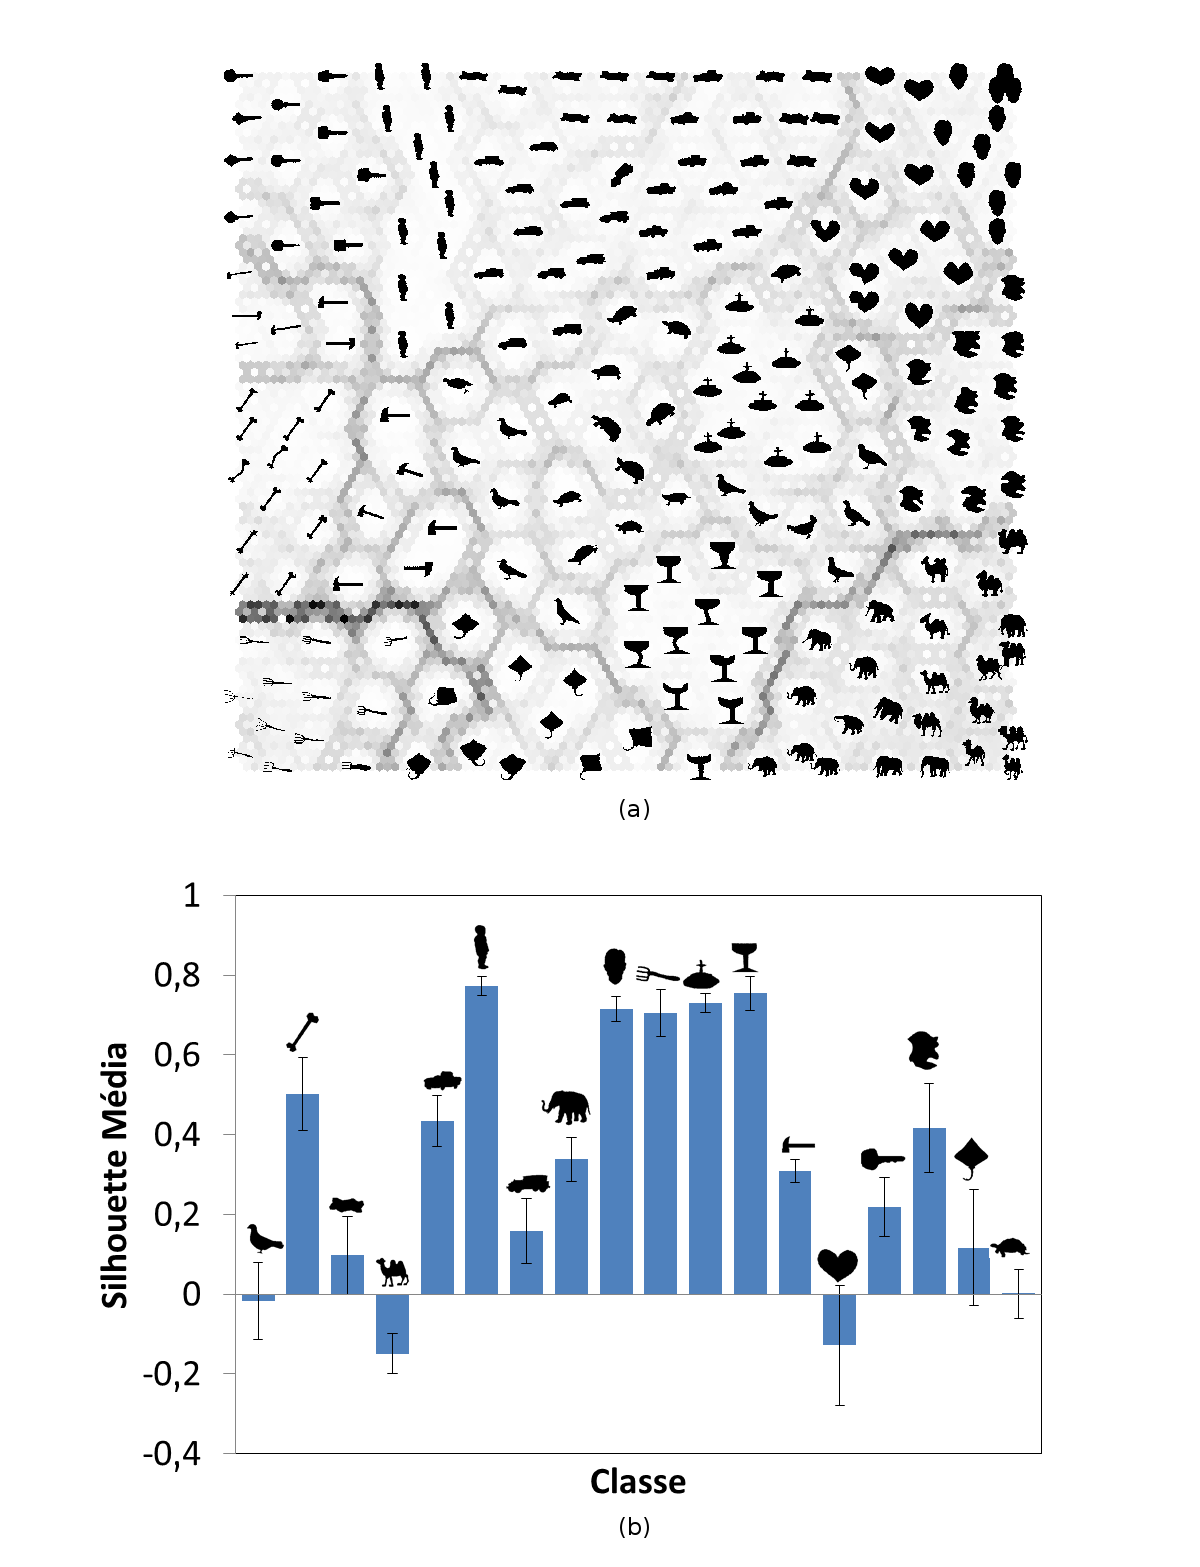
\includegraphics[width=\textwidth]{nmbe216.png}
\end{figure}


\begin{comment}
\begin{figure}
 \caption{\label{fig:edif99} (a) Matriz-U para as formas da base Kimia99 representadas com o descritor entropia multiescala. (b) Silhouette média por classe aferida a partir do descritor}
  \centering
  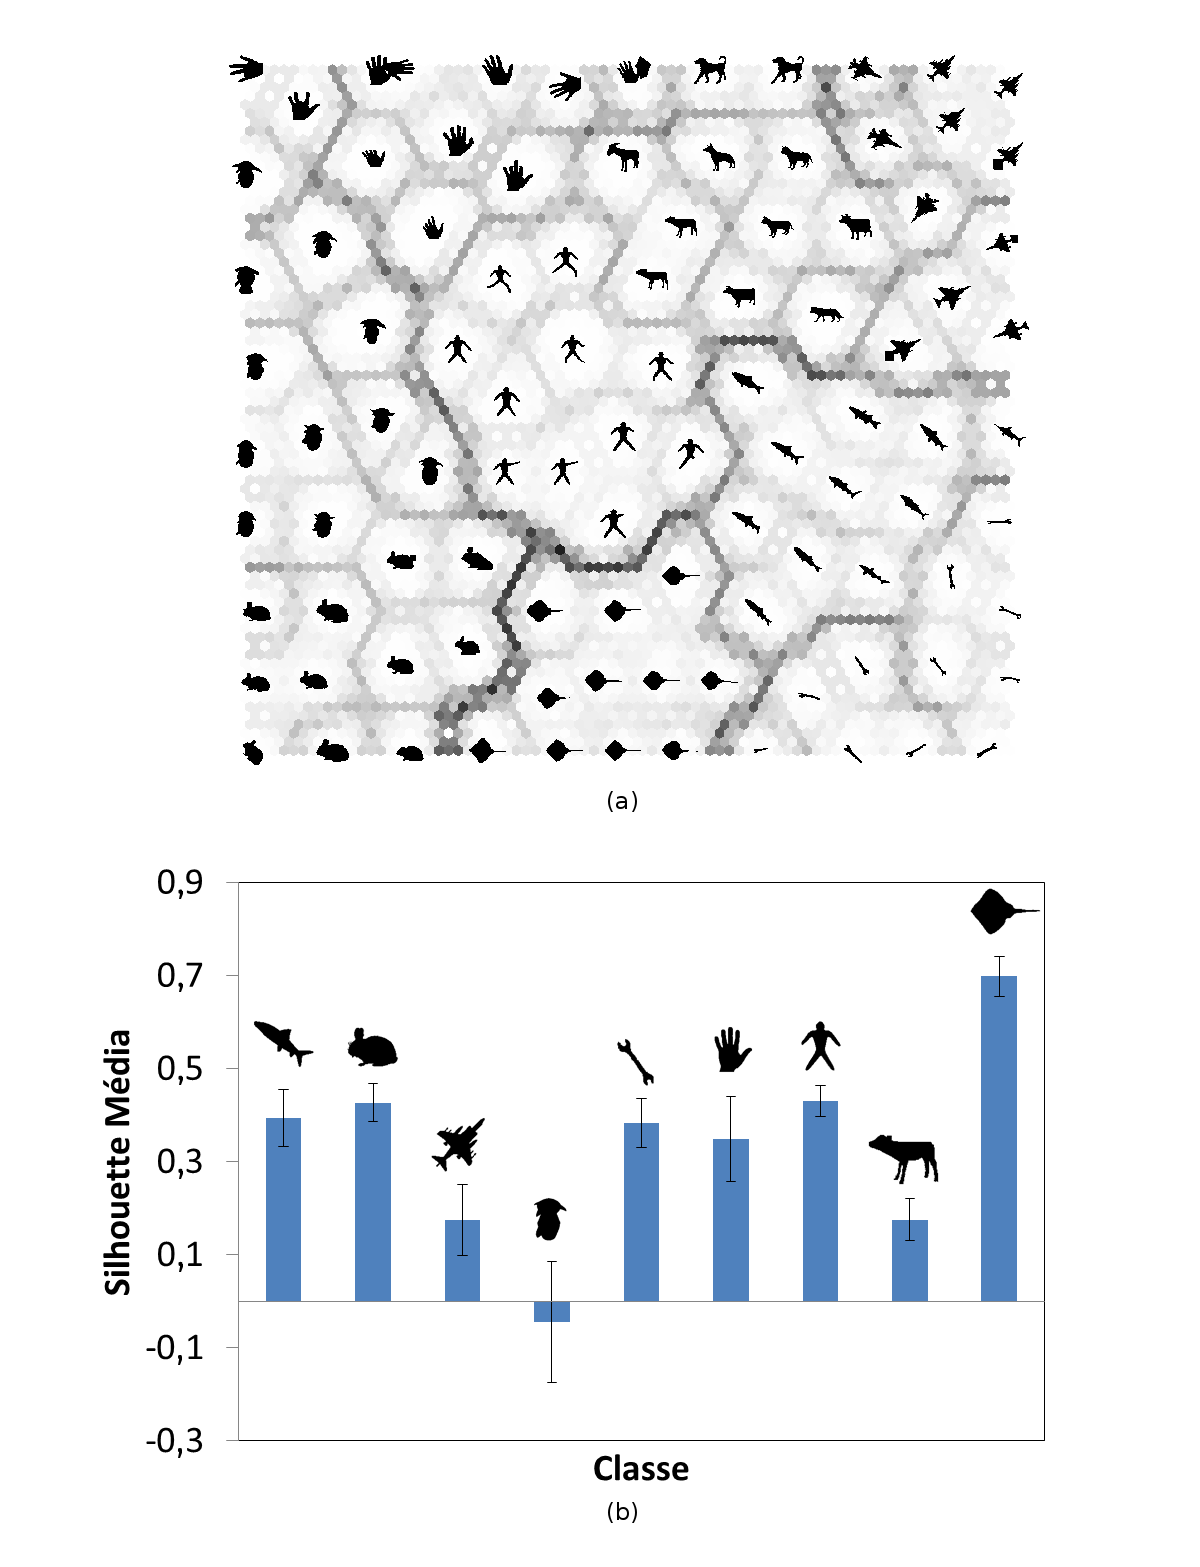
\includegraphics[width=\textwidth]{ediferencial99.png}
\end{figure}

\begin{figure}
 \caption{\label{fig:edif216} (a) Matriz-U para as formas da base Kimia216 representadas com o descritor entropia multiescala. (b) Silhouette média por classe aferida a partir do descritor}
  \centering
  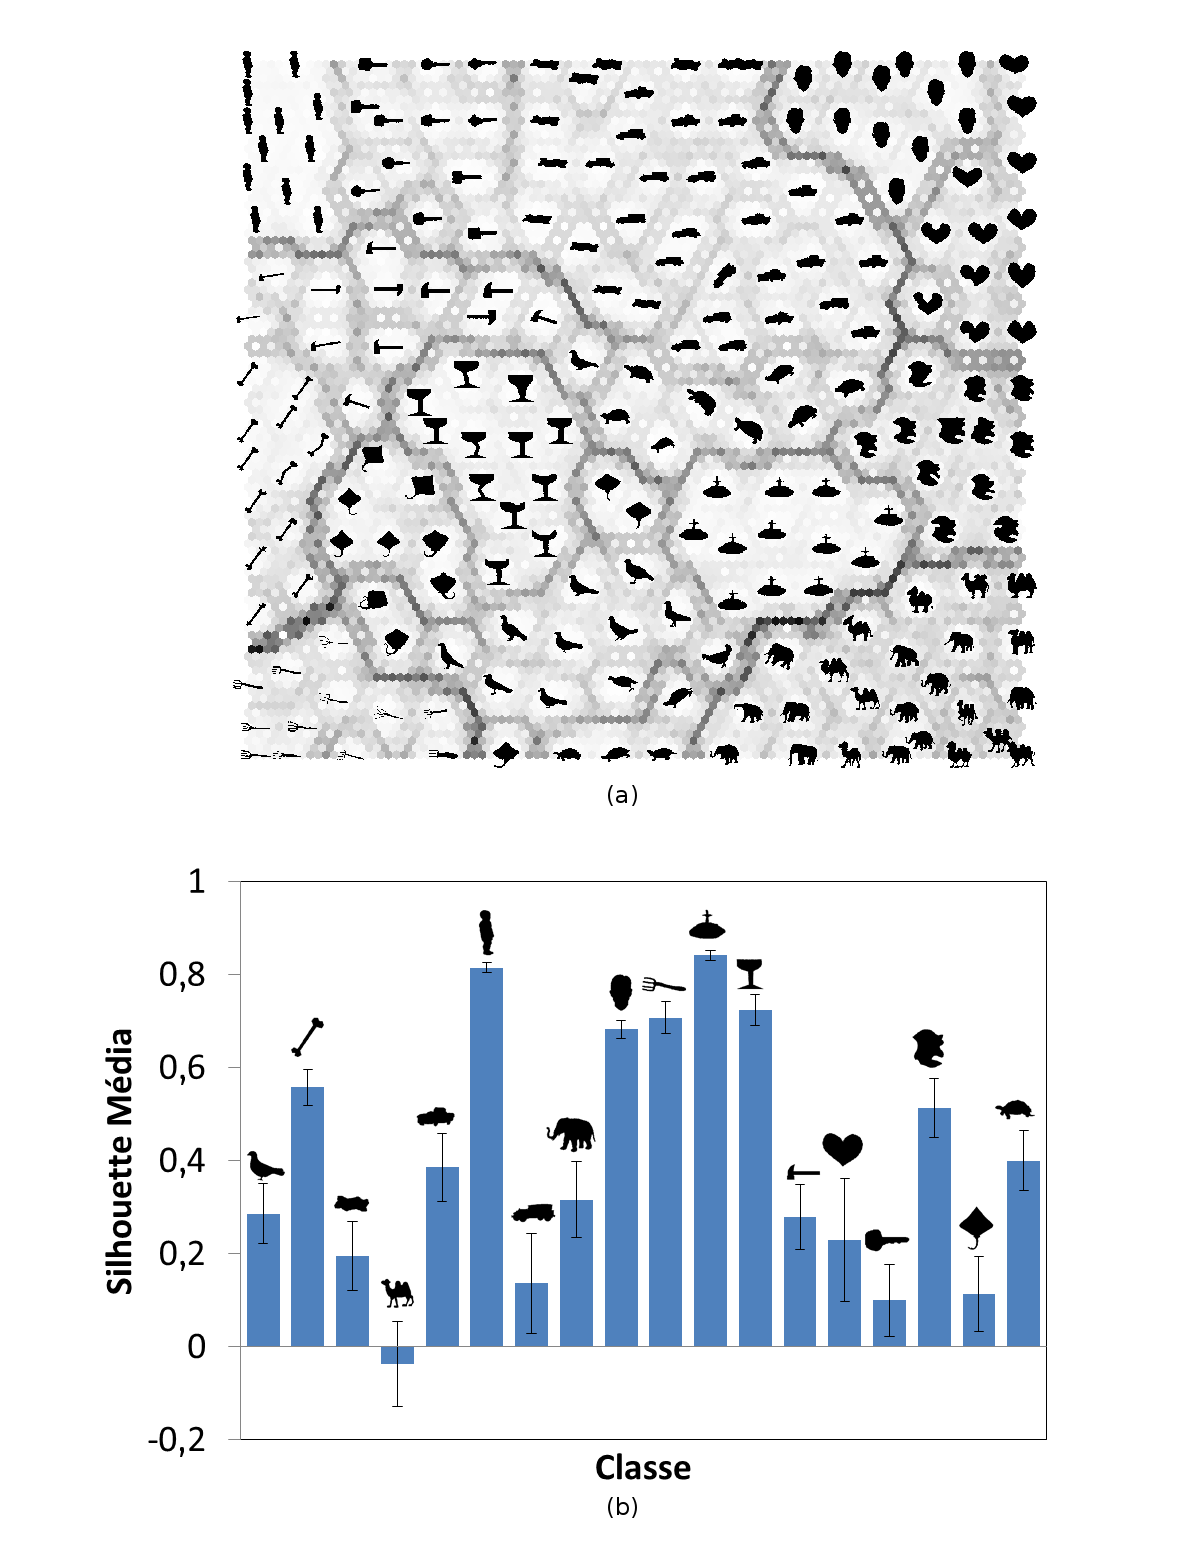
\includegraphics[width=\textwidth]{ediferencial216.png}
\end{figure}

\begin{figure}
 \caption{\label{fig:edis99} (a) Matriz-U para as formas da base Kimia99 representadas com o descritor entropia multiescala. (b) Silhouette média por classe aferida a partir do descritor}
  \centering
  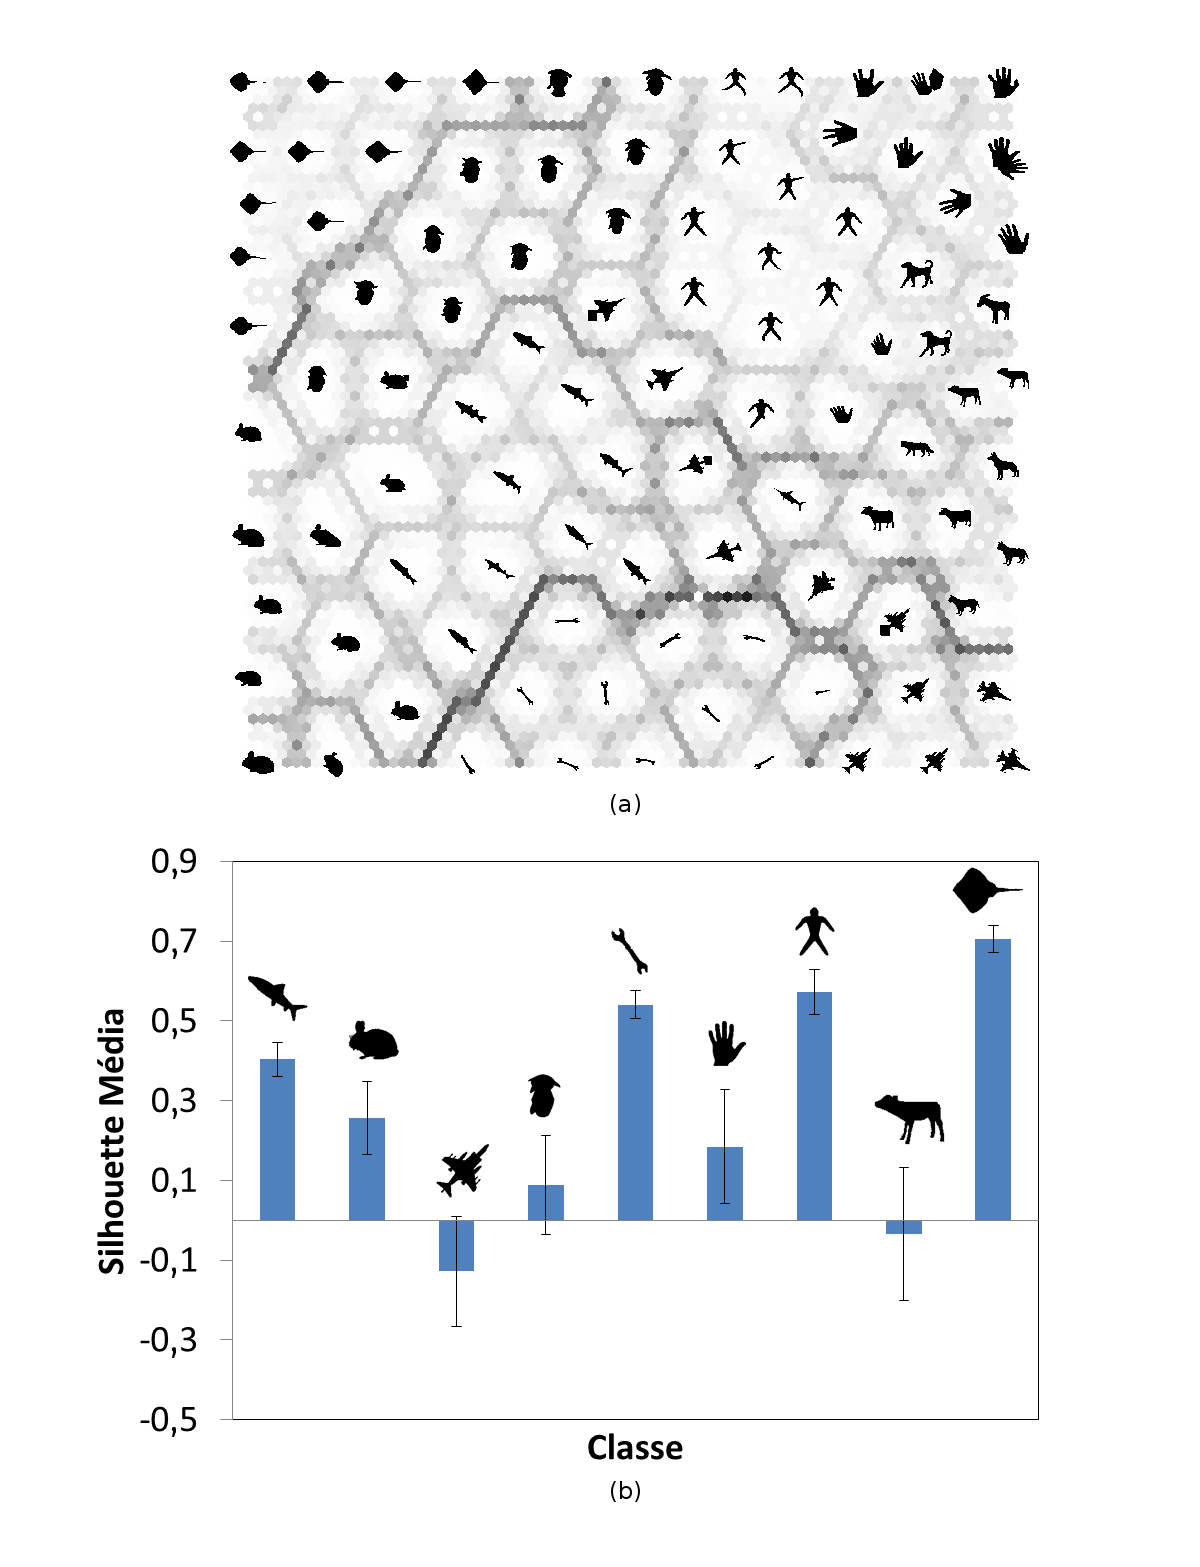
\includegraphics[width=\textwidth]{ediscreta99.png}
\end{figure}

\begin{figure}
 \caption{\label{fig:edis216} (a) Matriz-U para as formas da base Kimia216 representadas com o descritor entropia multiescala. (b) Silhouette média por classe aferida a partir do descritor}
  \centering
  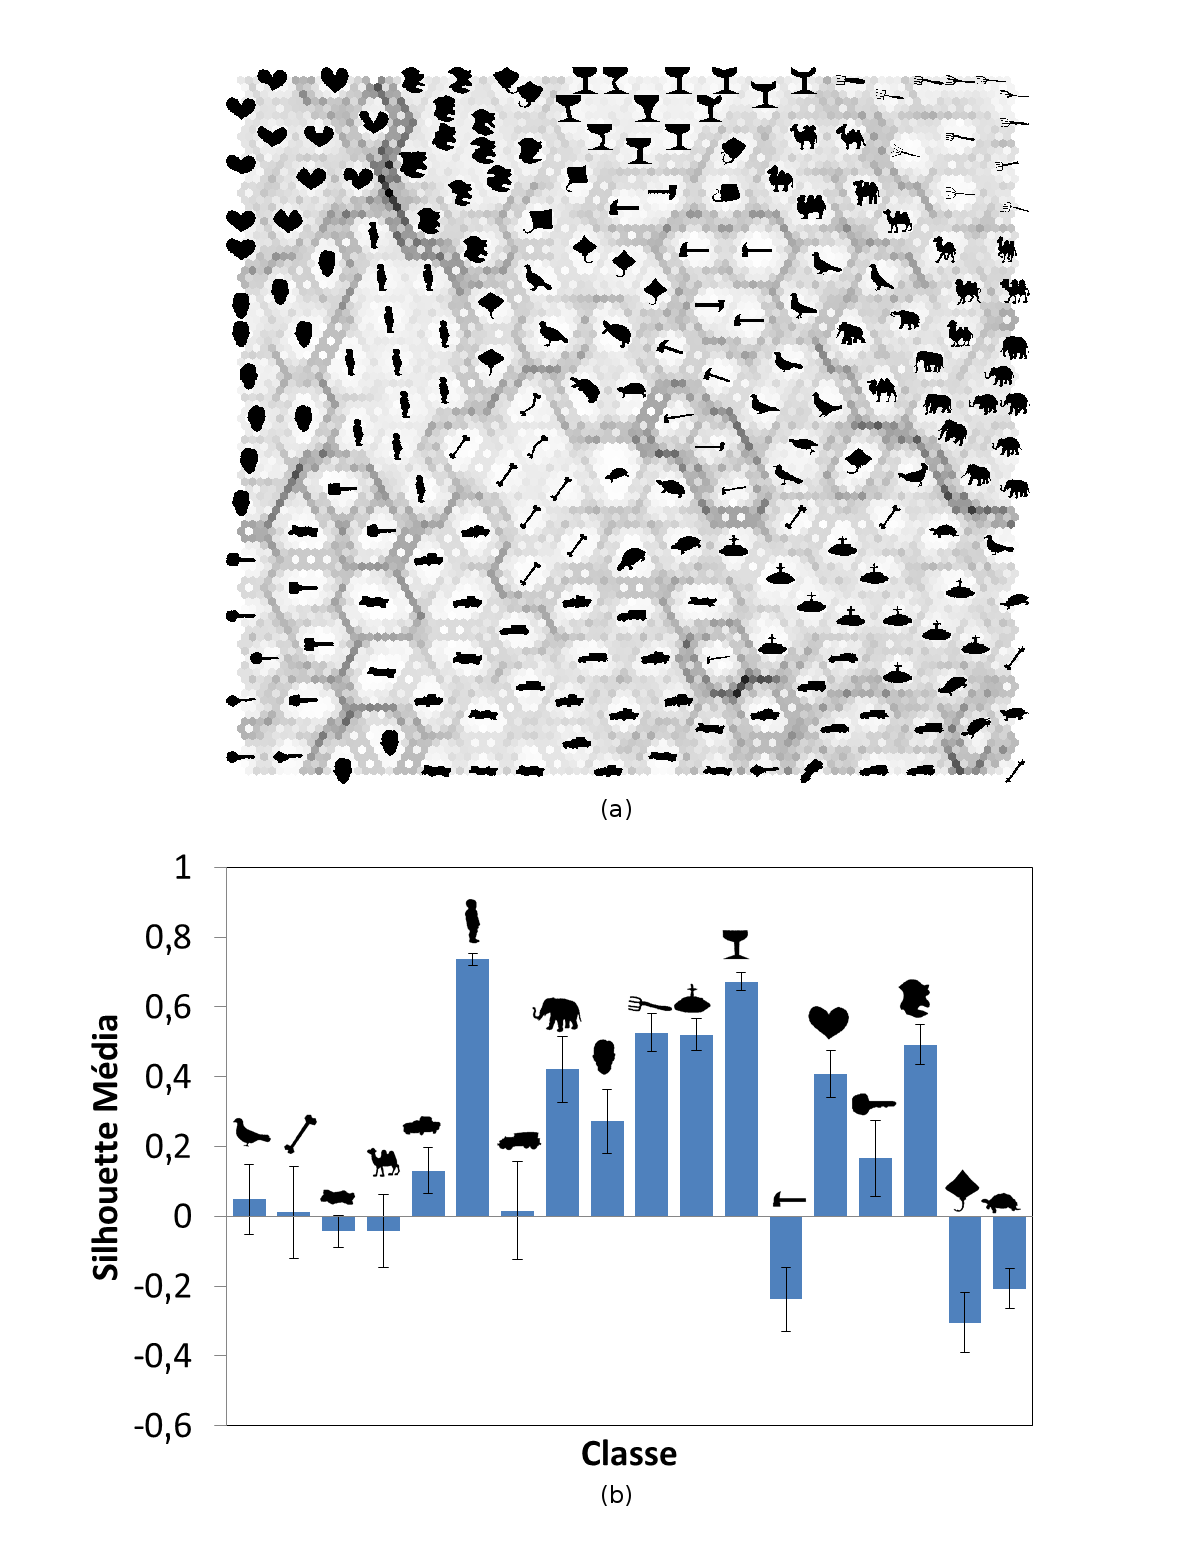
\includegraphics[width=\textwidth]{ediscreta216.png}
\end{figure}

\subsection{\emph{NMBE} e \emph{DFM}}
Os experimentos de avaliação de desempenho dos descritores produziram como saída as matrizes-U que estão apresentadas na Figuras \ref{fig:nmbe_som_map}, \ref{fig:mfd_som_map} e  \ref{fig:som_kimia_216}. Nas Figuras \ref{fig:nmbe_som_map} e \ref{fig:mfd_som_map}, as regiões delimitadas com linhas tracejadas correspondem as classes de formas com os maiores valores médios da medida Silhouette (Figuras \ref{fig:silhouette}a e \ref{fig:silhouette}b). Nesses casos pode-se deduzir que ambos os descritores foram capazes de caracterizar corretamente estas classes de formas.

Já os grupos delimitados com linhas contínuas referem-se às classes de formas com os menores valores de Silhouette média. De fato, as formas dessas classes aparecem nas matrizes-U dispersas em sub-grupos, que é um indicativo que ambos os descritores falharam em caracterizá-las adequadamente.
  
As Figuras \ref{fig:dude_tool_mfd} e \ref{fig:dude_tool_nmbe} mostram objetos das classes de formas de humanos e ferramentas. Ambos os descritores foram capazes de discriminar os objetos das referidas classes, como evidenciado nos gráficos apresentados. As matrizes-U (Figuras \ref{fig:nmbe_som_map} e \ref{fig:mfd_som_map}) também confirmam esse resultado exibindo, para essas classes de formas, homogeneidade intra-classe e separabilidade inter-classes. Logo, concluímos que estes descritores são efetivos em representar formas para o reconhecimento de padrões em aplicações \emph{CBIR}.

Também evidenciamos nas Figuras \ref{fig:mfd_som_map} e \ref{fig:nmbe_som_map} que o descritor \emph{DFM} apresentou maior dispersão inter-classe para as formas de humanos que o descritor \emph{NMBE}. Essa observação é consistente com os resultados obtidos através da medida \emph{Silhouete}, aonde o valor dessa medida para formas humanas descritas com a \emph{DFM} é menor do que o valor para essas mesmas formas descritas com a \emph{NMBE}.

Ademais, os sinais em linhas tracejadas vermelhas e em linhas contínuas azuis, apresentados nas Figuras \ref{fig:dude_tool_mfd} e \ref{fig:dude_tool_nmbe}, mostram que o descritor \emph{NMBE} é mais robusto a diferenças intra-classe que o descritor \emph{DFM}. Nesses gráficos, as formas pertencentes a mesma classe que o descritor representa seguindo um mesmo padrão apresentam-se próximas umas das outras na matriz-U, enquanto as formas que o descritor representa divergindo do padrão são mapeadas na matriz-U distantes dos grupo correspondente. Exemplos desta última condição são as formas humanas rotuladas como $2$ e $4$ nas Figuras \ref{fig:dude_tool_mfd} e \ref{fig:dude_tool_nmbe}.


Furthermore, there is a larger variation among tools descriptions in the graphs of  the figure \ref{fig:descritores}a than the  variations observed in the graphs of the figure \ref{fig:descritores}b. Coherently, the corresponding shapes appears in the U-matrix more dispersed  for the \emph{MFD} description than for the \emph{NMBE} description.

\begin{figure}[h!]
  \caption{\label{fig:nmbe_som_map} Matriz-U para as formas da base Kimia99 representadas com o descritor Energia de dobramento multiescala.}
  \centering
  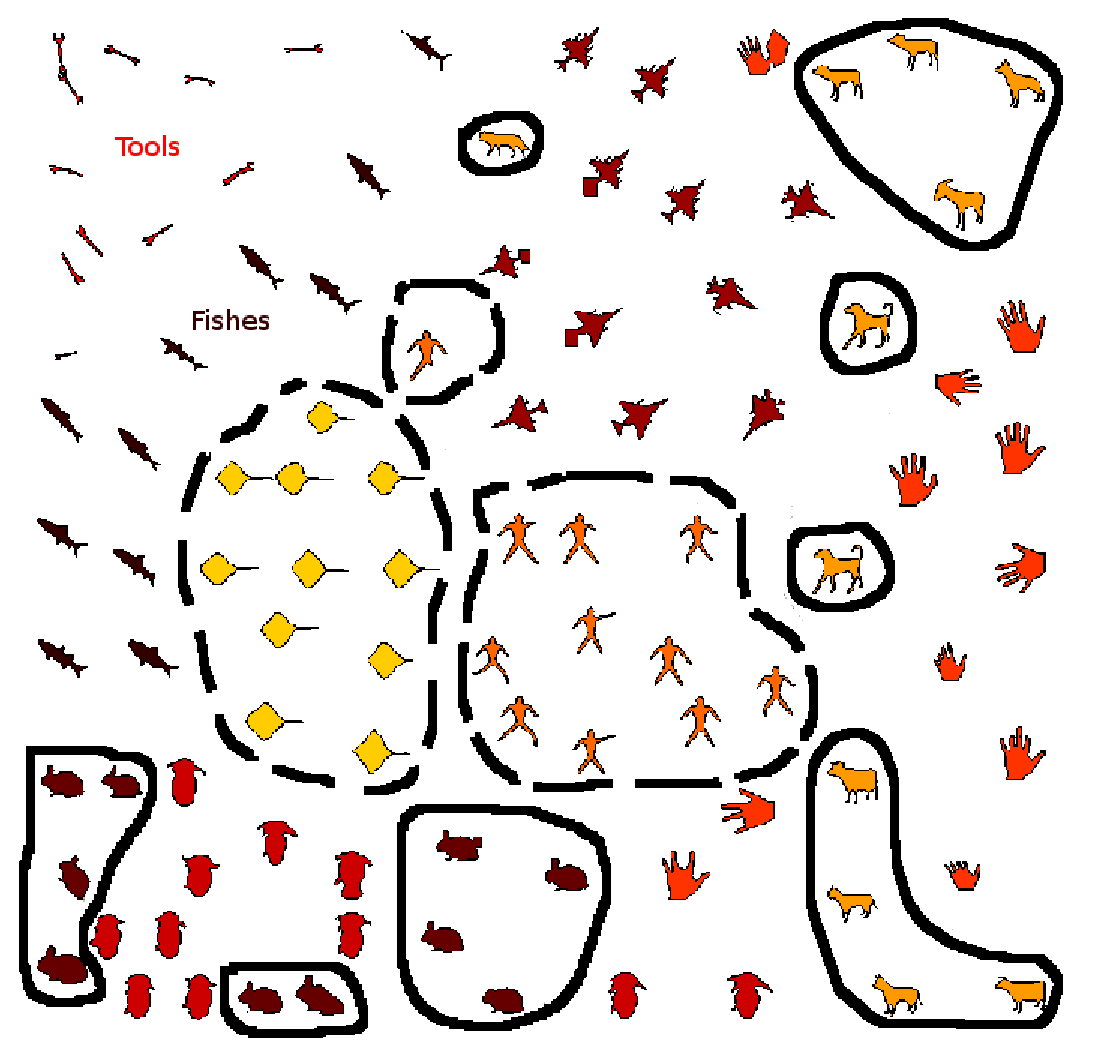
\includegraphics[width=0.5\textwidth]{nmbe_som_map_v4.eps}
\end{figure}

\begin{figure}[h!]
  \caption{\label{fig:mfd_som_map} Matriz-U para as formas da base Kimia99 representadas com o descritor Dimensão fractal multiescala.}
  \centering
  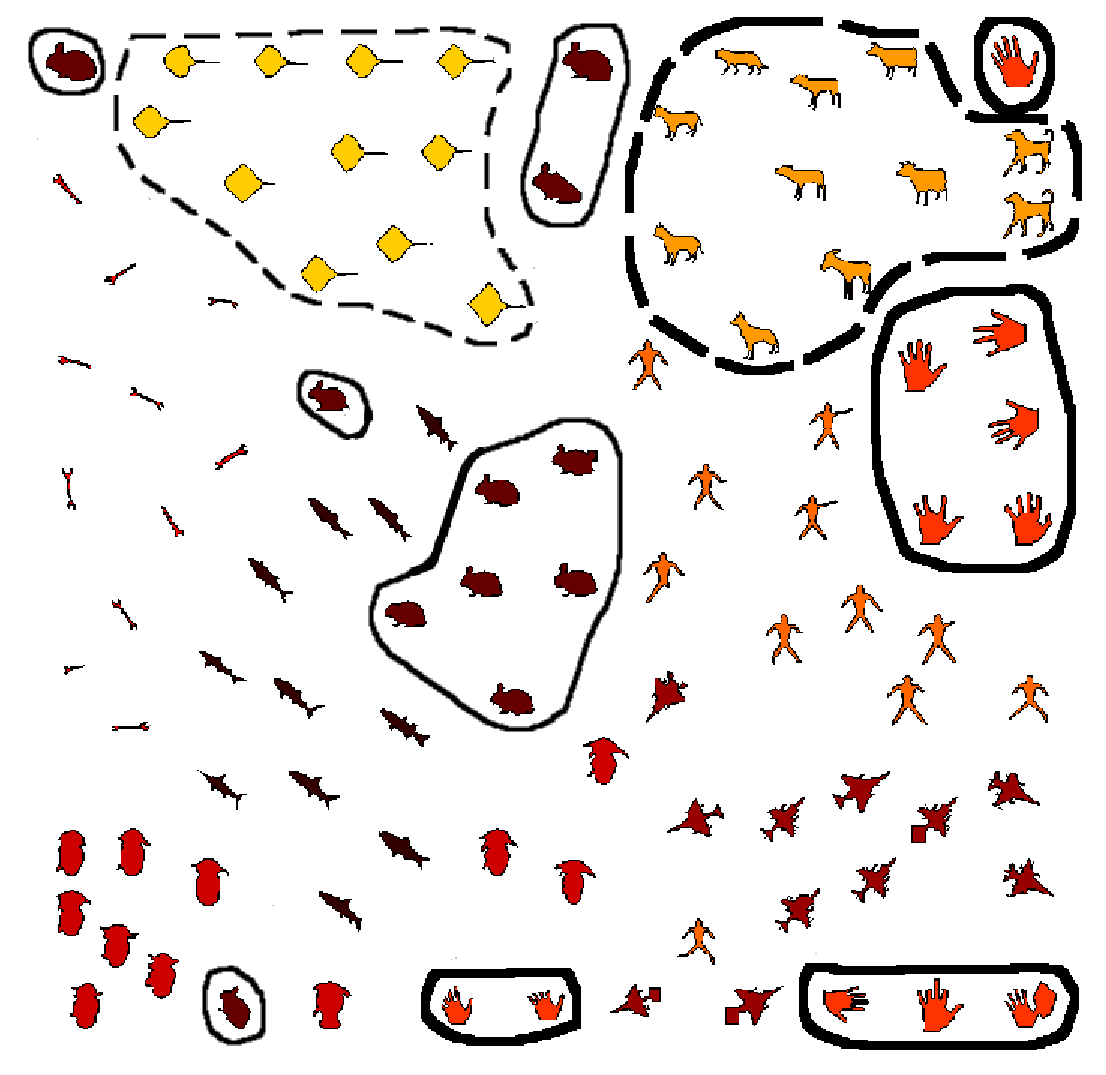
\includegraphics[width=0.5\textwidth]{mfd_som_map_v3.eps}
\end{figure}
  
\begin{figure}[h!]  \caption{\label{fig:som_kimia_216} Para o descritor energia de dobramento multiescala e a base Kimia-216: (a) Matriz-U. (b) Alguns resultados de recuperação de formas pelo conteúdo.}
  \centering
  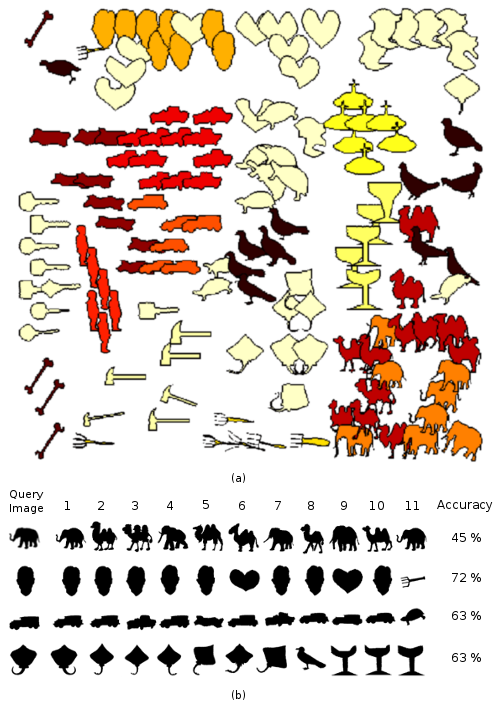
\includegraphics[width=0.5\textwidth]{retr_som_kimia216_v2.png}
\end{figure}

Já a Figura \ref{fig:som_kimia_216}a apresenta os resultados da visualização das formas da base Kimia-216 representadas através do descritor \emph{NMBE}. No canto inferior direito desta figura observamos que o descritor confunde formas dos elefantes com as dos camelos. Essa confusão aparece também no experimento de recuperação de formas pelo conteúdo (Figura \ref{fig:som_kimia_216}b), em que uma dentre as formas dos elefantes é utilizada como protótipo para se recuperar as onze formas mais similares ao protótipo na referida base.

Analogamente, no canto superior esquerdo da Figura \ref{fig:som_kimia_216}a, há confusão entre os agrupamentos das formas das faces e dos corações, bem como a presença duma forma de garfo. Na segunda linha da Figura \ref{fig:som_kimia_216}b observamos a presença dessas formas indesejáveis no experimento de recuperação de formas quando uma forma de face é apresentada como protótipo. 

Os demais resultados de recuperação de formas, apresentados na Figura \ref{fig:som_kimia_216}b, também estão coerentes com as observações da matriz-U. Nessa última podemos observar que o grupo das formas das arraias são mapeadas vizinhas aos grupos das formas dos cálices e dos pássaros, o que resulta no aparecimento das formas dessas últimas classes quando se realiza a recuperação de arraias. 

Outro aspecto importante de ser observado é que  grupos de formas com similaridades grosseiras encontram-se mapeados próximos uns dos outros na matriz-U. Formas alongadas, por exemplo, estão organizadas na parte inferior esquerda da Figura \ref{fig:som_kimia_216}a, enquanto formas arredondadas encontram-se na parte superior. Outros exemplos incluem os seguintes grupos: chaves e crianças (esquerda da figura), carros e tijolos, tartarugas e pássaros, cálices e sepulturas. 

\begin{figure}[h!]
  \caption{\label{fig:silhouette} Silhouette média por classe aferida, com a base Kimia-99, para os descritores (a) Dimensão fractal multiescala; (b) Energia de dobramento multiescala.}
  \centering
  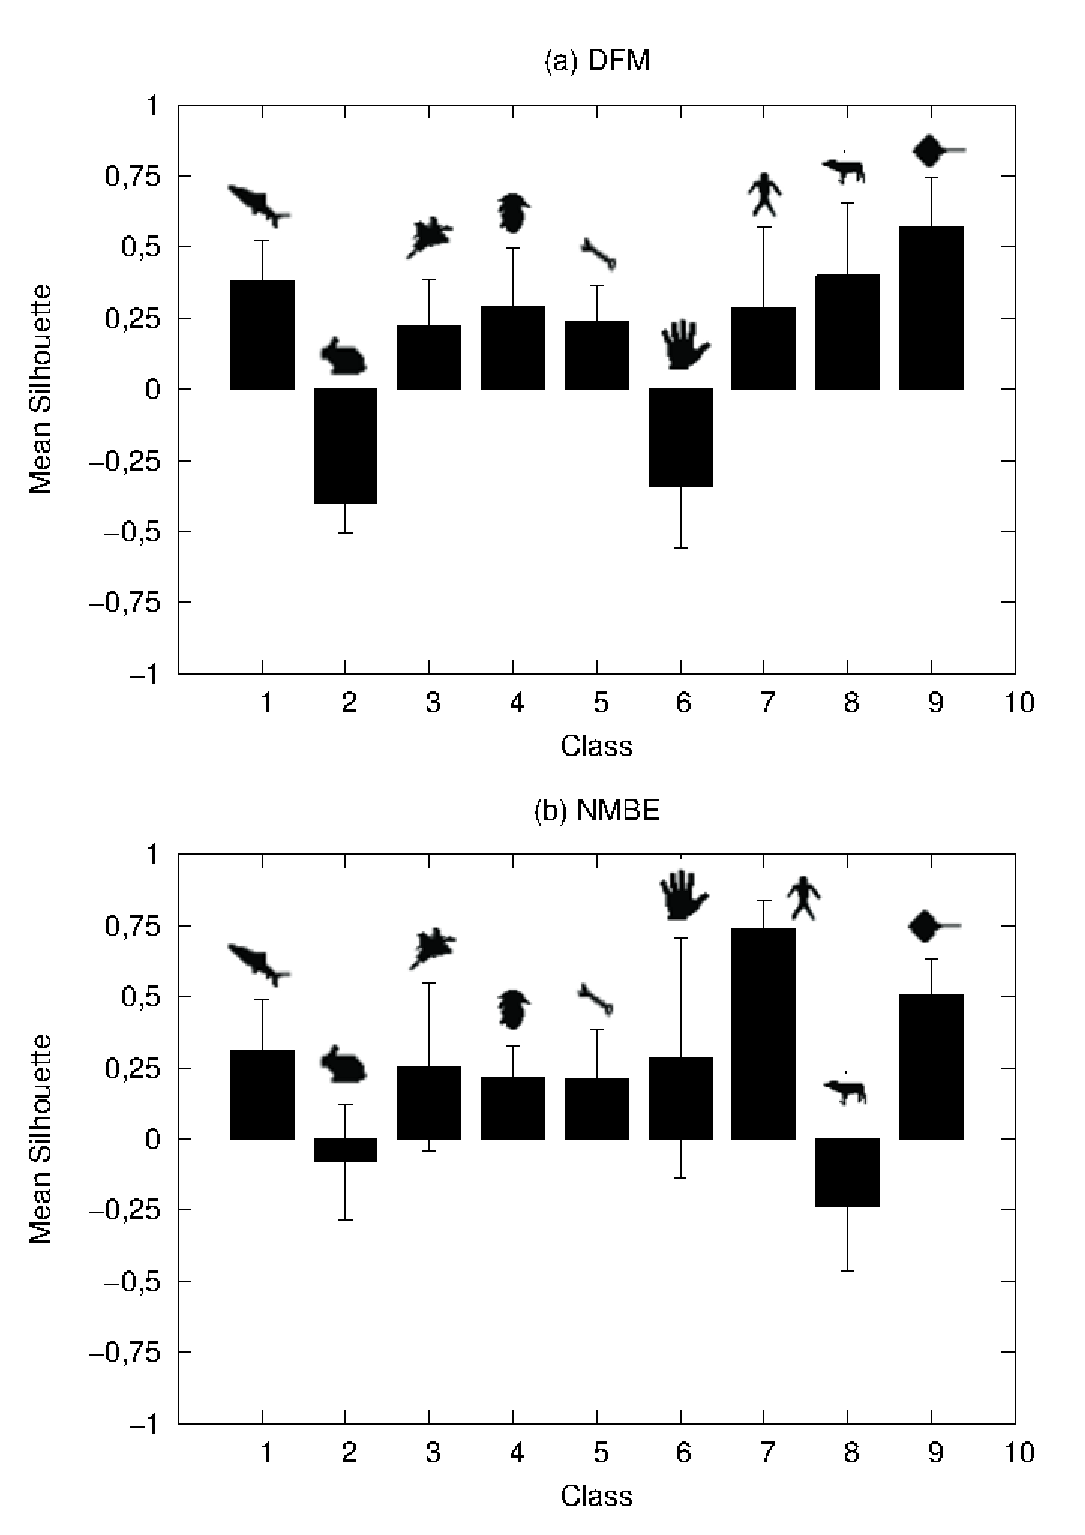
\includegraphics[width=0.5\textwidth]{resultado_silhouette.eps}
\end{figure}

\begin{figure}[h!]
  \caption{\label{fig:dude_tool_mfd}   Vetores de características calculados para amostras das formas de humanos e de ferramentas com o descritor dimensão fractal multiescala.}
  \centering
  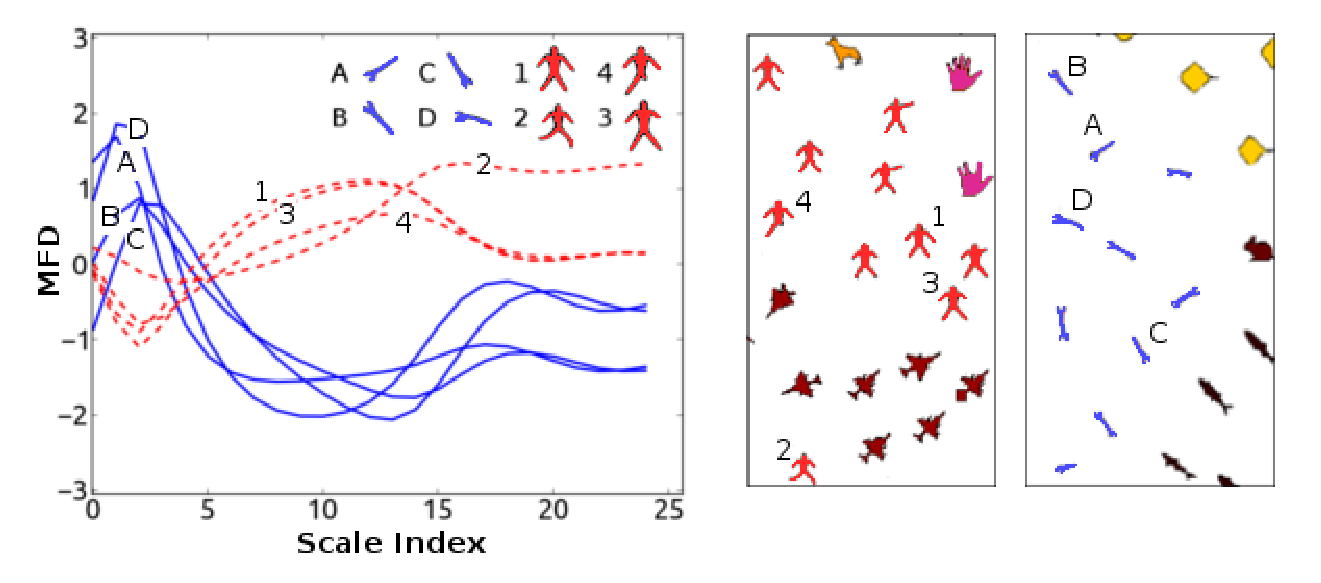
\includegraphics[width=0.75\textwidth]{dude_tool_mfd_v6.eps}
\end{figure}

\begin{figure}[h!]
  \caption{\label{fig:dude_tool_nmbe} Vetores de características calculados para amostras das formas de humanos e de ferramentes com o descritor energia de dobramento multiescala.}
  \centering
  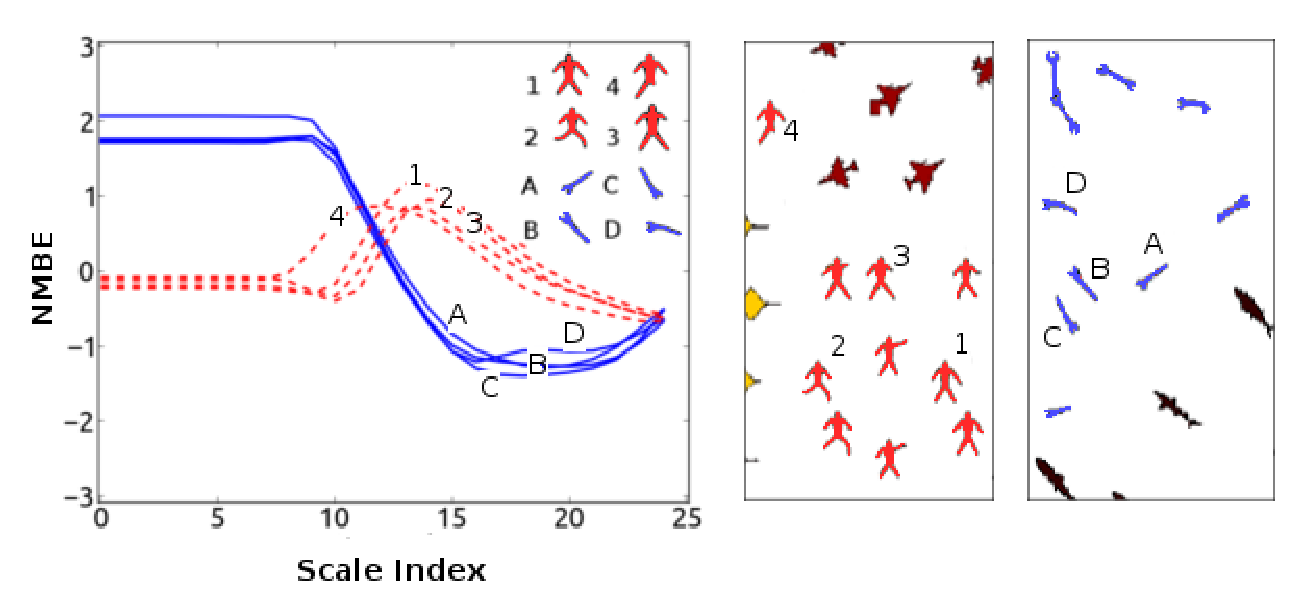
\includegraphics[width=0.75\textwidth]{dude_tool_nmbe_v6.eps}
\end{figure}

\subsection{Entropia diferencial da curvatura multiescala}

A visualização de dados obtida para características extraídas com o descritor entropia diferencial da curvatura multiescala, para a base Kimia-99, está apresentada na Figura \ref{fig:edif99}a. Nesta figura observamos a Matriz-U, em tons de cinza, sobreposta às figuras das formas nas posições mapeadas pela rede SOM.

As células escuras formam contornos que delimitam fronteiras existentes entre agrupamentos de formas, pois estas células indicam a existência duma relação de separação entre as formas em suas vizinhanças. Já as células em linhas claras indicam maior proximidade entre as formas e suas vizinhanças.

Podemos inferir que o descritor representou adequadamente as formas das classes de humanos, arraias, peixes, ferramentas e coelhos. Isso porque, nestes casos, o descritor apresentou uma representação compacta, agrupando próximas as formas de uma mesma classe, e propiciando separabilidade entre os agrupamentos estabelecidos. A medida Silhouette média por classe, apresentada na Figura \ref{fig:edif99}b, corrobora nossas observações, pois as referidas classes são as que apresentam os valores de Silhouette média mais positivos e com pequeno desvio padrão.  

Por outro lado, o descritor falhou em representar as formas das classes de animais quadrúpedes, aviões e extra terrestres. Isso porque, nesses casos, não se consegue identificar na matriz-U fronteiras claras que estabeleçam um único agrupamento das formas de uma mesma classe. Em outras palavras, formas dessas classes encontram-se separadas umas das outras ou dispersas em sub-grupos delimitados por pequenas fronteiras. Esses casos são os que apresentam a medida Silhouette média por classe com os menores valores e os maiores desvios padrão. 

Já na Figura \ref{fig:edif216}a temos a visualização da matriz-U para as características extraídas das formas da base Kimia-216. Nesta observamos, bem delimitados por linhas escuras, diversos agrupamentos  representados corretamente pelo descritor. Dentre esses, destacamos os agrupamentos cujas fronteiras de separação intra-classe são de baixo contraste e cujas fronteiras de separação inter-classe são bem contrastadas (faces, garfos, sepulturas, cálices e crianças). Esses são os  agrupamentos que apresentaram os maiores valores de \emph{Silhouette} média na Figura \ref{fig:edif216}b, o que é um resultado esperado, uma vez que o descritor representou as formas desses grupos de forma compacta e em agrupamentos bem separados.

\begin{figure}
\caption{\label{fig:edif_som_map} Matriz-U para as formas da base Kimia99 representadas com o descritor Entropia diferencial da curvatura multiescala.}
  \centering
  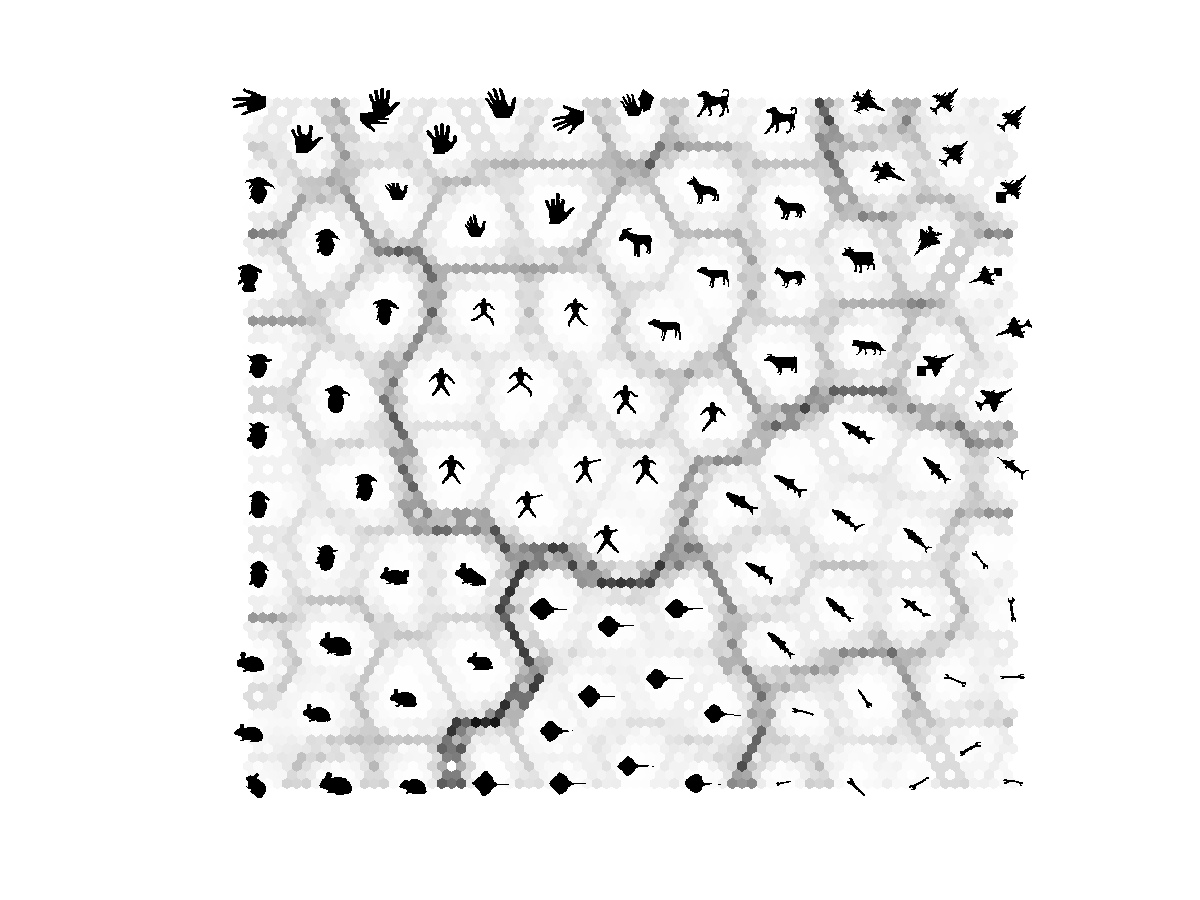
\includegraphics[width=\textwidth]{ediferencial_N5_formas.png}
 \end{figure}

\begin{figure}
\caption{\label{fig:silhouette_ediferencial} Silhouette média por classe aferida, com a base Kimia-99, para o descritor entropia diferencial da curvatura multiescala.}
  \centering
  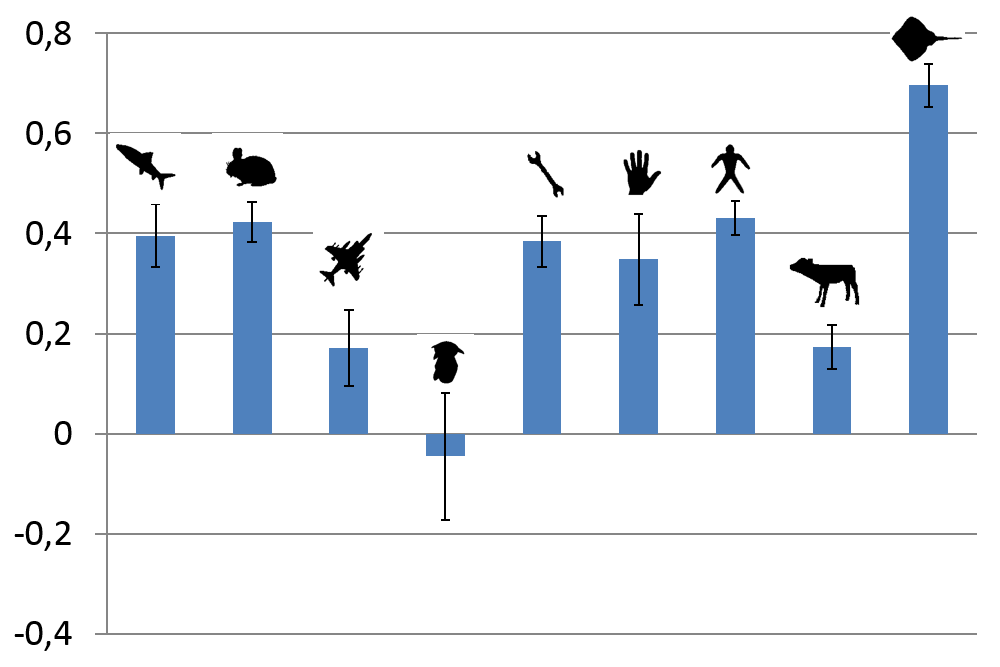
\includegraphics[width=0.75\textwidth]{ediferencial_silhouette_N5.png}
\end{figure}

\begin{figure}[h!]
  \caption{\label{fig:som_nmbe} Visualização dos dados obtida com o mapa auto-organizável de Kohonen para a descrição \emph{NMBE}.}
  \centering
  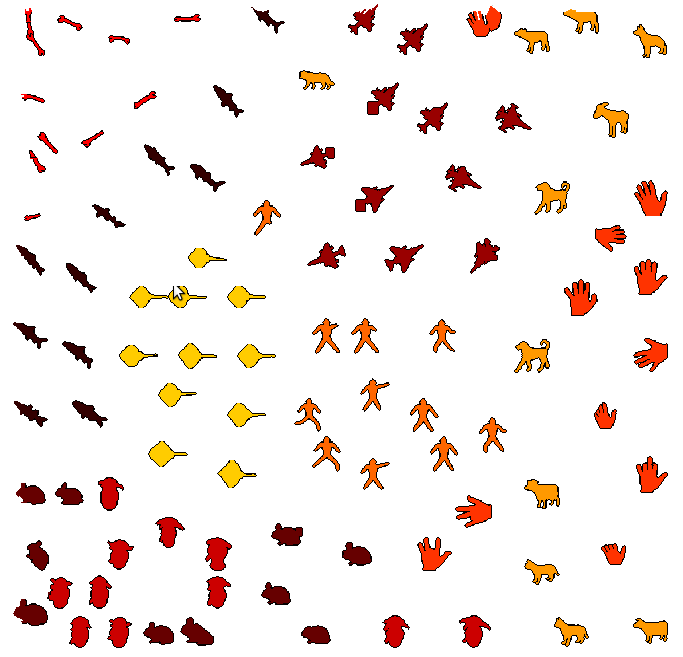
\includegraphics[width=0.5\textwidth]{mapa_som_descritor_nmbe.png}
\end{figure}

\begin{figure}[h!]
  \caption{\label{fig:som_dfm} Visualização dos dados obtida com o mapa auto-organizável de Kohonen para a descrição \emph{NMBE}.}
  \centering
  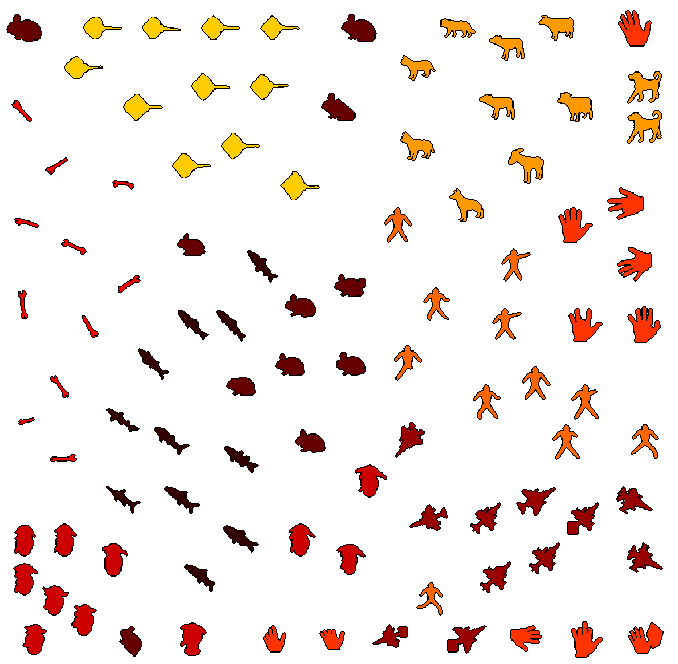
\includegraphics[width=0.5\textwidth]{mapa_som_descritor_dfm.png}
\end{figure}

\section{Recuperação de imagens pelo conteúdo}

\begin{table*}
\centering
\caption{\label{tab:KimiaChernoff} Total de acertos por classe e por posição, nos experimentos \emph{CBIR}, com a distância de Chernoff.}
\begin{tabular}{l| r r r r r r r r r r r}
\hline
&\multicolumn{11}{l}{nth nearest match} \\
\cline{2-12}
Classe&1&2&3&4&5&6&7&8&9&10&11 \\
 \hline
Peixes&11&11&11&11&9&5&8&3&7&5&5\\
Coelhos&11&11&11&11&11&11&11&11&11&11&7\\ 
Aviões&11&10&8&8&7&7&7&5&2&1&1\\
ETs&11&11&11&11&11&11&11&11&8&7&5\\
Ferramentas&11&8&7&10&3&9&9&5&7&9&9\\
Mãos&11&11&11&11&11&11&11&11&11&9&7\\
humanos&11&11&11&11&11&11&11&11&11&11&11\\
Quadrupedes&11&11&9&8&8&7&8&3&5&8&4\\
Arraias&11&11&11&11&11&11&11&10&11&9&7\\
\hline
Total&99&95&90&92&82&83&87&70&73&70&56\\
\hline
\end{tabular}
\end{table*}

\begin{table*}
\centering
\caption{\label{tab:KimiaChi-square} Total de acertos por classe e por posição, nos experimentos \emph{CBIR}, com a distância de Chi-square.}
\begin{tabular}{l| r r r r r r r r r r r}
\hline
&\multicolumn{11}{l}{nth nearest match} \\
\cline{2-12}
Classe&1&2&3&4&5&6&7&8&9&10&11 \\
 \hline
Peixes&11&11&11&10&10&8&7&9&4&4&3\\
Coelhos&11&10&10&10&10&10&10&10&10&8&1\\ 
Aviões&11&11&11&9&9&9&8&5&2&2&2\\
ETs&11&11&11&10&11&10&11&10&10&8&7\\
Ferramentas&11&11&11&11&11&11&11&11&10&11& 11\\
Mãos&11&11&11&11&11&11&11&11&11&11&9\\
humanos&11&11&11&11&11&11&11&11&11&11&11\\
Quadrupedes&11&11&6&9&8&7&7&5&7&7&4\\
Arraias&11&11&11&11&11&11&11&10&11&11&10\\
\hline
Total&99&98&93&92&92&88&87&82&76&73&58\\
\hline
\end{tabular}
\end{table*}

\begin{table*}
\centering
\caption{\label{tab:KimiaHellinger} Total de acertos por classe e por posição, nos experimentos \emph{CBIR}, com a distância de Hellinger.}
\begin{tabular}{l| r r r r r r r r r r r}
\hline
&\multicolumn{11}{l}{nth nearest match} \\
\cline{2-12}
Classe&1&2&3&4&5&6&7&8&9&10&11 \\
 \hline
Peixes&11&11&11&10&10&9&5&8&8&2&2\\
Coelhos&11&11&11&11&11&10&10&10&11&8&2\\ 
Aviões&11&11&11&10&9&11&9&8&1&1&0\\
ETs&11&11&11&11&10&11&10&11&11&7&4\\
Ferramentas&11&11&11&11&11&11&11&10&11&11& 10\\
Mãos&11&11&11&11&11&11&11&11&11&11&8\\
humanos&11&11&11&11&11&11&11&11&11&11&11\\
Quadrupedes&11&11&7&9&6&6&5&7&9&5&4\\
Arraias&11&11&11&11&11&11&11&11&11&10&9\\
\hline
Total&99&99&95&95&90&91&83&87&84&66&50\\
\hline
\end{tabular}
\end{table*}

\begin{table*}
\centering
\caption{\label{tab:KimiaJensen-Shannon} Total de acertos por classe e por posição, nos experimentos \emph{CBIR}, com a distância Jensen-Shannon.}
\begin{tabular}{l| r r r r r r r r r r r}
\hline
&\multicolumn{11}{l}{nth nearest match} \\
\cline{2-12}
Classe&1&2&3&4&5&6&7&8&9&10&11 \\
 \hline
Peixes&11&11&11&10&10&8&7&7&7&4&1\\
Coelhos&11&10&10&10&10&10&10&10&9&8&2\\ 
Aviões&11&11&10&10&9&8&8&6&3&1&1\\
ETs&11&11&11&10&11&10&10&11&9&8&5\\
Ferramentas&11&11&11&11&11&11&11&11&10&11& 11\\
Mãos&11&11&11&11&11&11&11&11&11&11&9\\
humanos&11&11&11&11&11&11&11&11&11&11&11\\
Quadrupedes&11&11&7&8&8&5&3&8&8&7&4\\
Arraias&11&11&11&11&11&11&11&11&10&11&10\\
\hline
Total&99&98&93&92&92&85&82&86&78&72&54\\
\hline
\end{tabular}
\end{table*}

\begin{table*}
\centering
\caption{\label{tab:KimiaPatrick-Fisher} Total de acertos por classe e por posição, nos experimentos \emph{CBIR}, com a distância Patrick-Fisher.}
\begin{tabular}{l| r r r r r r r r r r r}
\hline
&\multicolumn{11}{l}{nth nearest match} \\
\cline{2-12}
Classe&1&2&3&4&5&6&7&8&9&10&11 \\
 \hline
Peixes&11&11&11&10&10&9&8&5&4&1&1\\
Coelhos&11&9&9&9&9&10&10&9&7&4&4\\ 
Aviões&11&11&10&9&8&9&7&5&3&2&2\\
ETs&11&11&11&10&9&9&9&9&7&6&5\\
Ferramentas&11&10&11&11&11&10&11&11&7&9  &7\\
Mãos&11&11&11&11&11&11&11&11&11&11&9\\
humanos&11&11&11&11&11&11&11&11&11&11&10\\
Quadrupedes&11&11&8&9&8&7&5&5&7&6&6\\
Arraias&11&11&11&11&11&11&10&10&11&9&6\\
\hline
Total&99&96&93&91&88&87&82&76&68&59&50\\
\hline
\end{tabular}
\end{table*}


\begin{figure}[h!]
  \caption{\label{fig:graph1} Gráficos precisão/revocação para diferentes combinações de assinaturas. Resultados obtidos nos experimentos de recuperação de formas pelo conteúdo, com a base de imagens MPEG-7, empregando como medida de similaridade o divergente de Hellinger. }
  \centering
  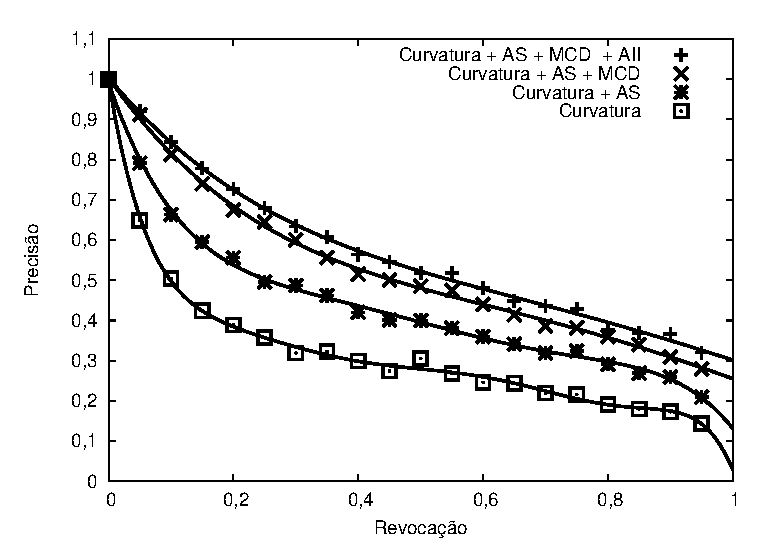
\includegraphics[width=0.75\textwidth]{graph1.eps}
\end{figure}


\section{\emph{Gap semântico}}
Uma questão importante nos sistemas \emph{CBIR} é que, embora os usuários busquem por imagens similares do ponto de vista semântico, o sistema provê os resultados com base na similaridade da informação extraída do conteúdo visual das imagens. A disparidade existente entre esses aspectos (semântica e conteúdo visual) é denominado de \emph{Gap} semântico.

Embora as imagens transmitam determinadas mensagens ao usuário, muito frequentemente os atributos extraídos das mesmas não conseguem representar e caracterizar essas mensagens. Diversos métodos para associar informação semântica aos atributos extraídos das imagens têm sido foco de pesquisa, como por exemplo solicitar que o usuário retro-alimente o sistema com o grau de relevância dos resultados obtidos (relevance feedback). 

\section{Base de imagens}

Um aspecto importante em \emph{CBIR} está ligado ao mecanismo de indexação empregado no acesso a informação contida na base de imagens. Em aplicações práticas, que requerem acesso a uma extensa base de dados, e aonde há interação dos usuários com o mecanismo de busca, o desempenho computacional no processo de indexação não pode ser negligenciado. Desta forma, armazenar vetores de características em um arquivo linear, com um registro para cada vetor, resulta na indexação sequencial destes elementos tornando essa abordagem inviável.

Todavia, mecanismos alternativos de indexação tradicionalmente encontrados na literatura, tais como \emph{k-d-b tree}, \emph{quad-tree} e \emph{R-tree} são considerados inadequados em \emph{CBIR} porque o desempenho destes se degrada substancialmente com o aumento da dimensionalidade dos dados. Ademais, para alcançar a eficiência computacional requerida sem degradar a qualidade das buscas, tais mecanismos devem levar em consideração a representação das características das imagens no processo de recuperação, ou seja, não só apenas \emph{como} indexar elementos na base de dados, mas também \emph{o que} indexar.

\end{comment}

% !TeX root = ../main.tex

\chapter{Resultados e Discussões \label{chap:resultados}}


Com o método de otimização proposto, realizamos experimentos de classificação e recuperação de formas pelo conteúdo, para dois descritores, com a base de folhas de plantas Flavia \cite{4458016},  que possui $1907$ imagens de folhas de $32$ espécies. A Figura \ref{fig:bases} ilustra imagens das folhas desta base. Cada exemplar ilustrado foi segmentado e colorido de acordo com a espécie ao qual pertence. Essa base de folhas é amplamente utilizada na validação de trabalhos de reconhecimento automático de espécies de plantas. 

\begin{figure}[!htb]
\caption{\label{fig:bases}Amostras de formas de folhas da base de imagens Flavia.}

\centering
\includegraphics[width=0.5\textwidth]{fig5.eps}
\end{figure}




\section{\emph{Classificação de formas e sua relação com  a função objetivo}}
Nos experimentos realizados para comparação dos algoritmos de otimização, avaliamos inicialmente aspectos  relacionados à  convergência dos algoritmos de otimização e a relação entre os resultados de classificação e as funções \ac{MAD}s obtidas por diferentes estratégias. Além disso investigamos o custo computacional dos mesmos. A Figura \ref{fig:converge} ilustra a convergência de cada um dos três algoritmos de otimização para $30$ repetições realizadas em um subconjunto da base de formas de folhas de plantas. Os resultados obtidos indicam que a otimização realizada pelo \ac{PSO} requereu um pequeno número de iterações para convergir a uma solução ótima, quando comparado aos algoritmos \ac{SA} e \ac{DE}. Uma vez que a convergência está relacionada com o número de iterações necessárias para se atingir uma solução ótima, um menor número de iterações implica em exploração deficiente do espaço de busca, ou seja, em convergência prematura \citeonline{Andries:2007}. Nestes casos, o método de otimização apresenta tendência de ficar preso a mínimos locais, encontrando assim soluções sub-ótimas para o problema. Por outro lado, a convergência mais lenta permite ao algoritmo explorar melhor o espaço de busca, aumentando portanto a chance deste convergir para um mínimo global, ou seja, uma solução ótima \citeonline{Andries:2007}.
 
Neste contexto, observa-se na Figura \ref{fig:converge}c que o \ac{PSO} encontrou soluções sub-ótimas com maior frequência, alcançando valores médios da função \ac{MAD}  igual a $0,805 \pm 0,006$.  Com relação aos algoritmos \ac{SA} e \ac{DE}, estes alcançaram os menores valores médios de \ac{MAD} : $0,795 \pm 0,006$ e $0,798 \pm 0,004$, respectivamente. Esses resultados demonstram que os algoritmos \ac{SA} e \ac{DE} foram mais eficazes que o \ac{PSO} em encontrar soluções ótimas. No entanto, o custo para alcançar tais soluções torna-se maior. A Seção \ref{sec:comp_cost} aborda com mais detalhes as questões relativas ao custo computacional dos algoritmos de otimização utilizados.

\begin{figure}[!htb]
\caption{\label{fig:converge} Convergência dos métodos de otimização para o problema de descrição de folhas de plantas: (a) \ac{SA}, (b) \ac{DE}, (c) \ac{PSO}. As curvas em vermelho destacam o valor médio da função \ac{MAD} para $30$ realizações de cada método (curvas em preto).} 

\includegraphics[width = \textwidth]{converge.jpg}
\end{figure}

A análise corrente tem como hipótese o fato de que as escalas otimizadas e o valor ótimo de \ac{MAD}, que estão inter-relacionadas, implicam em melhorias na taxa de acerto da classificação das espécies vegetais. A Tabela \ref{tab:leaves_supervised_results} exibe os diversos valores de \ac{MAD} e os correspondentes resultados obtidos nos experimentos de classificação para diferentes classificadores. Observa-se que os melhores resultados de classificação correspondem aos menores valores de \ac{MAD} obtidos através da metodologia de otimização de parâmetros. Os resultados de classificação para o descritor \ac{NMBE}, com as escalas ajustadas conforme sugerido por \citeonline{Costa:1997} ($\operatorname{\ac{NMBE}_{orig}}$), resultou em um desempenho intermediário quando comparado aos resultados para escalas otimizadas e escolhidas arbitrariamente. Os resultados mostram que o descritor \ac{NMBE} otimizado ($\operatorname{\ac{NMBE}_{opt}}$) melhorou o desempenho de todos os classificadores avaliados, uma vez que este alcançou as maiores taxas de Precisão e Revocação para os menores valores de \ac{MAD}, o que confirma a hipótese inicial.

Apesar do descritor \ac{NMBE} ter sido originalmente projetado para descrição de formas de neurônios, nesta tese o aplicamos com sucesso em caracterização de folhas de plantas, uma vez que a metodologia de otimização o ajustou ao problema em questão.
É importante ressaltar que os diferentes algoritmos de otimização, atingiram valores de \ac{MAD} distintos, e portanto conjuntos de escalas otimizadas distintos, os resultados de classificação corroboraram a hipótese e a conclusão anterior, pois tais conjuntos de escalas  permitiram que os descritores fossem capazes de capturar detalhes dos contornos das formas e as diferenciasse apropriadamente. Com isso, observamos que os algoritmos de otimização trazem vantagens à representação multiescala com impacto significativo na caracterização das folhas. 

\begin{table}[]
	\centering
	\caption{Valores de \ac{MAD} alcançados, pelos diferentes métodos empregados no ajuste das escalas do descritor \ac{NMBE}, para representação das folhas da base Flavia.}
	\label{tab:leaves_supervised_results}
	\begin{tabular}{ll}
		\toprule[1.5pt]
		Método de ajuste& \ac{MAD}\\
		\midrule
		\ac{SA}  & $0,762$\\
		\ac{DE}  & $0,783$\\
		\ac{PSO}&  $0,829$\\
		\citeonline{Cesar:1996}& $0,867$\\
		Empírico& $0,969$\\
		\bottomrule[1.5pt]
	\end{tabular}
\end{table}

\begin{figure}[!htb]
	\caption{\label{fig:leaves_fscore} Resultados de classificação das espécies vegetais da base de imagens Flavia para diferentes estratégias de escolha das escalas do descritor \ac{NMBE}.}
	\centering
	\includegraphics[width = 0.9\textwidth]{fscore.jpg}
\end{figure}


\begin{comment}
\begin{table}[]
\begin{minipage}{\textwidth}
\renewcommand\footnoterule{}
\caption{Valores de \ac{MAD} e resultados de classificação das espécies vegetais da base de imagens Flavia para diferentes estratégias de escolha das escalas do descritor \ac{NMBE}. }
\label{tab:leaves_supervised_results}
\resizebox{\textwidth}{!}{ 
\begin{tabular}{cccccccccc}
\toprule[1.5pt]
 & \multicolumn{8}{c}{Classifier} \\ \cmidrule(lr){2-9} 
 & \multicolumn{2}{c}{NB}  & \multicolumn{2}{c}{Knn (n = 5)}  & \multicolumn{2}{c}{LDA}  & \multicolumn{2}{c}{QDA} \\
\cmidrule(lr){2-3}  \cmidrule(lr){4-5} \cmidrule(lr){6-7}  \cmidrule(lr){8-9}
\ac{MAD} & Precision & Recall & Precision & Recall & Precision & Recall & Precision & Recall \\ \midrule
$0,762$\footnote{Using \ac{SA}}        & ${0,91 \pm 0,02}$   & ${0,89 \pm 0,02}$         & ${0,93 \pm 0,02}$          & ${0,92 \pm 0,02}$         & ${0,87  \pm 0,02}$          & ${0,85\pm 0,02}$         & ${0,95  \pm 0,01}$          & ${0,94  \pm 0,01}$         \\
$0,783$\footnote{Using \ac{DE}}        & $0,88 \pm 0,02$          & $0,87\pm0,02$         & $0,90\pm0,02$          & $0,88\pm0,02$         & $0,85\pm0,02$          & $0,83\pm0,03$         & $0,91\pm0,02$          & $0,90\pm0,02$         \\
$0,829$\footnote{Using \ac{PSO}}        & $0,86\pm0,03$          & $0,85\pm0,03$         & $0,89\pm0,03$          & $0,88\pm0,03$         & $0,84\pm0,03$         & $0,82\pm0,03$         & $0,91\pm0,02$          & $0,89\pm0,02$         \\
{$0,867$\footnote{Using scales proposed by \citeonline{Cesar:1996}}}          & $0,85\pm0,02$          & $0,84\pm0,02$         & $0,89\pm0,02$          & $0,88\pm0,02$         & $0,82\pm0,03$          & $0,81\pm0,03$         & $0,89\pm0,02$          & $0,88\pm0,02$         \\
{$0,969$\footnote{\label{note1}Random selection}}          & $0,81\pm0,03$          & $0,79\pm0,03$         & $0,87\pm0,02$          & $0,85\pm0,02$         & $0,77\pm0,03$          & $0,77\pm0,03$         & $0,87\pm0,03$          & $0,85\pm0,03$         \\
{$1,04$\footref{note1}}          & $0,69\pm0,03$          & $0,68\pm0,03$         & $0,83\pm0,03$          & $0,82\pm0,03$         & $0,74\pm0,03$          & $0,73\pm0,03$         & $0,81\pm0,03$          & $0,79\pm0,03$         \\
\bottomrule[1.5pt]
\end{tabular}}
\end{minipage}
\end{table}
\end{comment}
  
Os resultados da Tabela \ref{tab:leaves_supervised_results} confirmam que os classificadores que utilizaram descritores gerados a partir de escalas selecionadas arbitrariamente não tiveram desempenho satisfatório, pois alcançaram os menores valores de Precisão e Revocação e os maiores valores da função \ac{MAD}. Portanto, escalas aleatórias levam a uma representação multiescala menos sensível a variações de características das folhas, consequentemente, mais erros de classificação. 

\section{\emph{Análise exploratória visual de agrupamentos}}

Nesta seção utilizamos técnicas de visualização de dados multidimensionais, como \ac{MDS} e matriz-U, para observar os resultados dos descritores multiescala \ac{NMBE} e \ac{DFM}. O uso dessas técnicas suportam a análise do comportamento dos descritores a partir de suas relações com os agrupamentos observados em um espaço bidimensional. 

%As três imagens na Figura \ref{fig:nuvem_pca} representam projeções bidimensionais das duas primeiras componentes principais (mais relevantes) dos vetores de características obtidos a partir dos descritores \ac{NMBE} e \ac{DFM} transformados através da \emph{PCA}, assim como a combinação de ambos. Os números anotados dentro dos gráficos indicam a acurácia média por classe. Visualmente as projeções das duas componentes indicam a complexidade do problema da análise de formas, a dimensionalidade do problema e a dificuldade em projetar descritores e ajustar seus parâmetros de modo que descrevam as mais diversas nuances de formas de bases de uso geral (Kimia-99, Kimia-216, MPEG7 CE-Shape-1) e aplicadas (Flavia). Observa-se que a qualidade dos agrupamentos em geral não é boa para todas as classes, quando se aplica \ac{NMBE} e \ac{DFM}, entretanto a combinação de ambos os descritores elevou a qualidade da discriminação das formas e da recuperação das mesmas.  

%\begin{figure}[t]
%  \caption{\label{fig:nuvem_pca} Imagens das projeções das duas primeiras componentes principais, obtidas através de PCA, dos vetores de características transformados para os descritores \ac{NMBE} e  \ac{DFM} individualmente e combinados.}
%  \centering
%  \includegraphics[width=0.75\textwidth]{nuvem_pca.eps}
%\end{figure}

\begin{figure}[t]
 \caption{\label{fig:nmbe_dfm_99} Resultados dos descritores \ac{NMBE} e \ac{DFM} para a base Kimia-99. (a) Matriz-U obtida com o descritor \ac{NMBE} e respectiva \textit{Silhouette} média por classe. (b) Matriz-U obtida com o descritor \ac{DFM} e respectiva \textit{Silhouette} média por classe.}
  \centering
  \includegraphics[width=\textwidth]{nmbe_dfm_99.jpg}
\end{figure}

\begin{figure}[t]
 \caption{\label{fig:nmbe_dfm_216} Resultados dos descritores \ac{NMBE} e \ac{DFM} para a base Kimia-216. (a) Matriz-U obtida com o descritor \ac{NMBE} e respectiva \textit{Silhouette} média por classe. (b) Matriz-U obtida com o descritor \ac{DFM} e respectiva \textit{Silhouette} média por classe.}
  \centering
  \includegraphics[width=\textwidth]{nmbe_dfm_216.jpg}
\end{figure}

Para ilustrar o poder discriminativo dos descritores de forma multiescala \ac{NMBE} e \ac{DFM}, bem como mostrar a relação existente entre a medida de avaliação quantitativa da qualidade dos agrupamentos, \emph{silhouette}, e a representação qualitativa obtida através da matriz U, foram realizadas as extrações de características das formas das bases Kimia-99 e Kimia-216 com os referidos descritores. Os resultados estão expostos nas Figuras \ref{fig:nmbe_dfm_99} e \ref{fig:nmbe_dfm_216}. 

Em ambas as figuras, observa-se que as formas correspondentes às classes com  \emph{silhouette} média positiva são visualizadas na matriz-U mantendo forte relação de vizinhança entre si, enquanto que formas correspondentes às classes cuja \emph{silhouette} média é negativa encontram-se dispersas nessas matrizes. Isso denota a inabilidade da descrição  em representá-las adequadamente.

Assim, os descritores conseguem capturar características tanto globais como locais, uma vez que classes de formas com características globais semelhantes, como por exemplo as formas alongadas do canto superior esquerdo da Figura \ref{fig:nmbe_dfm_216}a, estabelecem uma relação de vizinhança entre si. Apesar disso, formas alongadas de classes distintas não se misturam, o que é um indicativo de que o descritor foi capaz também de representar características locais discriminativas que permitem a separação entre as classes.

Existem no entanto casos, em que ambos os descritores não foram capazes de discriminar formas com características globais semelhantes, como é o caso das classes de formas de elefantes e camelos na Figura \ref{fig:nmbe_dfm_216}. Na matriz-U, estas formas aparecem agrupadas como se pertencessem a uma mesma classe e consequentemente, com valores de \emph{silhouette} média significativamente menores em relação às formas que foram discriminadas corretamente pelos descritores.

A Figura \ref{fig:MatrizU_leaves_256}a mostra a matriz-U obtida para as formas de folhas de plantas da base Flavia representadas pelo descritor \ac{NMBE} otimizado e a Figura \ref{fig:MatrizU_leaves_256}b, pelo descritor \ac{NMBE} não otimizado. A análise exploratória visual dos agrupamentos produzidos pela descrição \ac{NMBE} indica que a descrição otimizada melhora a organização dos agrupamentos. Essa evidência então confirma que a função objetivo \ac{MAD} é adequada para guiar o processo de otimização desse descritor. A visualização das formas nas matrizes-U da Figura \ref{fig:MatrizU_leaves_256}  aponta diferenças entre os dois arranjos promovidos pelos referidos descritores. A cada posição ou elemento da matriz, os valores numéricos foram substituídos pela imagem das folhas correspondentes, estando as cores das folhas em correspondência com o rótulo das classes exibidas na Figura \ref{fig:bases}. Nessas matrizes-U,  estão representadas as $1907$ formas de folhas da base Flavia, sendo cada folha representada por sua descrição multiescala.

Os gráficos representativos da \emph{silhouette} média nas Figuras \ref{fig:MatrizU_leaves_256}a  e \ref{fig:MatrizU_leaves_256}b demonstram que as classes das folhas bem caracterizadas e, portanto, agrupadas adequadamente são as que apresentam valores de \emph{silhouette} média positivos. Por outro lado, as classes de folhas cujo descritor não foi capaz de caracterizar e agrupar adequadamente são as que apresentaram valores negativos de \emph{silhouette} média. Comparando estes resultados, observa-se que na Figura \ref{fig:MatrizU_leaves_256}a há expressiva redução dos valores negativos de \emph{silhouette} média quando se utiliza o descritor $\operatorname{\ac{NMBE}_{opt}}$. 

\begin{figure}[t]

\caption{\label{fig:MatrizU_leaves_256} Matrizes-U e a \emph{silhouette} média para as descrições das folhas da base Flavia com o descritor \ac{NMBE} (a) optimizado e (b) não otimizado.}
\centering
\includegraphics[width=\textwidth]{Umat_leaves.jpg}

\end{figure}

O quadrado preto inserido na Figura \ref{fig:MatrizU_leaves_256} destaca o desempenho do descritor otimizado em termos de melhoria no arranjo das formas na matriz-U. É possível ainda observar quão bem o descritor otimizado mapeou as folhas em grupos de acordo com as respectivas classes rotuladas das mesmas.  Além do mais, o resultado com as escalas otimizadas melhorou significativamente a \emph{silhouette} média por classe para quase todas as classes de folhas da base. Por outro lado, a região interna ao quadrado preto na Figura \ref{fig:MatrizU_leaves_256}b destaca que o descritor não otimizado não foi capaz de mapear satisfatoriamente as formas de  folhas em suas classes correspondentes. Deduzimos que essa melhoria se deve ao fato de que as escalas otimizadas dos descritores são mais sensíveis a variações intrínsecas das formas, ou seja, incorporam nuances presentes nos seus contornos, os quais os métodos tradicionais não fazem adequadamente. Ademais, o ajuste automático das escalas é de fato uma tarefa alternativa para o ajuste arbitrário ou empírico, sendo que esta última não é uma tarefa simples e está sujeita à fadiga e subjetividade do realizador da mesma.


As Figuras \ref{fig:MatrizU_leaves_II}a, \ref{fig:MatrizU_leaves_II}b and \ref{fig:MatrizU_leaves_II}c exibem as matrizes-U correspondentes aos valores \ac{MAD} dos experimentos na base Flavia utilizando os algoritmos de otimização \ac{SA}, \ac{DE} e \ac{PSO}, respectivamente. Um aspecto interessante a examinar é o fato dos três algoritmos apresentarem diferentes soluções, ou valores de \ac{MAD}. Estas soluções resultaram em diferentes arranjos de folhas e consequentemente diferentes relações entre as estruturas de vizinhança dos grupos ou classes.
Por exemplo, a dispersão geral dos elementos nas Figuras \ref{fig:MatrizU_leaves_II}a e \ref{fig:MatrizU_leaves_II}b tende a ser muito semelhante uma vez que seus respectivos valores da função objetivo minimizada são bem próximos em magnitude. Ao mesmo tempo, concluímos que o resultado que corresponde ao mais elevado valor de \ac{MAD} ($0,829$) exibe uma dispersão particularmente elevada no centro da matriz-U (Figura \ref{fig:MatrizU_leaves_II}c). Este é um detalhe que reforça a observação anterior de que o \ac{PSO} convergiu para um mínimo local. 
Estes achados apontam para a importante conclusão de que quanto menor o valor de \ac{MAD}, melhor o arranjo dos grupos ou do agrupamento, e consequentemente a qualidade do agrupamento. Por isso, afirmamos que a qualidade dos grupos e o valor de \ac{MAD} são negativamente correlacionados. Nossa análise ainda considera que devam existir outras soluções no espaço de busca, além da solução mínima, que sejam adequadas ao problema em estudo.

\begin{figure}[h!] \caption{\label{fig:MatrizU_leaves_II}Matrizes-U e valores \ac{MAD}s obtidos para a base de imagens Flavia por uso da \ac{NMBE} otimizada pelos algoritmos (a) \ac{SA}, (b) \ac{DE}, (c) \ac{PSO}.}
\centering
\includegraphics[width=\textwidth]{Umat_SA_DE_PSO_v2.jpg}
\end{figure}

A Figura \ref{MDS:Leaves} ilustra as projeções \ac{MDS} para três valores distintos de \ac{MAD}. Na Figura \ref{MDS:Leaves}a,  temos o arranjo dos agrupamentos após a convergência do algoritmo de otimização \ac{SA}, ou seja, para o descritor cujos parâmetros otimizados correspondem ao mínimo valor da função \ac{MAD} encontrado nas otimizações. Analisando essas projeções, observa-se que a minimização da função objetivo resultou em agrupamentos de folhas com maior coesão intra classe e maior separação entre classes. A análise visual das três regiões detalhadas  nessa imagem indica mais claramente que o descritor \ac{NMBE} otimizado melhorou a representação das formas de folhas em comparação aos resultados das Figuras \ref{MDS:Leaves}b e \ref{MDS:Leaves}c. Ademais, os valores do coeficiente $R^2$ próximos de $1,0$ indicam que a representação no espaço bi-dimensional preservou a relação de distâncias entre as amostras no espaço de alta dimensão.

\begin{figure}[t]
 \caption{\label{MDS:Leaves} Projeções \ac{MDS} dos descritores \ac{NMBE} para formas da base de folhas Flavia. (a) Descritor \ac{NMBE} otimizado pelo algoritmo \ac{SA} com valor de função $\ac{MAD} = 0,762$ (b) Descritor \ac{NMBE} não otimizado com valor de função $\ac{MAD} =0,969$ and (c) Descritor \ac{NMBE} não otimizado com valor de função $\ac{MAD} = 1,044$.}

\centering
\includegraphics[width=\textwidth]{MDS_Leaves.jpg}
\end{figure}

\section{Recuperação de imagens baseada em conteúdo}

O descritor \ac{IDSC} \cite{Ling:2007:SCU:1191552.1191806} foi otimizado para fins de comparação com o descritor multiescala. Desenvolvido para aplicações de recuperação de formas, o \ac{IDSC} utiliza algoritmos de programação dinâmica, tal como o \ac{DTW} \cite{PalazonGonzalez2012978}, para melhorar a precisão da avaliação de similaridade entre formas. Assim sendo, subsituimos a norma $L_2$ pelo algoritmo \ac{DTW} no cálculo da medida \emph{silhouette}, uma vez que esta última é requerida para a avaliação da função objetivo \ac{MAD} na Equação \ref{eq:mad}. 

A Figura \ref{fig1Ooptimization_graph}a exibe gráficos que permitem a comparação dos resultados dos experimentos realizados para as versões otimizadas ($\operatorname{\ac{NMBE}_{opt}}$, $\operatorname{\ac{IDSC}_{opt}}$)
 e não otimizadas ($\operatorname{\ac{NMBE}}$, $\operatorname{\ac{IDSC}}$) de ambos descritores. Os gráficos mostram que o ajuste dos parâmetros dos descritores pelo método de otimização melhorou o resultado (taxa) de recuperação de folhas consideravelmente. Observamos ainda que o descritor $\operatorname{\ac{IDSC}_{opt}}$ superou ambos os descritores $\operatorname{\ac{NMBE}_{opt}}$ e \ac{NMBE} não otimizado com relação à taxa de recuperação. Logo, podemos afirmar que a otimização de parâmetros melhorou a capacidade de discriminação do  $\operatorname{\ac{IDSC}_{opt}}$, incorporando ao descritor um mecanismo de extração de informações relevantes de detalhes intrínsecos das formas das folhas. Por outro lado, observamos que o desempenho do \ac{IDSC} não otimizado foi inferior ao do \ac{NMBE} não otimizado. 

As Figuras \ref{fig1Ooptimization_graph}b e \ref{fig1Ooptimization_graph}c ilustram resultados obtidos de recuperação de dois exemplares da base de imagens de folhas para experimentos realizados com os descritores \ac{NMBE} não otimizado e $\operatorname{\ac{NMBE}_{opt}}$,  \ac{IDSC} não otimizado com parâmetros ajustados conforme recomendado em \cite{wang2015march} e $\operatorname{\ac{IDSC}_{opt}}$. Observa-se na Figura \ref{fig1Ooptimization_graph}b que o descritor \ac{NMBE} não otimizado falhou parcialmente na recuperação das formas, enquanto a versão otimizada ($\operatorname{\ac{NMBE}_{opt}}$) com sucesso recuperou todas as formas. O mesmo comentário se aplica ao descritor $\operatorname{\ac{IDSC}_{opt}}$, cujos resultados mostram o sucesso da recuperação. Ainda na Figura \ref{fig1Ooptimization_graph}c, o descritor \ac{IDSC} não otimizado não foi capaz de recuperar as amostras corretamente.

\begin{figure}[]
\caption{Experimentos realizados com formas da base de imagens de folhas Flavia (a) taxa de recuperação  obtida com os descritores \ac{NMBE} e \ac{IDSC} originais e suas versões otimizadas, (b) e (c) recuperação de duas amostras de folhas utilizando os descritores \ac{NMBE} e \ac{IDSC} otimizados e não otimizados, respectivamente.\label{fig1Ooptimization_graph}}
\includegraphics[width=\textwidth]{res_cbir.jpg}
\end{figure}

\begin{comment}
\begin{figure}[t!]
\begin{subfigure}{0.55\textwidth}
\includegraphics[width=\textwidth]{fig10a.eps}
\caption{Retrieval rates. \label{fig1Ooptimization_graph}}
\end{subfigure}
\hspace*{\fill}
\begin{minipage}{0.45\textwidth}
\begin{subfigure}{\textwidth}
\includegraphics[width=\textwidth]{fig10b.eps}
\caption{Retrieval results with \ac{NMBE}.} \label{subfig:upper-right}

\end{subfigure}

\vspace*{0.60cm}
\begin{subfigure}{\textwidth}
\includegraphics[width=\textwidth]{fig10c.eps}
\caption{Retrieval results with \ac{IDSC}.\label{subfig:lower-right}}
\end{subfigure}
\end{minipage}

\caption{\label{figfig1Optmization-IDSC} Experiments conducted on Flavia leaf data set (a) retrieval rate by using both \ac{NMBE} and \ac{IDSC} and their optimized counterparts, (b) and (c) two leaf shape retrieval examples by using the non-optimized and optimized \ac{NMBE} and \ac{IDSC} descriptors, respectively.} 
\end{figure}
\end{comment}

A Tabela \ref{table_bull_eyes_leaves} apresenta o resultado da avaliação de desempenho dos descritores $\operatorname{\ac{NMBE}_{opt}}$ e \ac{NMBE} não otimizado com escalas ajustadas conforme recomendado em \cite{Cesar:1996},  $\operatorname{\ac{IDSC}_{opt}}$ e o \ac{IDSC} não otimizado. Esses resultados mostram que a taxa de recuperação para ambos os descritores otimizados superou os resultados dos pares correspondentes não otimizados. A melhoria significativa observada nas medidas Bulls-eye reforça a hipótese de que a metodologia de otimização proposta é adequada para ajuste dos descritores em aplicações de recuperação e análise de formas de folhas.

\begin{table}[h!]
\centering
\caption{Taxa Bulls-eye para a base de imagens Flavia.}
\label{table_bull_eyes_leaves}
  \begin{tabular}{cccccccc}
  \toprule[1.5pt]
 $\operatorname{\ac{NMBE}}$ & $\operatorname{\ac{NMBE}_{opt}}$ & \ac{IDSC}    & $\operatorname{\ac{IDSC}_{opt}}$\\ \midrule
     63,86 \%  & 71,16 \%  & 53,38\%    & 77,50\%       \\
  \bottomrule[1.5pt]
  \end{tabular}
\end{table}

\section{Custo computacional da otimização \label{sec:comp_cost}}


 Nesta tese,  avaliamos a complexidade computacional dos três algoritmos de otimização como exibe a Tabela \ref{tbl:complexity}.  Os algoritmos \ac{SA} e \ac{PSO} apresentam complexidades similares e estas dependem do número de iterações para convergir ($N_{iter}$), do tamanho da população  ($N_{pop}$) e do parâmetro $P$.  Por outro lado, o algoritmo \ac{DE} demanda maior complexidade, pois depende da dimensão ($D$) do problema a ser otimizado, do tamanho da população ($N_{pop}$) e do número de interações ($N_{iter}$).

\begin{table}[h!]
\centering
\caption{Complexidade computacional dos métodos de otimização.}
\label{tbl:complexity}
  \begin{tabular}{llr}
  \toprule[1.5pt]
 Método & Complexidade& Custo\\
 \midrule
   \ac{SA}  & $O(P.N_{iter}.\log{N_{iter}})$ & $7.431$    \\
   \ac{DE}  & $O(N_{pop}.N_{iter}.D)$ & $19.500$  \\
   \ac{PSO}&  $O(N_{pop}.N_{iter}.\log{N_{iter}})$ & $1.107$\\
  \bottomrule[1.5pt]
  \end{tabular}
\end{table}

Para fins de comparação dos métodos de otimização, sob o aspecto de custo computacional, assumimos como custo dos algoritmos o número de vezes que a função objetivo é demandada ao longo do processo de otimização. Considerando para cada método de otimização o ajuste de parâmetros adotado, bem como a complexidade computacional correspondente, os custos computacionais calculados para os algoritmos \ac{SA}, \ac{DE} e \ac{PSO} resultaram em $7.431$, $19.500$ e $1.107$, respectivamente. 

Vale destacar que existe um compromisso entre o custo computacional e a qualidade da solução obtida. Assim sendo a redução do número de amostras de formas, da resolução das imagens e do tamanho da população dos métodos ($N_{pop}$) ameniza o custo computacional, porém estas reduções degradam a qualidade do resultado da otimização. Ademais, o uso de processamento paralelo pode contribuir para a redução do custo computacional, sem degradar a qualidade da solução ótima, entretanto o paralelismo adiciona complexidade aos algoritmos de otimização. 



\begin{comment}
\begin{figure}
 \caption{\label{fig:edif99} (a) Matriz-U para as formas da base Kimia99 representadas com o descritor entropia multiescala. (b) Silhouette média por classe aferida a partir do descritor}
  \centering
  \includegraphics[width=\textwidth]{ediferencial99.png}
\end{figure}

\begin{figure}
 \caption{\label{fig:edif216} (a) Matriz-U para as formas da base Kimia216 representadas com o descritor entropia multiescala. (b) Silhouette média por classe aferida a partir do descritor}
  \centering
  \includegraphics[width=\textwidth]{ediferencial216.png}
\end{figure}

\begin{figure}
 \caption{\label{fig:edis99} (a) Matriz-U para as formas da base Kimia99 representadas com o descritor entropia multiescala. (b) Silhouette média por classe aferida a partir do descritor}
  \centering
  \includegraphics[width=\textwidth]{ediscreta99.png}
\end{figure}

\begin{figure}
 \caption{\label{fig:edis216} (a) Matriz-U para as formas da base Kimia216 representadas com o descritor entropia multiescala. (b) Silhouette média por classe aferida a partir do descritor}
  \centering
  \includegraphics[width=\textwidth]{ediscreta216.png}
\end{figure}

\subsection{\ac{NMBE} e \ac{DFM}}
Os experimentos de avaliação de desempenho dos descritores produziram como saída as matrizes-U que estão apresentadas na Figuras \ref{fig:nmbe_som_map}, \ref{fig:mfd_som_map} e  \ref{fig:som_kimia_216}. Nas Figuras \ref{fig:nmbe_som_map} e \ref{fig:mfd_som_map}, as regiões delimitadas com linhas tracejadas correspondem as classes de formas com os maiores valores médios da medida Silhouette (Figuras \ref{fig:silhouette}a e \ref{fig:silhouette}b). Nesses casos pode-se deduzir que ambos os descritores foram capazes de caracterizar corretamente estas classes de formas.

Já os grupos delimitados com linhas contínuas referem-se às classes de formas com os menores valores de Silhouette média. De fato, as formas dessas classes aparecem nas matrizes-U dispersas em sub-grupos, que é um indicativo que ambos os descritores falharam em caracterizá-las adequadamente.
  
As Figuras \ref{fig:dude_tool_mfd} e \ref{fig:dude_tool_nmbe} mostram objetos das classes de formas de humanos e ferramentas. Ambos os descritores foram capazes de discriminar os objetos das referidas classes, como evidenciado nos gráficos apresentados. As matrizes-U (Figuras \ref{fig:nmbe_som_map} e \ref{fig:mfd_som_map}) também confirmam esse resultado exibindo, para essas classes de formas, homogeneidade intra-classe e separabilidade inter-classes. Logo, concluímos que estes descritores são efetivos em representar formas para o reconhecimento de padrões em aplicações \ac{CBIR}.

Também evidenciamos nas Figuras \ref{fig:mfd_som_map} e \ref{fig:nmbe_som_map} que o descritor \ac{DFM} apresentou maior dispersão inter-classe para as formas de humanos que o descritor \ac{NMBE}. Essa observação é consistente com os resultados obtidos através da medida \emph{Silhouete}, aonde o valor dessa medida para formas humanas descritas com a \ac{DFM} é menor do que o valor para essas mesmas formas descritas com a \ac{NMBE}.

Ademais, os sinais em linhas tracejadas vermelhas e em linhas contínuas azuis, apresentados nas Figuras \ref{fig:dude_tool_mfd} e \ref{fig:dude_tool_nmbe}, mostram que o descritor \ac{NMBE} é mais robusto a diferenças intra-classe que o descritor \ac{DFM}. Nesses gráficos, as formas pertencentes a mesma classe que o descritor representa seguindo um mesmo padrão apresentam-se próximas umas das outras na matriz-U, enquanto as formas que o descritor representa divergindo do padrão são mapeadas na matriz-U distantes dos grupo correspondente. Exemplos desta última condição são as formas humanas rotuladas como $2$ e $4$ nas Figuras \ref{fig:dude_tool_mfd} e \ref{fig:dude_tool_nmbe}.


Furthermore, there is a larger variation among tools descriptions in the graphs of  the figure \ref{fig:descritores}a than the  variations observed in the graphs of the figure \ref{fig:descritores}b. Coherently, the corresponding shapes appears in the U-matrix more dispersed  for the \emph{MFD} description than for the \ac{NMBE} description.

\begin{figure}[h!]
  \caption{\label{fig:nmbe_som_map} Matriz-U para as formas da base Kimia99 representadas com o descritor Energia de dobramento multiescala.}
  \centering
  \includegraphics[width=0.5\textwidth]{nmbe_som_map_v4.eps}
\end{figure}

\begin{figure}[h!]
  \caption{\label{fig:mfd_som_map} Matriz-U para as formas da base Kimia99 representadas com o descritor Dimensão fractal multiescala.}
  \centering
  \includegraphics[width=0.5\textwidth]{mfd_som_map_v3.eps}
\end{figure}
  
\begin{figure}[h!]  \caption{\label{fig:som_kimia_216} Para o descritor energia de dobramento multiescala e a base Kimia-216: (a) Matriz-U. (b) Alguns resultados de recuperação de formas pelo conteúdo.}
  \centering
  \includegraphics[width=0.5\textwidth]{retr_som_kimia216_v2.png}
\end{figure}

Já a Figura \ref{fig:som_kimia_216}a apresenta os resultados da visualização das formas da base Kimia-216 representadas através do descritor \ac{NMBE}. No canto inferior direito desta figura observamos que o descritor confunde formas dos elefantes com as dos camelos. Essa confusão aparece também no experimento de recuperação de formas pelo conteúdo (Figura \ref{fig:som_kimia_216}b), em que uma dentre as formas dos elefantes é utilizada como protótipo para se recuperar as onze formas mais similares ao protótipo na referida base.

Analogamente, no canto superior esquerdo da Figura \ref{fig:som_kimia_216}a, há confusão entre os agrupamentos das formas das faces e dos corações, bem como a presença duma forma de garfo. Na segunda linha da Figura \ref{fig:som_kimia_216}b observamos a presença dessas formas indesejáveis no experimento de recuperação de formas quando uma forma de face é apresentada como protótipo. 

Os demais resultados de recuperação de formas, apresentados na Figura \ref{fig:som_kimia_216}b, também estão coerentes com as observações da matriz-U. Nessa última podemos observar que o grupo das formas das arraias são mapeadas vizinhas aos grupos das formas dos cálices e dos pássaros, o que resulta no aparecimento das formas dessas últimas classes quando se realiza a recuperação de arraias. 

Outro aspecto importante de ser observado é que  grupos de formas com similaridades grosseiras encontram-se mapeados próximos uns dos outros na matriz-U. Formas alongadas, por exemplo, estão organizadas na parte inferior esquerda da Figura \ref{fig:som_kimia_216}a, enquanto formas arredondadas encontram-se na parte superior. Outros exemplos incluem os seguintes grupos: chaves e crianças (esquerda da figura), carros e tijolos, tartarugas e pássaros, cálices e sepulturas. 

\begin{figure}[h!]
  \caption{\label{fig:silhouette} Silhouette média por classe aferida, com a base Kimia-99, para os descritores (a) Dimensão fractal multiescala; (b) Energia de dobramento multiescala.}
  \centering
  \includegraphics[width=0.5\textwidth]{resultado_silhouette.eps}
\end{figure}

\begin{figure}[h!]
  \caption{\label{fig:dude_tool_mfd}   Vetores de características calculados para amostras das formas de humanos e de ferramentas com o descritor dimensão fractal multiescala.}
  \centering
  \includegraphics[width=0.75\textwidth]{dude_tool_mfd_v6.eps}
\end{figure}

\begin{figure}[h!]
  \caption{\label{fig:dude_tool_nmbe} Vetores de características calculados para amostras das formas de humanos e de ferramentes com o descritor energia de dobramento multiescala.}
  \centering
  \includegraphics[width=0.75\textwidth]{dude_tool_nmbe_v6.eps}
\end{figure}

\subsection{Entropia diferencial da curvatura multiescala}

A visualização de dados obtida para características extraídas com o descritor entropia diferencial da curvatura multiescala, para a base Kimia-99, está apresentada na Figura \ref{fig:edif99}a. Nesta figura observamos a Matriz-U, em tons de cinza, sobreposta às figuras das formas nas posições mapeadas pela rede SOM.

As células escuras formam contornos que delimitam fronteiras existentes entre agrupamentos de formas, pois estas células indicam a existência duma relação de separação entre as formas em suas vizinhanças. Já as células em linhas claras indicam maior proximidade entre as formas e suas vizinhanças.

Podemos inferir que o descritor representou adequadamente as formas das classes de humanos, arraias, peixes, ferramentas e coelhos. Isso porque, nestes casos, o descritor apresentou uma representação compacta, agrupando próximas as formas de uma mesma classe, e propiciando separabilidade entre os agrupamentos estabelecidos. A medida Silhouette média por classe, apresentada na Figura \ref{fig:edif99}b, corrobora nossas observações, pois as referidas classes são as que apresentam os valores de Silhouette média mais positivos e com pequeno desvio padrão.  

Por outro lado, o descritor falhou em representar as formas das classes de animais quadrúpedes, aviões e extra terrestres. Isso porque, nesses casos, não se consegue identificar na matriz-U fronteiras claras que estabeleçam um único agrupamento das formas de uma mesma classe. Em outras palavras, formas dessas classes encontram-se separadas umas das outras ou dispersas em sub-grupos delimitados por pequenas fronteiras. Esses casos são os que apresentam a medida Silhouette média por classe com os menores valores e os maiores desvios padrão. 

Já na Figura \ref{fig:edif216}a temos a visualização da matriz-U para as características extraídas das formas da base Kimia-216. Nesta observamos, bem delimitados por linhas escuras, diversos agrupamentos  representados corretamente pelo descritor. Dentre esses, destacamos os agrupamentos cujas fronteiras de separação intra-classe são de baixo contraste e cujas fronteiras de separação inter-classe são bem contrastadas (faces, garfos, sepulturas, cálices e crianças). Esses são os  agrupamentos que apresentaram os maiores valores de \emph{Silhouette} média na Figura \ref{fig:edif216}b, o que é um resultado esperado, uma vez que o descritor representou as formas desses grupos de forma compacta e em agrupamentos bem separados.

\begin{figure}
\caption{\label{fig:edif_som_map} Matriz-U para as formas da base Kimia99 representadas com o descritor Entropia diferencial da curvatura multiescala.}
  \centering
  \includegraphics[width=\textwidth]{ediferencial_N5_formas.png}
 \end{figure}

\begin{figure}
\caption{\label{fig:silhouette_ediferencial} Silhouette média por classe aferida, com a base Kimia-99, para o descritor entropia diferencial da curvatura multiescala.}
  \centering
  \includegraphics[width=0.75\textwidth]{ediferencial_silhouette_N5.png}
\end{figure}

\begin{figure}[h!]
  \caption{\label{fig:som_nmbe} Visualização dos dados obtida com o mapa auto-organizável de Kohonen para a descrição \ac{NMBE}.}
  \centering
  \includegraphics[width=0.5\textwidth]{mapa_som_descritor_nmbe.png}
\end{figure}

\begin{figure}[h!]
  \caption{\label{fig:som_dfm} Visualização dos dados obtida com o mapa auto-organizável de Kohonen para a descrição \ac{NMBE}.}
  \centering
  \includegraphics[width=0.5\textwidth]{mapa_som_descritor_dfm.png}
\end{figure}

\section{Recuperação de imagens pelo conteúdo}

\begin{table*}
\centering
\caption{\label{tab:KimiaChernoff} Total de acertos por classe e por posição, nos experimentos \ac{CBIR}, com a distância de Chernoff.}
\begin{tabular}{l| r r r r r r r r r r r}
\hline
&\multicolumn{11}{l}{nth nearest match} \\
\cline{2-12}
Classe&1&2&3&4&5&6&7&8&9&10&11 \\
 \hline
Peixes&11&11&11&11&9&5&8&3&7&5&5\\
Coelhos&11&11&11&11&11&11&11&11&11&11&7\\ 
Aviões&11&10&8&8&7&7&7&5&2&1&1\\
ETs&11&11&11&11&11&11&11&11&8&7&5\\
Ferramentas&11&8&7&10&3&9&9&5&7&9&9\\
Mãos&11&11&11&11&11&11&11&11&11&9&7\\
humanos&11&11&11&11&11&11&11&11&11&11&11\\
Quadrupedes&11&11&9&8&8&7&8&3&5&8&4\\
Arraias&11&11&11&11&11&11&11&10&11&9&7\\
\hline
Total&99&95&90&92&82&83&87&70&73&70&56\\
\hline
\end{tabular}
\end{table*}

\begin{table*}
\centering
\caption{\label{tab:KimiaChi-square} Total de acertos por classe e por posição, nos experimentos \ac{CBIR}, com a distância de Chi-square.}
\begin{tabular}{l| r r r r r r r r r r r}
\hline
&\multicolumn{11}{l}{nth nearest match} \\
\cline{2-12}
Classe&1&2&3&4&5&6&7&8&9&10&11 \\
 \hline
Peixes&11&11&11&10&10&8&7&9&4&4&3\\
Coelhos&11&10&10&10&10&10&10&10&10&8&1\\ 
Aviões&11&11&11&9&9&9&8&5&2&2&2\\
ETs&11&11&11&10&11&10&11&10&10&8&7\\
Ferramentas&11&11&11&11&11&11&11&11&10&11& 11\\
Mãos&11&11&11&11&11&11&11&11&11&11&9\\
humanos&11&11&11&11&11&11&11&11&11&11&11\\
Quadrupedes&11&11&6&9&8&7&7&5&7&7&4\\
Arraias&11&11&11&11&11&11&11&10&11&11&10\\
\hline
Total&99&98&93&92&92&88&87&82&76&73&58\\
\hline
\end{tabular}
\end{table*}

\begin{table*}
\centering
\caption{\label{tab:KimiaHellinger} Total de acertos por classe e por posição, nos experimentos \ac{CBIR}, com a distância de Hellinger.}
\begin{tabular}{l| r r r r r r r r r r r}
\hline
&\multicolumn{11}{l}{nth nearest match} \\
\cline{2-12}
Classe&1&2&3&4&5&6&7&8&9&10&11 \\
 \hline
Peixes&11&11&11&10&10&9&5&8&8&2&2\\
Coelhos&11&11&11&11&11&10&10&10&11&8&2\\ 
Aviões&11&11&11&10&9&11&9&8&1&1&0\\
ETs&11&11&11&11&10&11&10&11&11&7&4\\
Ferramentas&11&11&11&11&11&11&11&10&11&11& 10\\
Mãos&11&11&11&11&11&11&11&11&11&11&8\\
humanos&11&11&11&11&11&11&11&11&11&11&11\\
Quadrupedes&11&11&7&9&6&6&5&7&9&5&4\\
Arraias&11&11&11&11&11&11&11&11&11&10&9\\
\hline
Total&99&99&95&95&90&91&83&87&84&66&50\\
\hline
\end{tabular}
\end{table*}

\begin{table*}
\centering
\caption{\label{tab:KimiaJensen-Shannon} Total de acertos por classe e por posição, nos experimentos \ac{CBIR}, com a distância Jensen-Shannon.}
\begin{tabular}{l| r r r r r r r r r r r}
\hline
&\multicolumn{11}{l}{nth nearest match} \\
\cline{2-12}
Classe&1&2&3&4&5&6&7&8&9&10&11 \\
 \hline
Peixes&11&11&11&10&10&8&7&7&7&4&1\\
Coelhos&11&10&10&10&10&10&10&10&9&8&2\\ 
Aviões&11&11&10&10&9&8&8&6&3&1&1\\
ETs&11&11&11&10&11&10&10&11&9&8&5\\
Ferramentas&11&11&11&11&11&11&11&11&10&11& 11\\
Mãos&11&11&11&11&11&11&11&11&11&11&9\\
humanos&11&11&11&11&11&11&11&11&11&11&11\\
Quadrupedes&11&11&7&8&8&5&3&8&8&7&4\\
Arraias&11&11&11&11&11&11&11&11&10&11&10\\
\hline
Total&99&98&93&92&92&85&82&86&78&72&54\\
\hline
\end{tabular}
\end{table*}

\begin{table*}
\centering
\caption{\label{tab:KimiaPatrick-Fisher} Total de acertos por classe e por posição, nos experimentos \ac{CBIR}, com a distância Patrick-Fisher.}
\begin{tabular}{l| r r r r r r r r r r r}
\hline
&\multicolumn{11}{l}{nth nearest match} \\
\cline{2-12}
Classe&1&2&3&4&5&6&7&8&9&10&11 \\
 \hline
Peixes&11&11&11&10&10&9&8&5&4&1&1\\
Coelhos&11&9&9&9&9&10&10&9&7&4&4\\ 
Aviões&11&11&10&9&8&9&7&5&3&2&2\\
ETs&11&11&11&10&9&9&9&9&7&6&5\\
Ferramentas&11&10&11&11&11&10&11&11&7&9  &7\\
Mãos&11&11&11&11&11&11&11&11&11&11&9\\
humanos&11&11&11&11&11&11&11&11&11&11&10\\
Quadrupedes&11&11&8&9&8&7&5&5&7&6&6\\
Arraias&11&11&11&11&11&11&10&10&11&9&6\\
\hline
Total&99&96&93&91&88&87&82&76&68&59&50\\
\hline
\end{tabular}
\end{table*}


\begin{figure}[h!]
  \caption{\label{fig:graph1} Gráficos precisão/revocação para diferentes combinações de assinaturas. Resultados obtidos nos experimentos de recuperação de formas pelo conteúdo, com a base de imagens MPEG-7, empregando como medida de similaridade o divergente de Hellinger. }
  \centering
  \includegraphics[width=0.75\textwidth]{graph1.eps}
\end{figure}


\section{\emph{Gap semântico}}
Uma questão importante nos sistemas \ac{CBIR} é que, embora os usuários busquem por imagens similares do ponto de vista semântico, o sistema provê os resultados com base na similaridade da informação extraída do conteúdo visual das imagens. A disparidade existente entre esses aspectos (semântica e conteúdo visual) é denominado de \emph{Gap} semântico.

Embora as imagens transmitam determinadas mensagens ao usuário, muito frequentemente os atributos extraídos das mesmas não conseguem representar e caracterizar essas mensagens. Diversos métodos para associar informação semântica aos atributos extraídos das imagens têm sido foco de pesquisa, como por exemplo solicitar que o usuário retro-alimente o sistema com o grau de relevância dos resultados obtidos (relevance feedback). 

\section{Base de imagens}

Um aspecto importante em \ac{CBIR} está ligado ao mecanismo de indexação empregado no acesso a informação contida na base de imagens. Em aplicações práticas, que requerem acesso a uma extensa base de dados, e aonde há interação dos usuários com o mecanismo de busca, o desempenho computacional no processo de indexação não pode ser negligenciado. Desta forma, armazenar vetores de características em um arquivo linear, com um registro para cada vetor, resulta na indexação sequencial destes elementos tornando essa abordagem inviável.

Todavia, mecanismos alternativos de indexação tradicionalmente encontrados na literatura, tais como \emph{k-d-b tree}, \emph{quad-tree} e \emph{R-tree} são considerados inadequados em \ac{CBIR} porque o desempenho destes se degrada substancialmente com o aumento da dimensionalidade dos dados. Ademais, para alcançar a eficiência computacional requerida sem degradar a qualidade das buscas, tais mecanismos devem levar em consideração a representação das características das imagens no processo de recuperação, ou seja, não só apenas \emph{como} indexar elementos na base de dados, mas também \emph{o que} indexar.

\end{comment}

% ----------------------------------------------------------
% Finaliza a parte no bookmark do PDF
% para que se inicie o bookmark na raiz
% e adiciona espaço de parte no Sumário
% ----------------------------------------------------------
\phantompart

% ---
% Conclusão (outro exemplo de capítulo sem numeração e presente no sumário)
% ---
%\chapter*[Conclusão]{Conclusão}
%\addcontentsline{toc}{chapter}{Conclusão}
% ---
%\input{chapters/Conclusion.tex}

% ----------------------------------------------------------
% ELEMENTOS PÓS-TEXTUAIS
% ----------------------------------------------------------
\postextual
% ----------------------------------------------------------

% ----------------------------------------------------------
% Referências bibliográficas
% ----------------------------------------------------------
\bibliography{tese,manifold}

% ----------------------------------------------------------
% Glossário
% ----------------------------------------------------------
%
% Consulte o manual da classe abntex2 para orientações sobre o glossário.
%
%\glossary

% ----------------------------------------------------------
% Apêndices
% ----------------------------------------------------------

% ---
% Inicia os apêndices
% ---
\begin{apendicesenv}

% Imprime uma página indicando o início dos apêndices
\partapendices

% ----------------------------------------------------------
\chapter{Bases de Imagens}

Foram utilizadas nos experimentos três bases de imagens de formas binárias rotuladas: as bases Kimia-99, Kimia-216 e MPEG-7.

A Kimia-99 (Figura \ref{fig:db1}) apresenta 99 formas distribuídas uniformemente em 9 classes. Já a base Kimia-216 (Figura \ref{fig:db2}) apresenta 216 formas distribuídas uniformemente em 12 classes, enquanto que a base MPEG-7 (Figura \ref{fig:db3})  apresenta 1400 formas distribuídas uniformemente em 70 classes.

\begin{figure}[h!]
  \caption{\label{fig:db1} Base de imagens Kimia-99.}
  \centering
  \includegraphics[width=0.5\textwidth]{db.eps}
\end{figure}

\begin{figure}[h!]
  \caption{\label{fig:db2} Amostras de formas da base de imagens Kimia-216.}
  \centering
  \includegraphics[width=0.5\textwidth]{Dataset.jpg}
\end{figure}

\begin{figure}[h!]
  \caption{\label{fig:db3} Amostras de formas da base de imagens MPEG-7.}
  \centering
  \includegraphics[width=0.5\textwidth]{mpeg7.png}
\end{figure}

% ----------------------------------------------------------
% ----------------------------------------------------------

\end{apendicesenv}
% ---


% ----------------------------------------------------------
% Anexos
% ----------------------------------------------------------

% ---
% Inicia os anexos
% ---
\begin{anexosenv}

% Imprime uma página indicando o início dos anexos
\partanexos

% ---
\chapter{Morbi ultrices rutrum lorem.}
% ---
\lipsum[30]

% ---
\chapter{Cras non urna sed feugiat cum sociis natoque penatibus et magnis dis
parturient montes nascetur ridiculus mus}
% ---

\lipsum[31]

% ---
\chapter{Fusce facilisis lacinia dui}
% ---

\lipsum[32]

\end{anexosenv}

%---------------------------------------------------------------------
% INDICE REMISSIVO
%---------------------------------------------------------------------
\phantompart
\printindex
%---------------------------------------------------------------------

\end{document}